%!TEX root = ../../../thesis.tex
\chapter{Modeling Flows}\label{chap:model}

	In this chapter we propose to model the oscillatory flows observed in the vein networks formed by the slime mold \Pp as currents in an electric circuit. Our approach is inspired by the modeling of the human cardiovascular system and relies on electronic elements such as resistors, capacitors and current controlled voltage sources to capture the properties of interacting flow-carrying veins of the organism. In particular we map the effects of oscillatory peristaltic pumping to the behavior of a simple interacting electronic circuit, the so-called \Pe. Connecting these elements according to a given graph, yields an electric \Pn. The currents induced by certain networks exhibit complex emergent flow patterns reminiscent of the flows observed in live \P. Our model is simple, fully distributed and robust to changes in the topology of the \Pn. Thus it constitutes a promising basis for the future development of distributed natural computing algorithms.

	This chapter documents joint work with Prof.~M.~Grube, Dr.~M.~F\"ugger and Prof.~K.~Mehlhorn. The first provided many valuable insights regarding the biology of \P, while the latter two were the driving force behind the analytic work presented in this chapter.

	%!TEX root = ../../../../thesis.tex

\section{Introduction}

  Slime molds are interesting and complex organisms providing a rich substrate for interdisciplinary research. In the recent past, one member of the family, \Pp~\cite{howard1931life}, has been discovered as a suitable medium for natural computing. Its outstanding morphological dynamics have been repeatedly connected to optimization processes capable of solving complex problems. Prominent examples include computing shortest paths~\cite{nakagaki2000intelligence,tero2006physarum,bonifaci2012physarum}, designing transport networks~\cite{tero2010rules,nakagaki2007minimum} or controlling robots~\cite{tsuda2004robust} amongst others. 

  One striking feature of \P is its ability to form and maintain a massive cell body in the form of a dynamic complex network of veins. These networks are highly adaptive and may change drastically in response to changing environmental conditions. This extraordinary functional plasticity allows \P to navigate its environment successfully in search for food. Efforts to improve our understanding of formation, structure and function of these networks are manifold and ongoing~\cite{Marwan419,tero2010rules,alim2013random,baumgarten2010plasmodial,baumgarten2013functional}.

  Similar to the way a typical mammalian vascular network ensures the circulation of blood, the veins of the plasmodium allow protoplasmic fluid to freely flow~\cite{kamiya1958studies}. The resulting fluid circulation is vital to the organism as a whole since it ensures that nutrients, nuclei and other relevant factors are equally available across the entire individual. Note that such a circulation is maintained naturally despite the ever changing and adapting underlying network of veins. 

  The protoplasmic flow itself is driven by quasi-periodic cross-sectional contractions that occur with a period of approximately \SI{100}{\second}~\cite{stewart1959protoplasmic,Wohlfarth-Bottermann15}. They are generated by a mesh consisting of Actin and Myosin fibers forming the walls of the tubular veins. Contractions cause a peristaltic pumping effect leading to net fluid transport, the so-called shuttle streaming~\cite{kamiya1959motive}. Resulting peristaltic pressure waves can be observed across the entire network inducing complex flow patterns~\cite{Nakagaki2000195}. These include periodic flow arrests and reversals in single veins on a time scale of \SI{50 \pm 5}{\second}. 

  It is believed that efficient and robust transport of protoplasm across the entire organism emerges from the interplay of a dynamic network topology, quasi-periodic local contractions and complex flow patterns~\cite{alim2013random,teplov1991continuum}. Unfortunately, the details of such a process remain in the dark.

  From a biological point of view it can be argued that evolution has optimized the behavior of \P at least to the point where fluid transport is efficient and robust enough to survive. Another evolutionary advantage can be seen in the self-organizing character of the slime mold since the evolved neural circuitry vital to the survival of more complex organism is simply not necessary to \P. Indeed, \P lacks any type central control capable of coordinating its apparently coordinated behavior. It is intriguing to ask how this organism manages to organize efficient and robust fluid transport in a fully decentralized manner.

  From a computing point of view such properties are non-trivial and highly desirable. What \P seems to produce naturally is an (approximate) solution to the problem of distributing resources in a dynamically changing planar graph. This is an interesting and complex transport problem with various conceivable practical applications, particularly in the domain of operations research. For an overview of similar transport problems and their computational complexity see~\cite{Ausiello:1999:CAC:554706,4567876,Hillier:1986:IOR:27036}.

  As a result, modeling the behavior of the slime mold with the goal of deriving algorithm for transport problems is an interesting proposition. Provided such an algorithm can be obtained, it should have the following properties:

  \begin{itemize}
  \item The algorithm maintains a dynamic circulation of flow including flow reversals mimicking the flows observed in live \P. Since resources are transported with the flow, they go wherever the flow reaches.
  \item The algorithm is robust against changes in topology. Neither natural changes of network topology nor accidental disconnection of veins renders \P in a state from which it cannot recover. The algorithm should share this quality.
  \item The algorithm is distributed and requires no central control. As a result, complex global coordination of any sort must emerge from local interactions.
  \item The algorithm has a degree of efficiency. Based on the assumption that a certain degree of efficiency is necessary for \P to survive, one may hope that models and algorithms mimicking the organism, inherit this efficiency at least to some extent.
  \end{itemize}

  In this manuscript we present a model of \P inspired by the modeling of the human cardiovascular system. The model yields a complex flow including flow reversals for individual edges similar to the ones displayed by the organism. Our model aspires to the properties listed above and aims at replicating the way \P distributes resources across its vein network. In particular it maps the oscillatory behavior of \P to simple interacting electronic circuits designed to mimic the effect of peristaltic pumping. The model is fully distributed and exhibits emergent dynamic flow patterns. Due to its relative simplicity the model is amenable to analytic treatment. \emph{In silico} investigations are presented in support of the validity of our approach.

  The presented model serves as the basis for future investigation that may take two primary directions. One may utilize the model in an effort to develop novel distributed natural computing algorithms inspired by \P. Alternatively, one may take this model as a starting point for obtaining more advanced models of \P which capture the behavior of the organism more faithfully. Both approaches present distinct challenges which will be discussed later.

	%!TEX root = ../../../../thesis.tex

\section{Overview of Modeling Approaches}\label{sec:model}

  Before we introduce our approach of modeling the oscillation and flow dynamics observed in \P, let us survey three classes of existing approaches that provided inspiration. 

  The first class consists of interpreting the plasmodium of \P as a living ensemble of interacting oscillators. These can take different forms, ranging from intricate chemical oscillators~\cite{Smith1992368} to various mechanical ones~\cite{PhysRevLett.85.2026,tero2005coupled,takamatsu2001spatiotemporal}. 

  As an example, we mention interpreting the plasmodium of \P as a living system of delay-coupled mechanical oscillators~\cite{PhysRevLett.85.2026}. To this end a micro-fabricated structure was prepared, consisting of two identical circular reservoirs connected by a channel of variable width and length. In the experiment, the two reservoirs and the channel are populated with plasmodium. The reservoirs act as two distinct \P oscillators while the channel ensures a controllable coupling between the two with its width determining the coupling strength while its length controls the time delay. In the experiment \P shows rich self-synchronizing oscillation patterns between the distinct reservoirs with both in-phase and anti-phase entrainment. A strong dependence on the geometry of the channel was observed. These results were found to agree with the theoretical predictions of an equivalent model consisting of a system of two fully distributed delay-coupled oscillators representing the two reservoirs and the channel. The findings confirmed that the behavior of delay-coupled oscillators yields a good description of the oscillation patterns exhibited by \P in the experiment.

  One disadvantage of oscillator approaches is the difficulty of obtaining the actual flow patterns from the knowledge of the oscillation phases. Furthermore, systems with a non-trivial number of interacting oscillators quickly become intractable analytically.

  The second class follows a different approach and focuses on fluid mechanics including the effects of peristaltic pumping~\cite{alim2013random,teplov1991continuum}. Here the central aim is to connect the contractions of vein segments to the resulting hydrodynamic fluid flow.

  Recent work along those lines showed that fluid flow and transport through a network of vein segments is optimal if the wavelength of the peristaltic wave is of the order of the size of the network~\cite{alim2013random}. The flow patterns predicted by a hydrodynamic model including the effects of peristalsis showed flow reversals and arrests which were found to be in good agreement with experimental observations. 

  The subtle downside of this class of models is the fact that they are not fully decentralized. In order to solve them one must determine certain initial conditions for the hydrodynamic equations. In other words the initial state of a selected set of points needs to be fixed. While sensible choices were shown to lead to excellent model predictions, the entire system evolution is made to depend on these special points. Unfortunately, this dependence contrasts a property of truly decentralized systems such as live \P. For them no such special points exist and the system state is determined by a self-organizing process rather than predetermined initial condition.

  The third class assumes that the hydrodynamic analogy holds true for veins and networks formed by \P. Based on this assumption, notions from the theory of electric circuits are used to model \P as an electrical network rather than a hydraulic one. \Fref{tab:hydraulic_analogy} translates between both descriptions. We remark that the idea of modeling single viscoelastic tubes and complex networks formed by them as electrical circuits is not novel. It has been introduced and subsequently refined with great success in the context of modeling the human cardiovascular system\cite{frank1899grundform,stefanovska1999physics,hardung1962propagation,landes1943einige,dePater1964}. Given the apparent similarities between the networks formed by \P and human vascular networks, it is natural to explore this approach for the modeling of slime molds such as \P.

  \begin{table}
        \centering
        \begin{tabular}{@{} l *2l @{}}
        \toprule
         \multicolumn{1}{c}{Hydrodynamic System}    & Electrical analogue  \\ 
        \midrule
         Fluid & Charge   \\ 
         Fluid flow & Charge flow \ie current   \\ 
         Pressure & Potential   \\ 
         Pressure difference & Potential difference \ie voltage \\
         Viscosity & Resistance \\
         Distensibility & Capacitance \\
         Pump & Current controlled voltage souce\\
         Inert mass & Inductance \\
        \bottomrule
        \end{tabular}
        \caption[Hydraulic analogy]{Illustrating the analogy between hydraulic and electric systems. Adapted and extended based on~\cite{dePater1964}.}
        \label{tab:hydraulic_analogy}
      \end{table}


  Shifting the description of the dynamics of \P from the hydraulic to the electric world offers several advantages: First, one may dismiss the hydrodynamic equations in favor of the simpler electrical ones. Second, electrical circuits are subject to Kirchhoff's laws which can be used to simplify their treatment analytically. Third, the approach is very flexible and allows one to study different properties of \P within the same framework. 

  Extremely recent examples include the study of the mechanisms of information processing in \P~\cite{tagung2017}\footnote{At the time of writing, only the abstract of this work was available.}. Relevant electronic models have also been formulated to describe various abilities of \P which were demonstrated in earlier experiments. Examples include the prediction of periodic changes in its environment~\cite{pershin2009memristive} and the solving of mazes~\cite{ntinas2016oscillation}.

  The difficulty with this class of models lies with the fact that the electronic elements they contain (resistors, capacitors, inductors, current controlled voltage sources) require a number of parameters to be set. If relevant statements with actual predictive power are to be obtained by using such a model, extreme care must be taken when deciding on the parameters. Unfortunately, this task remains difficult.

  In the following we present an electric model of \P inspired by earlier attempts of modeling the human cardiovascular network~\cite{stefanovska1999physics,dePater1964}. Our model focuses on capturing the self-organized oscillatory dynamics of \P with the goal of obtaining emergent flow patterns similar to those observed in the slime mold. In particular we mimic the effect of peristalsis through the introduction of current controlled voltage sources. Our approach embodies the most desirable features of previous models, namely a direct representation of fluid flows governed by fully decentralized, tractable dynamics. 
  At this point, we operate our model with a set of parameters which are suitable for exploring its behavior. Determining parameters that allow reliable physical predictions is not our focus at this point.

  We begin by defining a continuous time model from which we subsequently derive a discrete version suitable for numerical treatment.

	%!TEX root = ../../../../thesis.tex


\section{Continuous Model}\label{sec:continuous}

  We model a single vein of \P, respectively a sufficiently short segment of a vein, by an electrical circuit. Here we rely on the hydraulic analogy where current represents protoplasmic flow and voltage refers to differences in fluid pressure. The basis of our model is formed by the three-element Windkessel model~\cite{hales1733statical,frank1899grundform}, comprised of two resistors and a capacitor. The electrical resistance is analogous to hydrodynamic resistance, a result of viscous dissipation inside the viscoelastic veins of \P. Capacitors accommodate the fact that the veins of \P are not rigid but exhibit a degree of volume compliance. Their addition also prevents changes in current to propagate through the entire network instantaneously as is the case in purely resistive networks. We ignore the inertia of the protoplasmic fluid which in the Windkessel model is captured by inductors. For a full derivation of the Windkessel model we refer the reader to~\cite{olufsen2004deriving}.

  At this point we extend the model by adding active components, namely current controlled voltage sources. These voltage sources create potential differences leading to a current. In this way, they account for the fact that veins of \P act as peristaltic pumps capable of creating pressure differences which induce fluid flow. Figure~\ref{fig:vein} depicts the resulting circuit. Note that the circuit is symmetric, ensuring that its behavior does not depend on the sign of the current flowing through it. 


\begin{figure}
\centering
\begin{circuitikz}[american voltages]
\draw
  % rotor circuit
  (0,0) to [short, *-] (1,0)
  to [american controlled voltage source, cV=$u_p$] (2,0) % the pump
  to [short, i_=$i_p$] (3,0)
  to [R, l_=$R$] (4,0) % first R
  to [short] (4.5,0)

  (9,0) to [short, *-] (8,0)
  to [american controlled voltage source, cV^=$u'_p$] (7,0) % the pump
  to [short, i^=$i'_p$] (6,0)
  to [R, l^=$R$] (5,0) % snd R
  to [short] (4.5,0)
    
  (4.5,0) to [C, l_=$C$,i_=$i_C$,v^>=$u_{C}$] (4.5,-2)
  to [short,-*] (0,-2)
  
  (4.5,-2) to [short,-*] (9,-2)

  (0,0) to[open, v=$x$] (0,-2)

  (9.4,0) to[open, v=$y$] (9.4,-2)

  (4.5,-2) to (4.5,-2.0) node[ground] {};
  
\end{circuitikz}
\caption[Electrical model of \P]{Electrical model of a \P vein segment. The two resistors $R$ and the capacitor $C$ form the three-element Windkessel model~\cite{olufsen2004deriving}. The two current controlled voltage sources $u_p$ and $u_p'$ augment the model to include the effects of peristaltic pumping.}
\label{fig:vein}
\end{figure}

  
We specify the behavior of both current controlled voltage sources by:


\begin{align}
  u^*_p(t) &= \max(\min(\beta \cdot i_p(t),\hat{U}),-\hat{U})\label{eq:steady}\\
  \frac{du_p(t)}{dt} &= \alpha (u^*_p(t)-u_p(t))\,,\label{eq:transient}
\end{align}
where $\alpha,\beta > 0$ and $\hat{U}> 0$ are fixed.
To ensure that the currents induced by the current controlled voltage sources are not completely damped by resistances, we further assume that
\begin{align}
\beta > R\,.\label{eq:beta}
\end{align}

Note that \Fref{eq:steady} specifies the limit behavior of the current controlled voltage source. Voltage is directly proportional to current, but cut off symmetrically at $\hat{U}$ and $-\hat{U}$. Thus the output of the current controlled voltage source is capped yielding both negative as well as positive voltages depending on the sign of the current. The constant $\beta$ controls how sensitive the current controlled voltage source reacts to changes in current, see \Fref{fig:steady}.

These choices were inspired by empirical observations linking the diameter of veins of \P to the fluid flow through them. If throughput is high/low, the vein diameter is expected to grow/shrink~\cite{nakagaki2000intelligence}. As a result, effectiveness of the peristaltic pumping is altered since the generated flow is directly proportional to the diameter of the vein. To capture this positive feedback our model is setup such that current is proportional to the voltage of the current controlled voltage source which in turn affects the current. Note that an increase/decrease in vein diameter also decreases/increases the hydrodynamic resistance of the vein. Thus, the electrical resistors $R$ in our model should have a dependency on the current. At this stage of modeling, however, we choose to ignore this dependency in favor of a simpler model. Taking into account the interplay between current and resistance would yield a more accurate model and thus is a strong contender for future augmentations.

\Fref{eq:transient} accounts for the inertia by a first order differential equation. To model the fact that pumping in \P does not adapt arbitrarily fast to changes in fluid flow, we chose to delay the reaction of the current controlled voltage source through the use of a low-pass filter.
  
\begin{figure}
    \centering
        \subfloat[]{%
    \label{fig:steady}%
    \includestandalone[width=.45\textwidth]{steady/steady}}%
    \qquad
      \subfloat[]{%
    \label{fig:transient}%
    \includestandalone[width=.45\textwidth]{transient/transient}}%
      \caption[Details for current controlled voltage sources.]{(a) Current controlled voltage $u^*_p(t)$ may not grow uncontrollably but is capped at a constant value. The constant $\beta$ defines the slope of the line passing through the origin. (b) $u_p(t)$ is gained after applying a first order low-pass filter to $u^*_p(t)$. Note that the slope
      at time $t_1$ is proportional to $\alpha$.}
\end{figure}


\subsection{Putting the model on a graph}

  In the previous section we have defined the basic electronic building block of our model representing a vein segment of \P. In the following we shall refer to it as \Pe. Next we define how \Pes are combined according to a graph $G$ in order to form electronic networks representing arbitrary vein network of \P.

  A {\em Physarum network\/} is specified by a directed graph $G(V,E)$ where each edge $e = (i,j) \in E$ represents a \Pe with $i,j \in V$ with $x$ at node $i$ and $y$ at node $j$, connecting all segments accordingly when they share a common node.
  Note that solely for the purpose of analysis we assume that edges are directed. By construction, two \Pes which differ only in orientation will behave the same.

  Edges are labeled by a choice for parameters $R,C,\alpha,\beta,\hat{U}$ specifying the electric properties of an \Pe. Note that at this exploratory stage of modeling, any sensible choice of constants allows us to study the model. In particular we may postpone a detailed study of the physical meaning of these constants for now. 

  Furthermore, we add initial values for the capacitor voltage $u_C(0)$ and the initial current controlled voltage source voltages $u_p(t=0)$. Here the choices do not matter since the model is going to adjust these values dynamically in a self-organized manner.

  An {\em execution of a Physarum network\/} is a function that maps each edge in $G$ to a signal $t \mapsto u_C(t)$, tracking the time development of the capacitor voltages in the network defined by $G$.

  Our exposition follows the notational convention to refer to the voltage present at a node $v \in G$ by $u_v$, and adding an index $e \in E$ for variables of the corresponding \Pe. For example, $u_{C,e}$ is the voltage at the capacitance at \Pe $e$.

  We say a \Pn $G$ {\em converges\/} if for its execution we have that $u_{C,e}$ converges for all $e \in G$. We say that a \Pn $G$ {\em dies\/} if it converges, and for all its edges $e \in G$, $i_{p,e} = 0$.
  
\begin{figure}
\centering
\begin{circuitikz}[american voltages]
\draw
  (0,0) to [short, *-] ++(1,0)
  to [american controlled voltage source, cV=$u_{p,e}$] ++(1,0) % the pump
  to [short, i_=$i_{p,e}$] ++(1,0)
  to [R, l^=$R_e$] ++(1,0) % first R
  to [short] ++(0.5,0)
  to [C, l_=$C_e$,i_=$i_{C,e}$,v^>=$u_{C,e}$] ++(0,-1.5)
  to ++(0,0) node[ground] {};

  \draw
  (0,0) to [short] ++(0,2.5)
  to [short] ++(1,0)
  to [american controlled voltage source, cV=$u_{p,e'}$] ++(1,0) % the pump
  to [short, i_=$i_{p,e'}$] ++(1,0)
  to [R, l^=$R_{e'}$] ++(1,0) % first R
  to [short] ++(0.5,0)
  to [C, l_=$C_{e'}$,i_=$i_{C,e'}$,v^>=$u_{C,e'}$] ++(0,-1.5)
  to ++(0,0) node[ground] {};

  \draw
  (0,0) to [short] ++(0,5)
  to [short] ++(1,0)
  to [american controlled voltage source, cV=$u_{p,e''}$] ++(1,0) % the pump
  to [short, i_=$i_{p,e''}$] ++(1,0)
  to [R, l^=$R_{e''}$] ++(1,0) % first R
  to [short] ++(0.5,0)
  to [C, l_=$C_{e''}$,i_=$i_{C,e''}$,v^>=$u_{C,e''}$] ++(0,-1.5)
  to ++(0,0) node[ground] {};

  \draw
  (0,0) to [open, v=$u_v$] ++(0,-1.5)
  to ++(0,0) node[ground] {};
\end{circuitikz}
\caption[Example of $3$ \Pes attached to a node.]{Voltage $u_v$ at a node $v \in G$ of degree $3$ with incident edges $e$, $e'$, and $e''$. The r.h.s part of the \Pes are not shown because they do not affect $u_v$.}
\label{fig:junction}
\end{figure}

Figure~\ref{fig:junction} depicts an exemplary \Pn featuring a node $v \in G$ with three incident \Pes denoted by $E(v)$. Observe, that we may apply Kirchhoff's voltage law to the junction node $v$, as well as to the paths over each voltage source, resistor, and
  capacitance of each edge.
Further, from Kirchhoff's current law at the junction $v$, we have that in-flows must be equal to out-flows at $v$.
For arbitrary degree the voltage at node $v$ at time $t$ is denoted by $u_v(t)$, thus is determined by,
\begin{align}
  \forall e \in E(v):\, (u_{C,e}(t)-u_{p,e}(t)) + i_{p,e}(t)R_e = u_v(t)\\
  \sum_{e \in E(v)}i_{p,e}(t) = 0\,.
\end{align}
In the remainder of this work we assume that all \Pes are identical, \ie have equal $R$ and $C$. This is a strong simplification we believe is necessary to keep the model simple enough for analytic treatment. Relaxing it is non-trivial and subject of future improvements.

Thus,
\begin{align}
  u_v = \frac{1}{|E(v)|}\sum_{e \in E(v)}(u_{C,e}-u_{p,e})\,.\label{eq:uv}
\end{align}


\section{Basic Properties of Continuous Model}\label{sec:basic_cont}

  Given the definition of our model, we explore it by establishing some basic properties and investigate \Pns with simple topologies such as rings and trees.

  Let the sum of the charge stored by all capacitors in a \Pn be $Q$. We show that $Q$ is conserved, \ie constant in time.

\begin{lem}\label{lem:inv_cont}
For all Physarum networks, there exists a $Q \in \IR$ such that,
\begin{align}
\forall t\ge 0:\,\sum_{e \in E}C_e u_{C,e}(t) = Q\,.
\end{align}
\end{lem}
\begin{proof}
Since all capacitors are connected with one end to ground, we may apply Kirchhoff's current law to the ground.
Thus,  
\begin{align}
\sum_{e \in E}i_{C,e}(t) = 0\notag
\end{align}
holds. Furthermore for capacitor current $I$ and voltage $U$ it is $I= C \frac{dU}{dt}$. Thus we get,
\begin{align}
\sum_{e \in E}C_e\frac{du_{C,e}(t)}{dt} = 0\,\notag
\end{align}
and hence,
\begin{align}
\frac{d}{dt}\sum_{e \in E}C_eu_{C,e}(t) = \frac{d}{dt} Q = 0\,.\notag
\end{align}
\end{proof}

Next let us study \Pns with the topology of a ring. Here \Pes are chained one after another with the last edge connecting back to the start. Interestingly, the analysis implies that these networks show very distinct behavior. 

\begin{lem}\label{lem:ring_cont}
Let $G$ be a physarum network that is a ring. If $G$ converges, then it converges to either of three steady states:
\begin{enumerate}
\item it dies, i.e., for all edges $e$ in $G$, $i_{p,e}=0$,
\item it does not die, and for all edges $e$ in $G$, $i_{p,e}=\frac{|E|\hat{U}}{\sum_{e \in E} R_e}$,
\item it does not die, and for all edges $e$ in $G$, $i_{p,e}=-\frac{|E|\hat{U}}{\sum_{e \in E} R_e}$.
\end{enumerate}
\end{lem}
\begin{proof}
Let $e$ be an arbitrary \Pe in $G$. Since we assume that $G$ has converged the capacitor voltage $u_{C,e}(t)$ is constant. Thus we have
\begin{align}
0 = C_e\frac{du_{C,e}(t)}{dt} = i_{C,e}(t)\,,
\end{align}
which implies that no current flows into the capacitors. Since charge is conserved and $G$ is a ring, all current must flow through the resistors instead. Thus, for all edges $e \in G$ we have
\begin{align}
  i_{p,e}(t) = - i'_{p,e}(t) = i^*\,,
\end{align}
illustrating that all currents have identical strength and flow in the same direction provided $i^* \neq 0$. In a ring this is either clock-wise or counter-clockwise. 

Next we substitute $i^*$ in \Fref{eq:steady} and obtain

\begin{align}
  u_{p,e}(t) = u^*_{p,e}(t) = \max(\min(\beta i^*,\hat{U}),-\hat{U})\, =: u_p,\label{eq:up}
\end{align}
showing that the current controlled voltage source voltages are also identical and constant for all $e \in G$.
Furthermore, the circuit implies that $u'_{p,e}(t) = - u_p = u'_p$.

We next apply Kirchhoff's voltage law along the path cycling the whole ring and obtain,
\begin{align}
0 = \sum_{e \in E} (u_p - u'_p - 2 i^* R_e) = 2\sum_{e \in E} (u_p - i^* R_e)\label{eq:sum1}
\end{align}

Next, we distinguish between three cases for $u_p$, according to \Fref{eq:up}: (i) $u_p = \beta i^*$, (ii) $u_p = \hat{U}$,
  and (iii) $u_p = -\hat{U}$.

\medskip

\noindent
{\em Case (i).} Substituting $u_p = \beta i^*$ into \Fref{eq:sum1},
\begin{align}
0 = 2 i^*\sum_{e \in E} (\beta - R_e)\,.
\end{align}
Since $\beta \neq R_e$ by the assumption, see \Fref{eq:beta}, the above equation is
  only fulfilled if $i^* = 0$; corresponding to case (i) in the lemma.

\medskip
  
\noindent
{\em Case (ii).} From $u_p = \hat{U}$ and \eqref{eq:sum1},
\begin{align}
i^* = \frac{|E|\hat{U}}{\sum_{e \in E} R_e}\,.
\end{align}
Since, case (ii) only applies when $\beta i^* > \hat{U}$, we further obtain,
\begin{align}
\frac{|E|\beta}{\sum_{e \in E} R_e} > 1\,.
\end{align}
Note, that the above is implied by assumption \eqref{eq:beta}.

\medskip

\noindent
{\em Case (iii).} The proof for case $u_p = -\hat{U}$ is analogous
  to case (ii). 

\end{proof}


\begin{lem}\label{lem:tree_cont}
Let $G$ be a physarum network that is a tree.
If $G$ converges, then it dies.
\end{lem}
\begin{proof}
Assume that $G$ converges.
By definition $u_{C,e}(t)$ is constant for all edges $e$ in $G$. 
We will show by induction on the distance of an edge $e$ to the leaf edges,
  that its currents $i_{p,e}$ and $i'_{p,e}$ are $0$.

To begin the induction, consider a leaf edge $e$.
Without loss of generality we may assume that the $e$ is oriented in a way such that node $x$ in Figure~\ref{fig:vein} is of degree $1$. From Kirchhoff's current law we then have that $i_{p,e} = 0$. From the fact that $G$ converged, we know that $i_{C,e} = 0$. By Kirchhoff's current law it follows that $i'_{C,e} = 0$.

As induction hypothesis, assume that all edges $e$ at distance $\ell \ge 0$ have $i_{p,e} = i'_{p,e} = 0$.
Consider an edge $e'$ at distance $\ell+1$. Assuming, again without loss of generality, that it is oriented in a way such that its node $x$ is incident to an edge at distance $\ell$. Observe that by the induction hypothesis, $i_{p,e'} = 0$. By arguments analogous to the start of the induction we find that $i'_{C,e'} = 0$ and the inductive step follows.  
\end{proof}
  

	%!TEX root = ../../../../thesis.tex

\section{Discrete Model}\label{sec:discrete}

In the following we propose a discrete round model, with rounds $r \in \IN$.
Again, a \Pn is specified by a graph $G(V,E)$ whose edges are labeled as in the continuous time model.
For simplicity we assume that all parameters $R,C,\alpha,\beta$ and $\hat{U}$ are the same for all edges.

The discrete model is derived from the continuous model using forward Euler integration. Let $\varepsilon > 0$ denote the step-size, \ie the time between two discrete rounds. We refer the reader to \Fref{app:code} for a basic implementation of the crucial updates defined in this section.

\medskip

\noindent
{\em Intially at $r=0$:}
For each edge $e$ in $G$ do:  
\begin{enumerate}
\item Set $u_{C,e}(r=0)$ and $u_{p,e}(r=0)$ as specified by the edge label.
\end{enumerate}

\medskip

\noindent
{\em At each round $r \ge 1$:}
\begin{enumerate}
\item Update node voltages (\Fref{code:node_voltage}): in the continuous model we determine node voltages according to \Fref{eq:uv}.
We follow the same approach in the discrete model.
Let $v$ be a node in $G$. Without loss of generality we assume that all edges incident to $v$ are oriented as in \Fref{fig:vein} with $v$ connected to $x$.
Then we have
\begin{align}
u_v(r-1) = \frac{1}{|E(v)|}\sum_{e \in E(v)}(u_{C,e}(r-1)-u_{p,e}(r-1))\,.\label{eq:dis:u}
\end{align}

\item Update capacitor voltages (\Fref{code:capacitor_voltage}): in the continuous model, for each edge $e=(v,w)$ in $G$, we have
\begin{align}
  C\frac{d u_{C,e}(t)}{dt} &= i_{C,e}(t) = i_{p,e}(t) + i'_{p,e}(t)\notag\\
  &= \frac{u_v(t)+u_w(t)+u_{p,e}(t)+u'_{p,e}(t)-2u_{C,e}(t)}{R}\,.
\end{align}
By first order discretization, we thus obtain
\begin{align}
  &u_{C,e}(r) = u_{C,e}(r-1) +\notag\\
  &+\frac{u_v(r-1)+u_w(r-1)+u_{p,e}(r-1)+u'_{p,e}(r-1)-2u_{C,e}(r-1)}{RC\varepsilon^{-1}}\,.\label{eq:dis:uC}
\end{align}

\item Update current controlled voltages (\Fref{code:current_controlled_voltage_sources}): for each edge $e$ in $G$:
\begin{align}
i_{p,e}(r-1) &= \frac{u_v(r-1)+u_{p,e}(r-1)-u_{C,e}(r-1)}{R}\,,\label{eq:left_up_18}\\  
u^*_{p,e}(r) &= \max(\min(\beta i_{p,e}(r-1),\hat{U}),-\hat{U})\,,\label{eq:left_up_19}\\
u_{p,e}(r)   &= u^*_{p,e}(r)(1-e^{-\alpha \varepsilon})+ u_{p,e}(r-1)e^{-\alpha \varepsilon}\,.\label{eq:left_up_20}
\end{align}
Analogously, for the right voltage source, set
\begin{align}
i'_{p,e}(r-1) &= \frac{u_w(r-1)+u_{p,e}(r-1)-u_{C,e}(r-1)}{R}\,,\label{eq:right_up_21}\\  
{u'}^*_{p,e}(r) &= \max(\min(\beta i'_{p,e}(r-1),\hat{U}),-\hat{U})\,,\label{eq:right_up_22}\\
u'_{p,e}(r)   &= {u'}^*_{p,e}(r)(1-e^{-\alpha \varepsilon})+ u'_{p,e}(r-1)e^{-\alpha \varepsilon}\,.\label{eq:right_up_23}
\end{align}

\end{enumerate}

\medskip


\section{Basic Properties of the Discrete Model}\label{sec:basic_disc}

% We show that the dynamic system of capacitor voltages can be written as a linear system of potentially changing matrices.

% \begin{lem}\label{lem:stochastic}
% Let $G$ be a physarum system and $u_C(r)$ be the column-vector formed by all $u_{C,e}$, where $e$ is an edge in $G$, in an arbitrary fixed order.
% If $\frac{2\varepsilon}{RC} < 1$ then,  
% \begin{align}
% \forall r\ge 1:\,u_C(r)=A(t) \cdot u_C(r-1)\,,
% \end{align}
% with $A(t)$ being a matrix whose column-sums are $1$, diagonal entries lower bounded by some $\gamma > 0$, and $A_{e,e'} = 0$
%   if $e$ and $e'$ are non-incident.
% \end{lem}
% \begin{proof}
% Let $r > 0$.
% From \eqref{eq:dis:uC} we have
% \begin{align}
%   &u_{C,e}(r) = \left(1-\frac{2\varepsilon}{RC}\right)u_{C,e}(r-1) +\notag\\
%   &+\frac{u_v(r-1)+u_{p,e}(r-1)}{RC\varepsilon^{-1}} + \frac{u_w(r-1)+u'_{p,e}(r-1)}{RC\varepsilon^{-1}}\,.\label{eq:dis:uC2}
% \end{align}
% For an edge $e = (v,w)$, we denote $v(e) = v$ and $w(e) = w$.
% From \eqref{eq:dis:u}, we obtain
% \begin{align}
% \sum_{e \in E}u_{v(e)}(r-1) = \frac{1}{|E(v)|}\sum_{e \in E}\sum_{e' \in E(v(e))}(u_{C,e'}(r-1)-u_{p,e'}(r-1))\,,\label{eq:dis:u:v1}\\
% \sum_{e \in E}u_{w(e)}(r-1) = \frac{1}{|E(w)|}\sum_{e \in E}\sum_{e' \in E(w(e))}(u_{C,e'}(r-1)-u_{p,e'}(r-1))\,.\label{eq:dis:u:w1}
% \end{align}
% ....

% \end{proof}

% From Lemma~\ref{lem:stochastic} we obtain the following analogon to Lemma~\ref{lem:inv_cont}.
% \begin{lem}\label{cor:inv_disc}
% For all physarum networks, there exists a $U \in \IR$ such that,
% \begin{align}
% \forall r\ge 0:\,\sum_{e \in E}u_{C,e}(r) = U\,.
% \end{align}
% \end{lem}


In the following we establish the discretized version of Lemma~\ref{lem:inv_cont}. This proof is important since it guarantees that the discretization we introduced in the previous section to solve the model does not break conservation of charge numerically. In particular, we know that the sum of the charges stored in the capacitors is still conserved.

\begin{lem}\label{cor:inv_disc}
For all Physarum networks, there exists a $Q \in \IR$ such that
\begin{align}
\forall r \ge 0:\,\sum_{e \in E}C_e u_{C,e}(r) = Q\,.
\end{align}
\end{lem}

\begin{proof}
Let $r > 0$. By rewriting \Fref{eq:dis:uC} we have

\begin{align}
&u_{C,e}(r) = \left( 1 - \frac{2 \epsilon}{RC}\right) u_{C,e}(r - 1)  \\\notag
&+\epsilon \frac{u_v(r - 1) + u_w(r-1)}{RC} + \epsilon \frac{u_{p,e}(r-1) + u'{p,e}(r - 1)}{RC}\,.
\end{align}
We may sum over all edges $e \in E$ on both sides to obtain

\begin{align}\label{eq:key}
&\sum_{e\in E} u_{C,e}(r) = \left( 1 - \frac{2 \epsilon}{RC}\right) \sum_{e\in E} u_{C,e}(r - 1)  \\\notag
&+ \frac{\epsilon}{RC}\left( \sum_{e\in E} u_{v(e)}(r - 1) + \sum_{e\in E} u_{w(e)}(r-1) \right) \\\notag
&+ \frac{\epsilon}{RC} \sum_{e\in E} \left(u_{p,e}(r-1) + u'_{p,e}(r - 1)\right)\,.
\end{align}
Here $v(e)$ denotes the tail of edge $e$ and $w(e)$ the head. We apply this distinction when we sum over all edges $e \in E$ in \Fref{eq:dis:u}, to obtain
\begin{align}
&\sum_{e \in E} u_{v(e)}(r-1) = \sum_{e \in E}\frac{1}{|E(v(e))|}\sum_{e' \in E(v(e))}(u_{C,e'}(r-1)-u_{p,e'}(r-1))\,,\label{eq:dis:u:v1}\\
&\sum_{e \in E} u_{w(e)}(r-1) = \sum_{e \in E}\frac{1}{|E(w(e))|}\sum_{e' \in E(w(e))}(u_{C,e'}(r-1)-u_{p,e'}'(r-1))\,.\label{eq:dis:u:w1}
\end{align}
Where we assume that the edges $E(v(e))$ are out-edges while the $E(w(e))$ are in-edges. This assumption is convenient for the purpose of analysis. however, it has no further implications since \Pes are symmetric. 

Next we substitute \eqref{eq:dis:u:v1} and \eqref{eq:dis:u:w1} into \Fref{eq:key} and get
\begin{align}\label{eq:key_substituted}
&\sum_{e\in E} u_{C,e}(r) = \left( 1 - \frac{2 \epsilon}{RC}\right) \sum_{e\in E} u_{C,e}(r - 1)  \\\notag
&+ \frac{\epsilon}{RC}\left( \sum_{e \in E}\frac{1}{|E(v(e))|}\sum_{e' \in E(v(e))}(u_{C,e'}(r-1)-u_{p,e'}(r-1)) \right)\\\notag
&+ \frac{\epsilon}{RC}\left( \sum_{e \in E}\frac{1}{|E(w(e))|}\sum_{e' \in E(w(e))}(u_{C,e'}(r-1)-u_{p,e'}'(r-1)) \right) \\\notag
&+ \frac{\epsilon}{RC} \sum_{e\in E} \left(u_{p,e}(r-1) + u'_{p,e}(r - 1)\right)\,.
\end{align}
Seeking to simplify the double summations appearing in \Fref{eq:key_substituted}, we first point out that for the sums regarding the $u_{C,e'}(r - 1)$ we have

\begin{align}\label{eq:simpler_1}
& \sum_{e\in E} \frac{1}{|E(v(e))|} \sum_{e' \in E(v(e))} u_{C,e'}(r - 1) = \sum_{e' \in E} u_{C,e'}(r-1) \sum_{e \in E; v(e) = v(e')}  \frac{1}{|E(v(e))|} \\\notag
&= \sum_{e' \in E} u_{C,e'}(r-1) = \sum_{e \in E} u_{C,e}(r-1)\,,
\end{align}
where the summations have been interchanged to get rid of one of the sums. Similarly we examine the sums regarding the $u_{p,e'}(r-1)$ and find

\begin{align}\label{eq:simpler_2}
& \sum_{e\in E} \frac{1}{|E(v(e))|} \sum_{e' \in E(v(e))} u_{p,e'}(r - 1) = \sum_{e' \in E} u_{p,e'}(r-1) = \sum_{e \in E} u_{p,e}(r-1)\,,
\end{align}
and analogously for the sums regarding the $u'_{p,e'}(r-1)$ it reads
\begin{align}\label{eq:simpler_3}
& \sum_{e\in E} \frac{1}{|E(w(e))|} \sum_{e' \in E(w(e))} u'_{p,e'}(r - 1) = \sum_{e' \in E} u'_{p,e'}(r-1) = \sum_{e \in E} u'_{p,e'}(r-1)\,.
\end{align}
Finally, we substitute \eqref{eq:simpler_1}, \eqref{eq:simpler_2} and \eqref{eq:simpler_3} into \Fref{eq:key_substituted} to arrive at

\begin{align}\label{eq:key_substituted_2}
&\sum_{e\in E} u_{C,e}(r) = \left( 1 - \frac{2 \epsilon}{RC}\right) \sum_{e\in E} u_{C,e}(r - 1)  \\\notag
&+ \frac{\epsilon}{RC}\left( \sum_{e \in E} u_{C,e}(r-1) - \sum_{e \in E} u_{p,e}(r-1) + \sum_{e \in E} u_{C,e}(r-1) -\sum_{e \in E} u'_{p,e'}(r-1) \right)\\\notag
&+ \frac{\epsilon}{RC} \sum_{e\in E} \left(u_{p,e}(r-1) + u'_{p,e}(r - 1)\right) \\\notag
&= \sum_{e\in E} u_{C,e}(r - 1)\,.
\end{align}
Thus we have 
\begin{align}
	\sum_e u_{C,e}(r) = \sum_e u_{C,e}(r - 1) =  \sum_e u_{C,e}(r - 2) = \ldots = \sum_e u_{C,e}(0) = const.\,.
\end{align}
From the fact that that all $C_e$ are constant and equal the lemma follows immediately.

\end{proof}
	%!TEX root = ../../../../thesis.tex


\section{Preliminary Simulation Results}

	In this section we present the results of preliminary \emph{in silico} explorations of the discretized model presented in \Fref{sec:discrete}. We investigate several different basic circuits of \Pes and discuss our findings. The circuits are based on small graphs in the hope that the results are not too complex yet to reason about them analytically. This is a preparatory step to towards a better understanding of the behavior of our model. Ultimately, the hope is to gain insights useful for deriving an algorithm based on the model.

	The following facts suggest, that our implementation is correct. First, we find that during the execution of our model conversation laws are obeyed. Second, the implementation maintains the distinct invariants we have established analytically as given by \Fref{lem:inv_cont}. Finally, for converged cycles of \Pes we observed precisely the behavior predicted by \Fref{lem:ring_cont}. This constitutes a nice example of how numerical simulation and analytical work are in an symbiotic relationship. Insights gained in one frequently suggest directions of exploration to the other. 

	All the topologies we present are drawn as directed graphs. The orientation of an edge $e = (x,y)$ corresponds to the definition of the \Pe given in \Fref{fig:vein}. We stress that the orientation has no effect on the results of the simulation since \Pes are symmetric as are the chosen initial conditions. In the plots presented below we always show the value of $i_p$ for all involved \Pes to illustrate the current flow. Thus if $i_p > 0$ current flows in the direction the edges is oriented to, \ie from node $x$ to node $v$. The reverse is true if $i_p <0$. This information is important when interpreting how the flows split up at junctions of the \Pn.

	Unless noted otherwise, all presented simulations were initialized with the same starting values for \Pe. The only exception are the initial capacitor voltages which were set at random. They are summarized in \Fref{tab:initialization}\footnote{Unfortunately, many plots appear to start at $i_p(r=0) \neq 0$ instead of $i_p(r=0) = 0$. This illusion is the product of the circuits instantly jumping from $i_p(r=0) = 0$ to $i_p(r=1) \neq 0$ in a single round.}. The number of executed rounds can be read off the plots directly. 

	\begin{table}
        \centering
        \begin{tabular}{@{} l *2l @{}}
        \toprule
         \multicolumn{1}{c}{Property}    & value  \\ 
        \midrule
         $u_p = u_p'$ & $0$   \\ 
         $i_p = i_p'$ & $0$   \\ 
         $u_C$ & rand. uniform real $u_C \in [ -0.5 , 0.5 )$   \\ 
         $C$ & $10$ \\
         $R$ & $1$ \\
         $\hat{U}$ & $1$ \\
         $\alpha$ & $(R C)^{-1}$ \\
         $\beta$ & $3 R$ \\
         $x = y$ & 1 \\
        \bottomrule
        \end{tabular}
        \caption[Simulation initial values]{Initial settings for discrete simulations at $r=0$.}
        \label{tab:initialization}
     \end{table}

     For some topologies we observe periodic oscillations. To determine the period of these oscillations we explored three different methods of period detection. They are based on signal auto-correlations, FFT and simply determining the distance between subsequent peaks respectively. It turned out that while all three methods usually agree, the simplest method of extracting the period from the peaks directly yielded the most robust results and was thus adopted.

	\subsection{Cycle of \emph{Physarum} Elements}

		We begin by investigating the behavior of a \Pn that is a cycle. Exemplary we present the result obtained for a $4$-cycle consisting of $4$ \Pes, see \Fref{fig:cycle_4}. Note that together with \Fref{fig:cycle_4_legend}, a color coding is defined which serves as a legend for the remaining plots of \Fref{fig:cycle}.

		For a converged $4$-cycle of \Pes we obtain precisely the results predicted by \Fref{lem:ring_cont}. Namely, current can either flow clockwise, counter-clockwise or not at all if the \Pn is converged. 

		These scenarios are reflected in the behavior of the capacitor voltages $u_{C,e}(t)$ given by \Fref{fig:cycle_4_uC_zero}, \Fref{fig:cycle_4_uC_positive} and \Fref{fig:cycle_4_uC_negative}, it can be seen that convergence is rapid for all three depicted cases. Note, that only in the in \Fref{fig:cycle_4_uC_zero} the values converge to $0$. This is the case in which the respective currents $i_{p,e}(t)$ converge to zero{} as well, see \Fref{fig:cycle_4_ip_zero}. In this case the flow through the entire cycle dies out. This is expected, since for this case exclusively, $\beta = R$ was chosen as a simulation parameter. As a result, currents are quickly damped to zero as can be seen in the proof of \Fref{lem:ring_cont}.

		\Fref{fig:cycle_4_ip_positive} and \Fref{fig:cycle_4_ip_negative} illustrate the remaining cases treated in said proof. For a given period the \Pes of the cycle interact to eventually ``agree'' on a common constant value of current. This value can either be positive leading to counter-clockwise flow through the circuit or negative, resulting in clockwise flow. At present, we do not know how the circuit decides on the sign of the current. Either the initial choice of the capacitor voltages determine the sign or it is random. This question deserves further investigation in the future.

		We have repeated this experiment for various $n$-cycles with $n \in [3,10]$ obtaining identical results. They indicate that edges agree rapidly on the flow for all tested $n$. It seems that for larger $n$ the circuit needs progressively longer to converge. Unfortunately, no precise statements about convergence and its dependence on the size of the cycle are available at this point.

		Finally, we remark that the above results are only valid for converged cycles. Extreme initial conditions can also be chosen such that the \Pn does not converge. For a $4$-cycle anti-phase oscillations between pairs of edges forced in this way.  

		\begin{figure}
			\centering
			\subfloat[][]{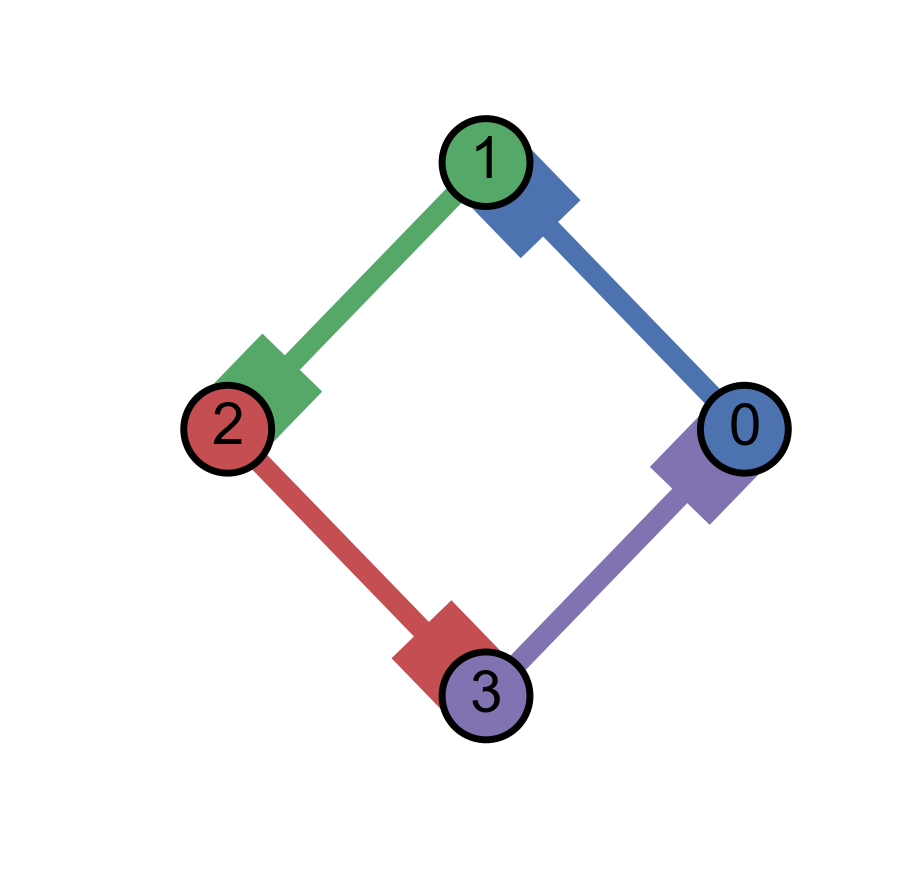
\includegraphics[width=0.4\linewidth,keepaspectratio,trim={0 3cm 0 2cm},clip]{./simulation/cycle/cycle_4.png}\label{fig:cycle_4}}\qquad
			\subfloat[][]{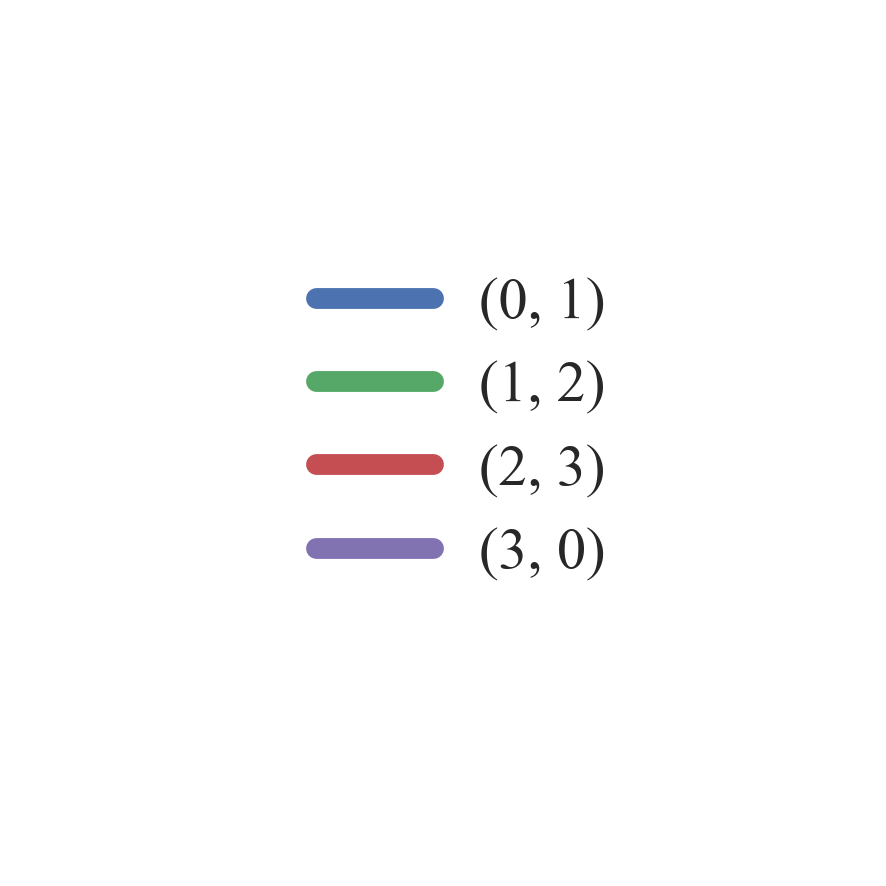
\includegraphics[width=0.4\linewidth,keepaspectratio,trim={0 3cm 0 2cm},clip]{./simulation/cycle/cycle_4_legend.png}\label{fig:cycle_4_legend}}
			\newline
			\subfloat[][]{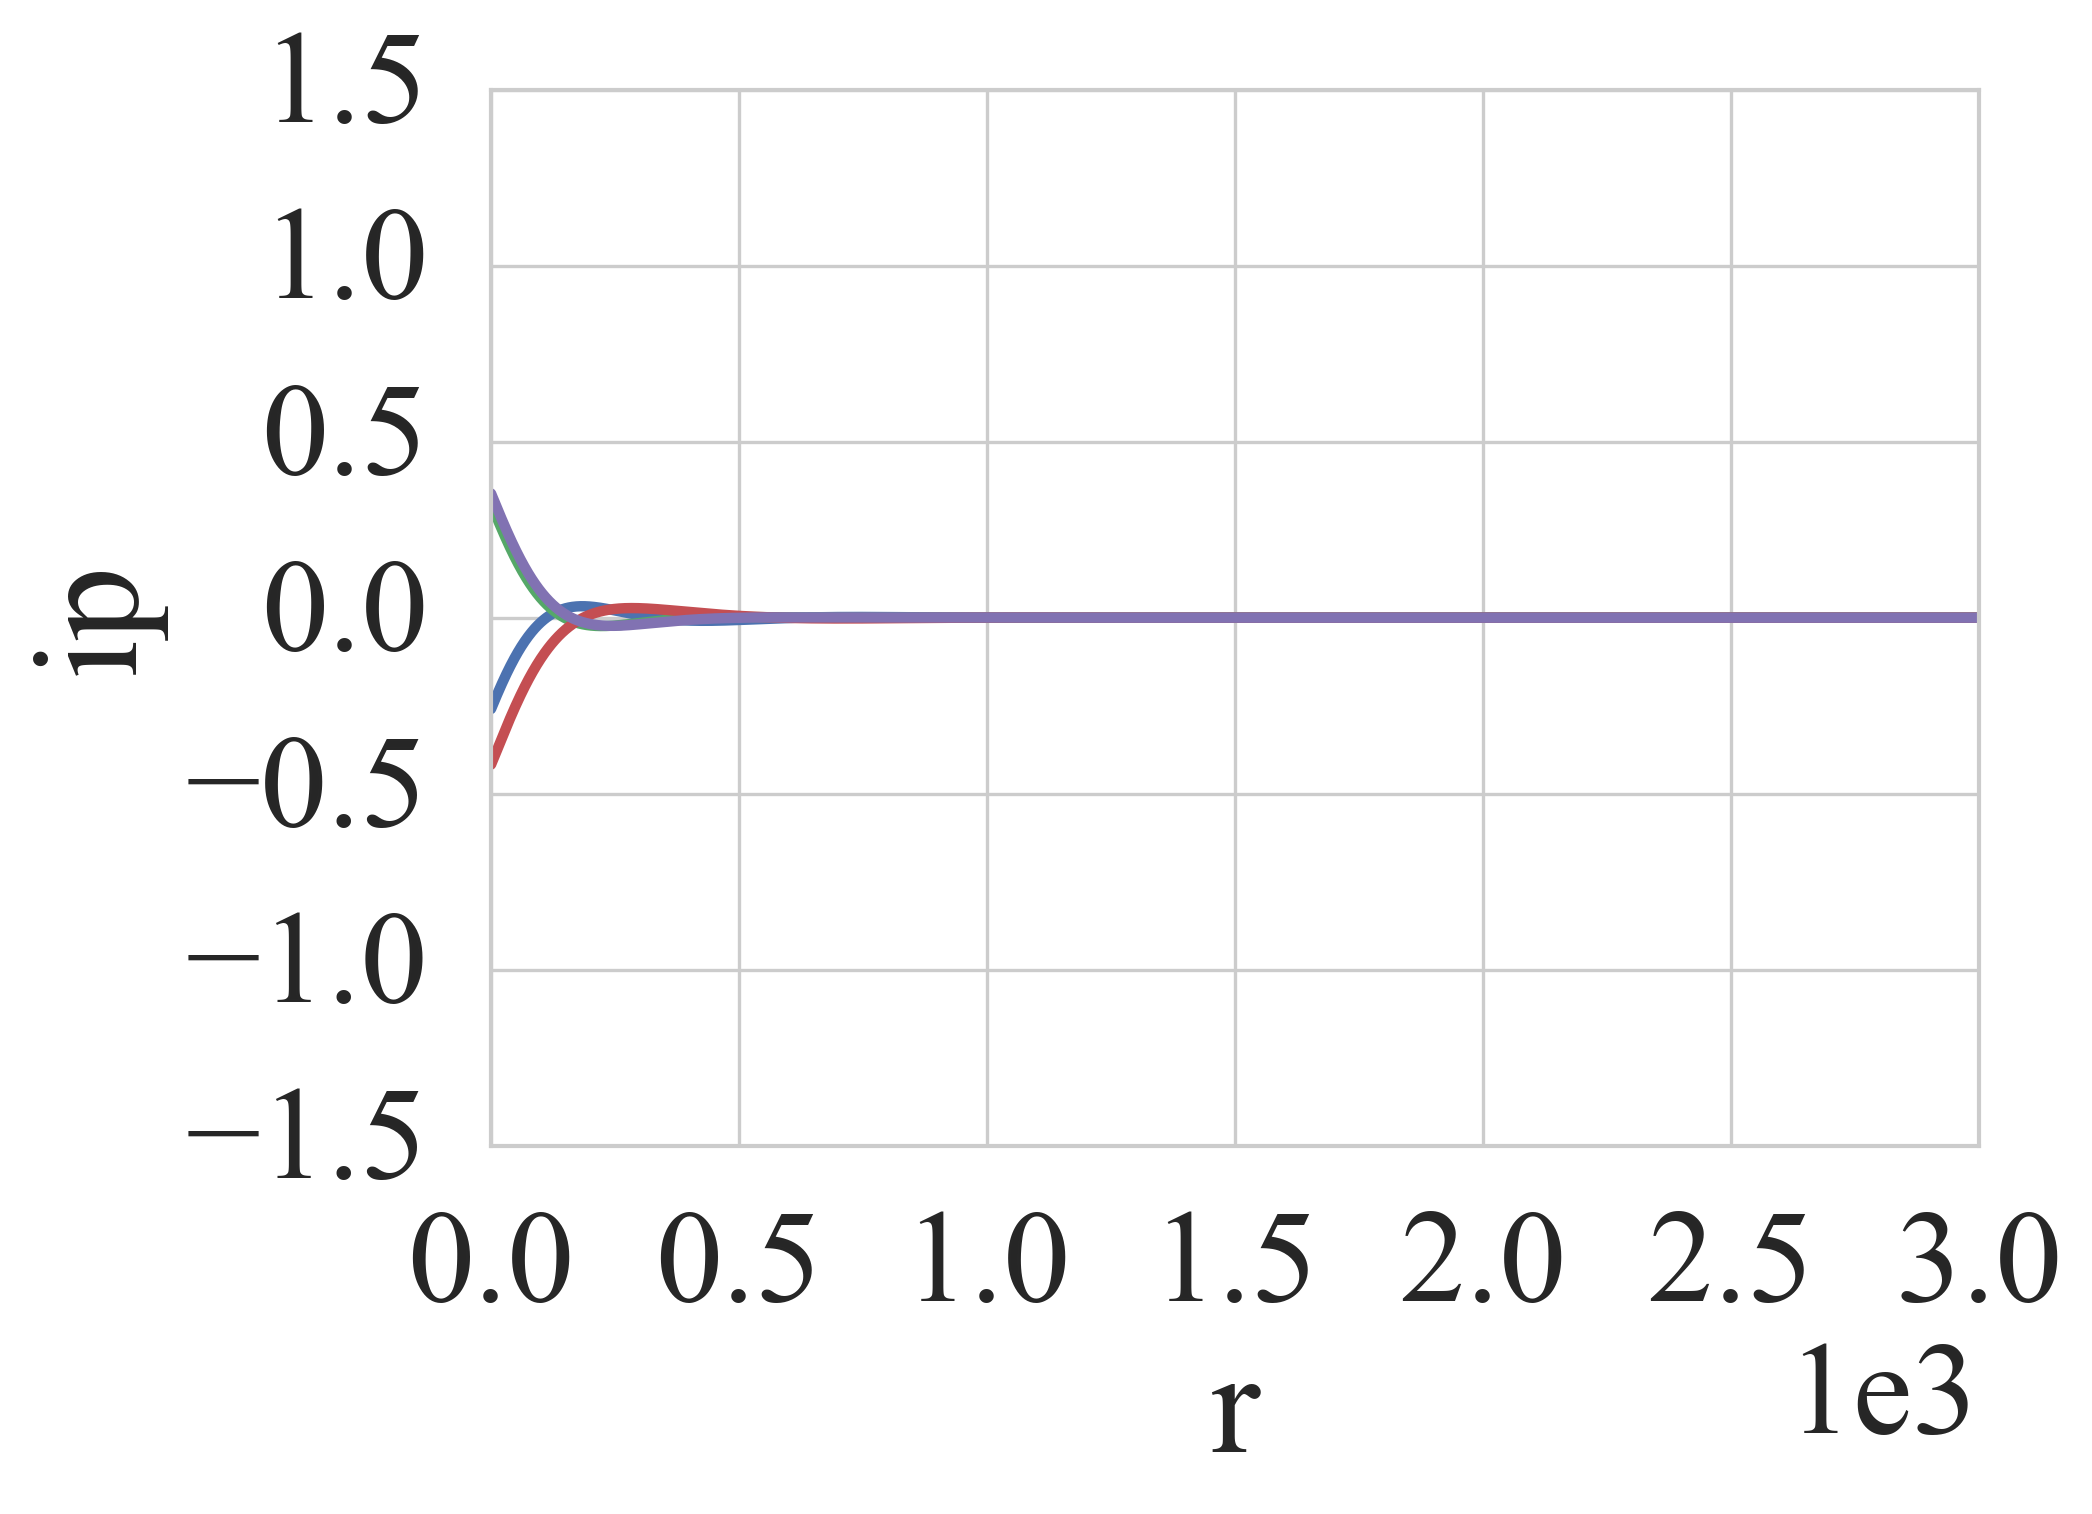
\includegraphics[width=0.4\linewidth,keepaspectratio]{./simulation/cycle/cycle_4_ip_zero.png}\label{fig:cycle_4_ip_zero}}\qquad
			\subfloat[][]{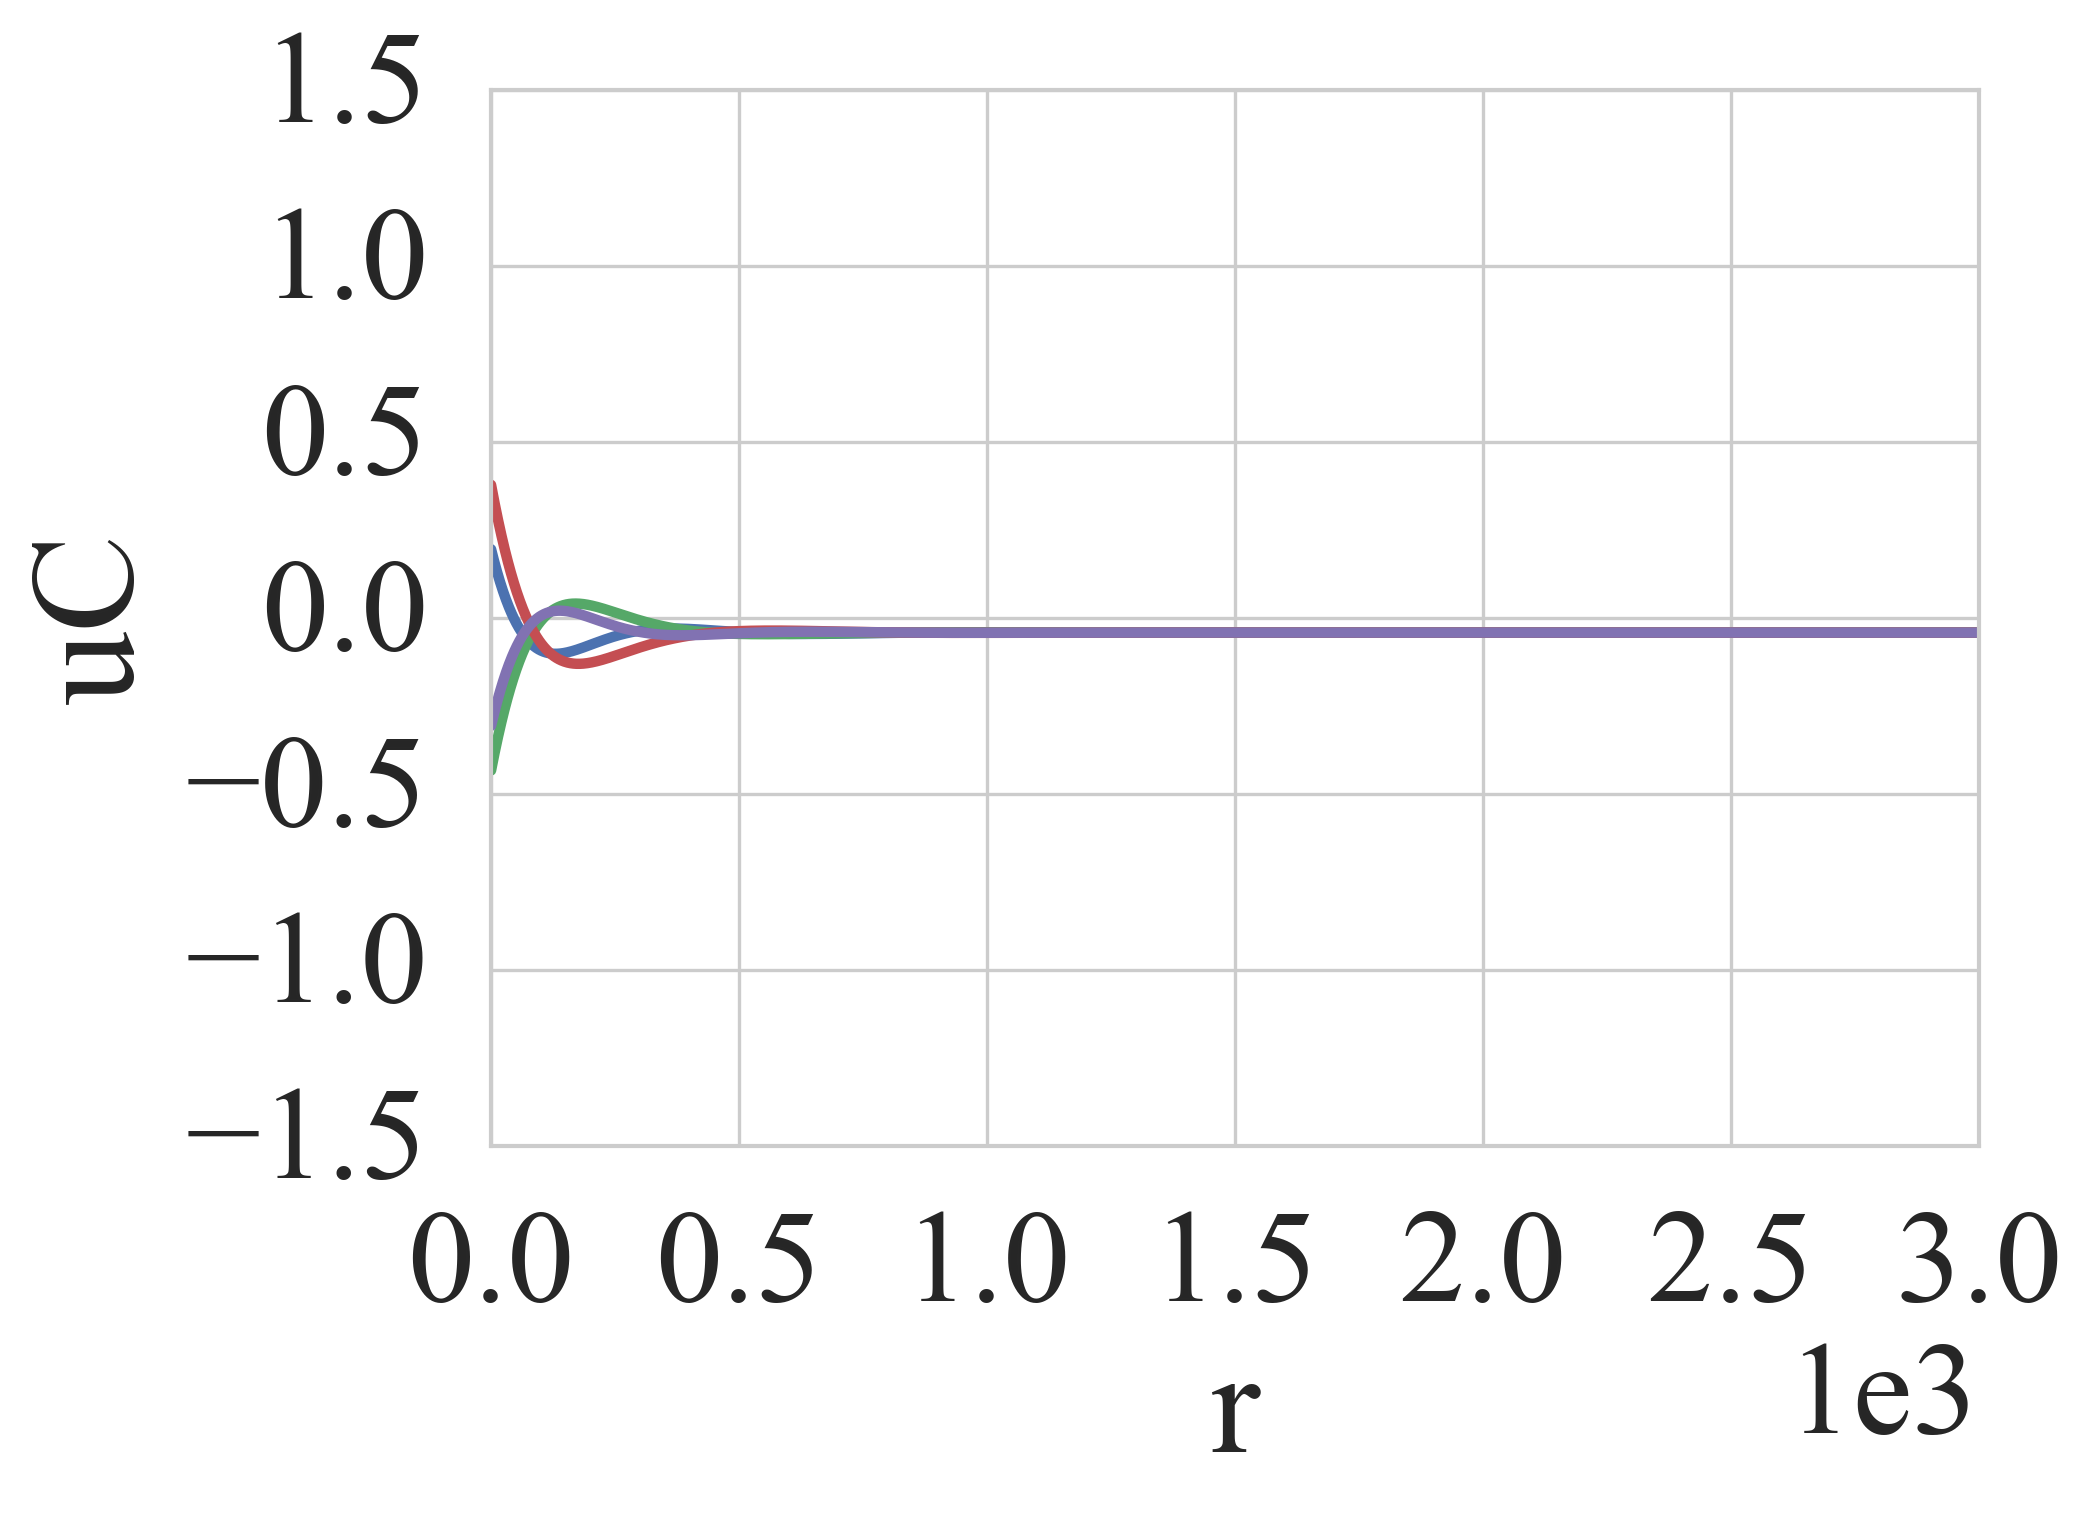
\includegraphics[width=0.4\linewidth,keepaspectratio]{./simulation/cycle/cycle_4_uC_zero.png}\label{fig:cycle_4_uC_zero}}
			\newline
			\subfloat[][]{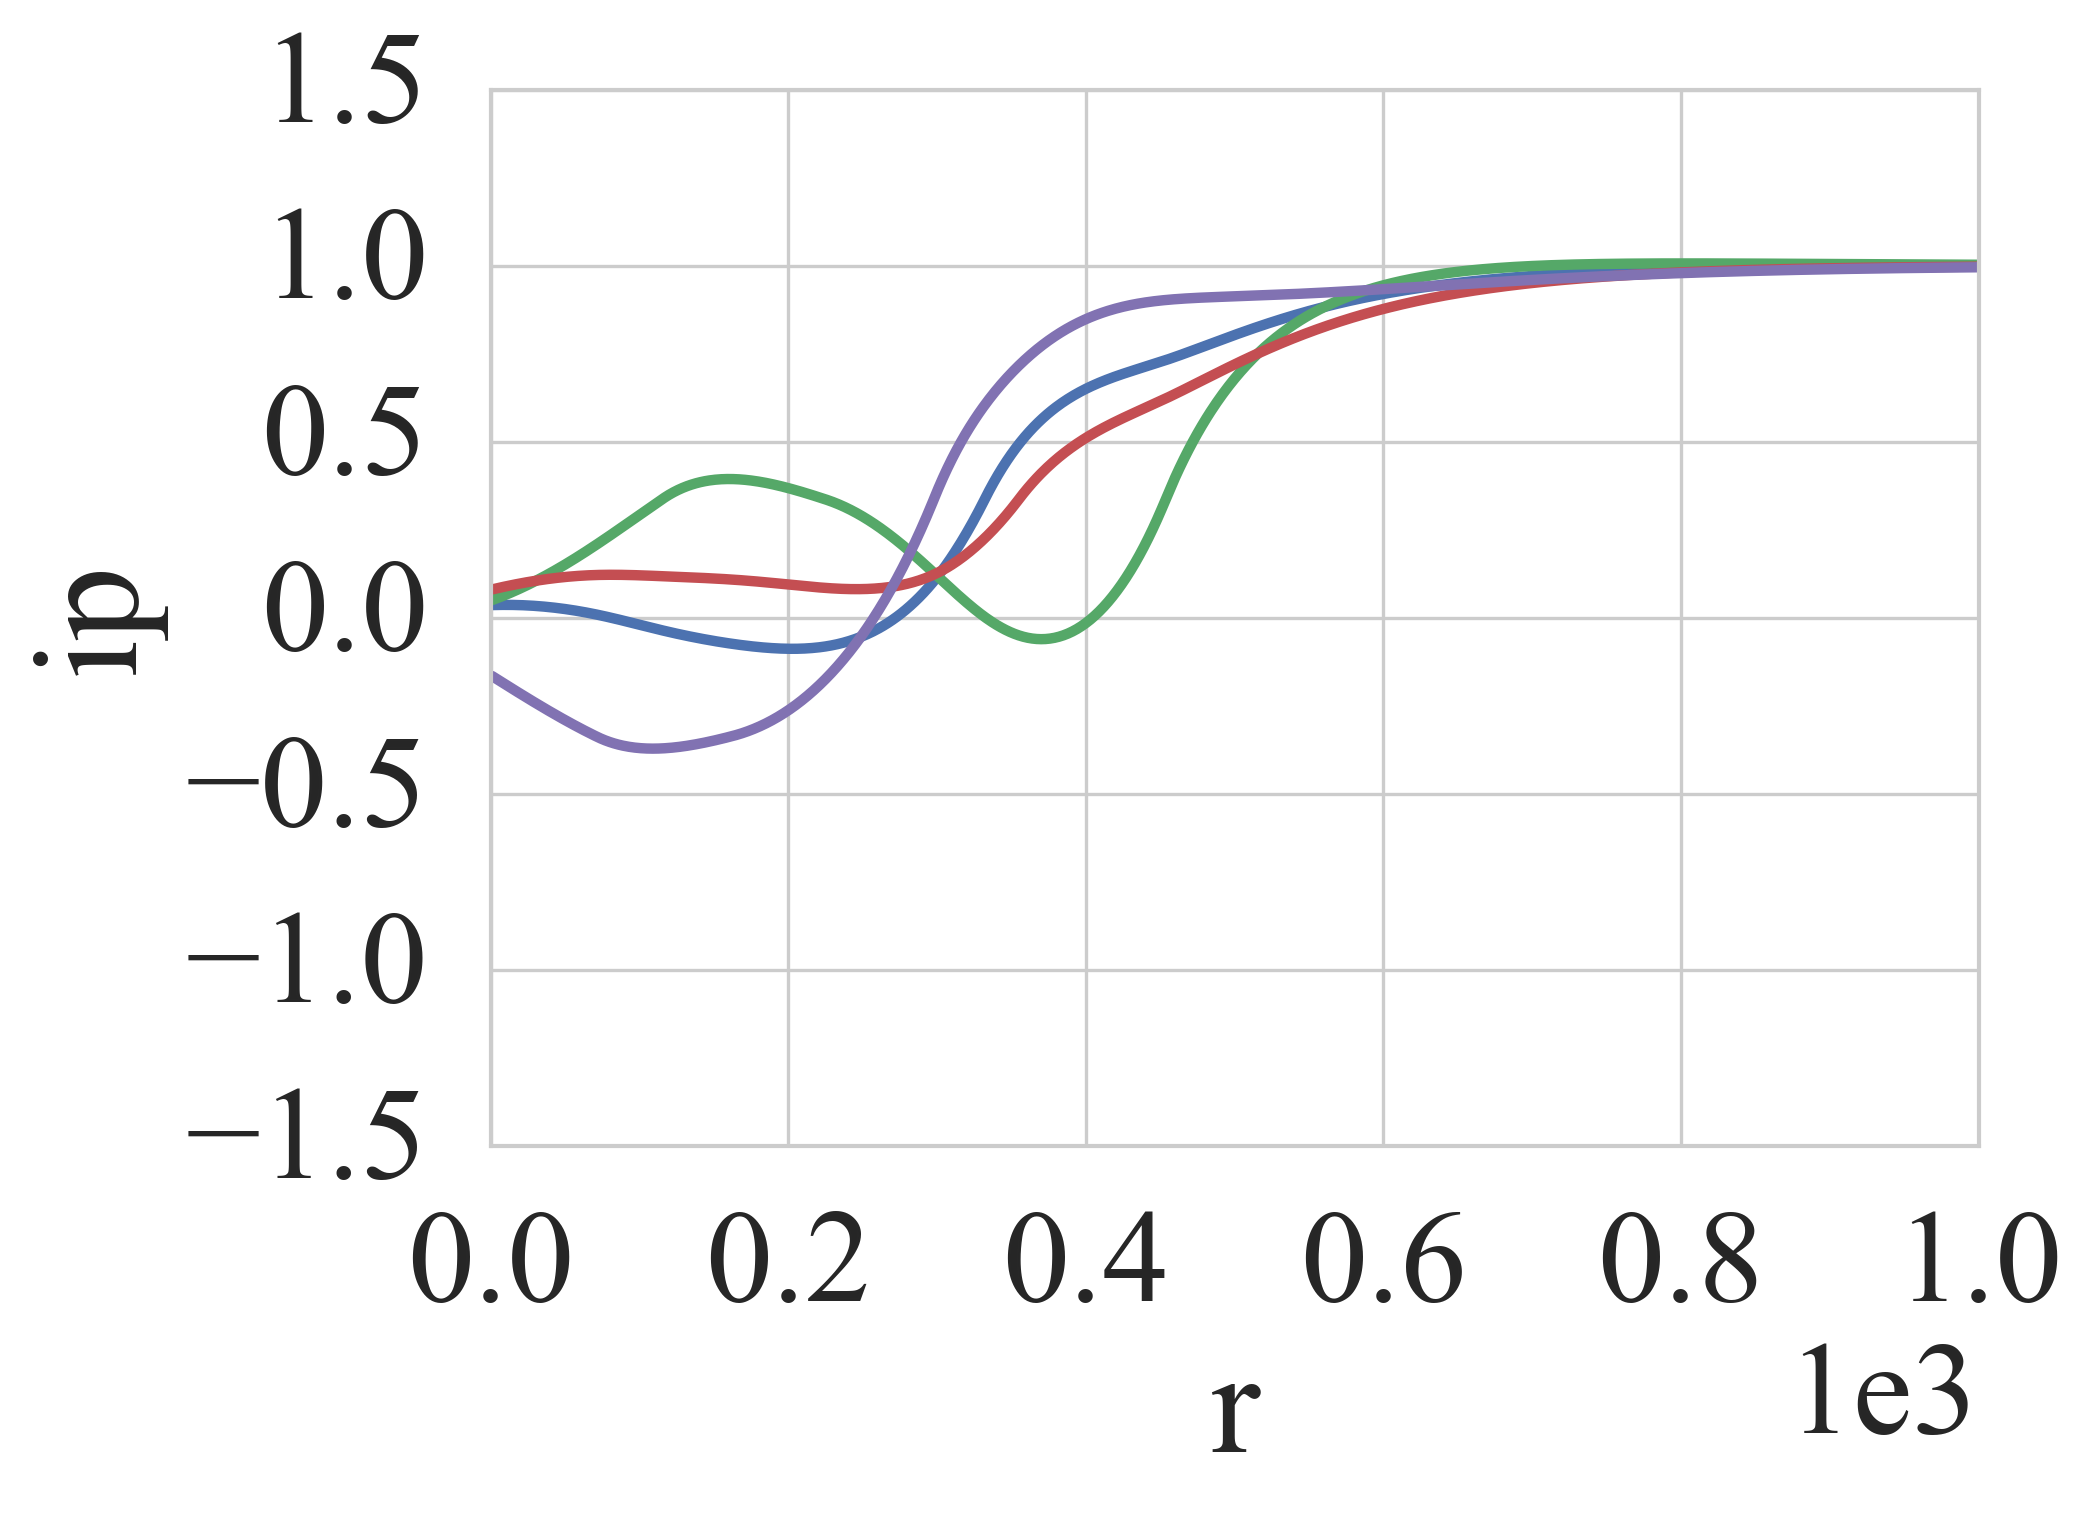
\includegraphics[width=0.4\linewidth,keepaspectratio]{./simulation/cycle/cycle_4_ip_positive.png}\label{fig:cycle_4_ip_positive}}\qquad
			\subfloat[][]{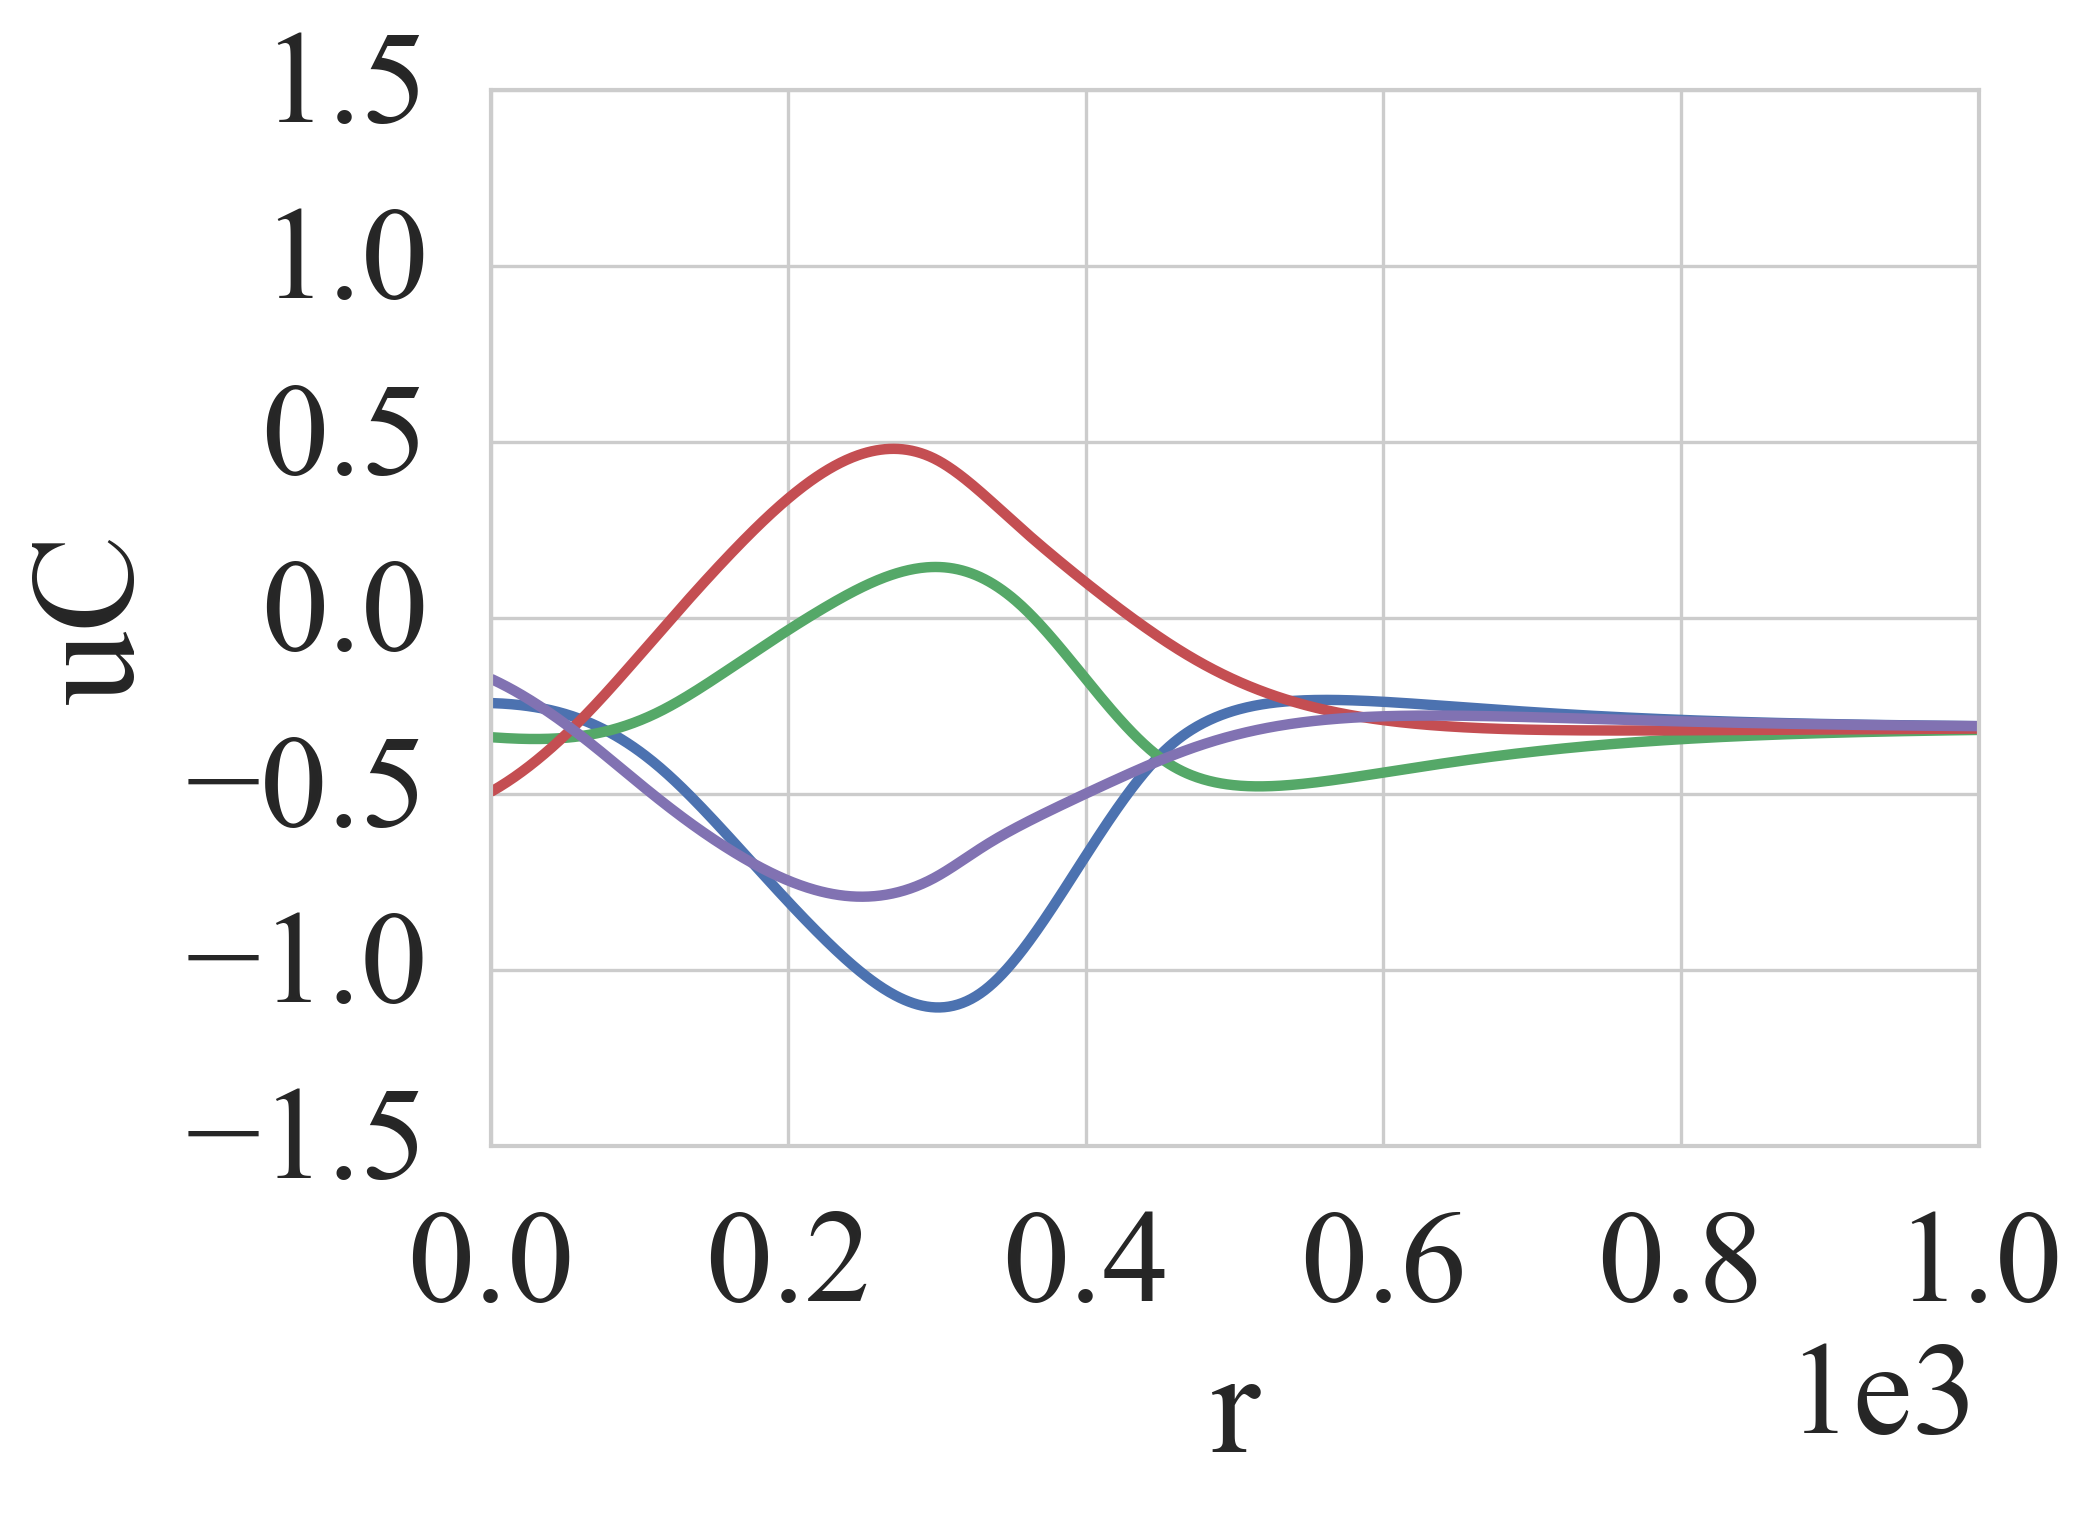
\includegraphics[width=0.4\linewidth,keepaspectratio]{./simulation/cycle/cycle_4_uC_positive.png}\label{fig:cycle_4_uC_positive}}
			\newline
			\subfloat[][]{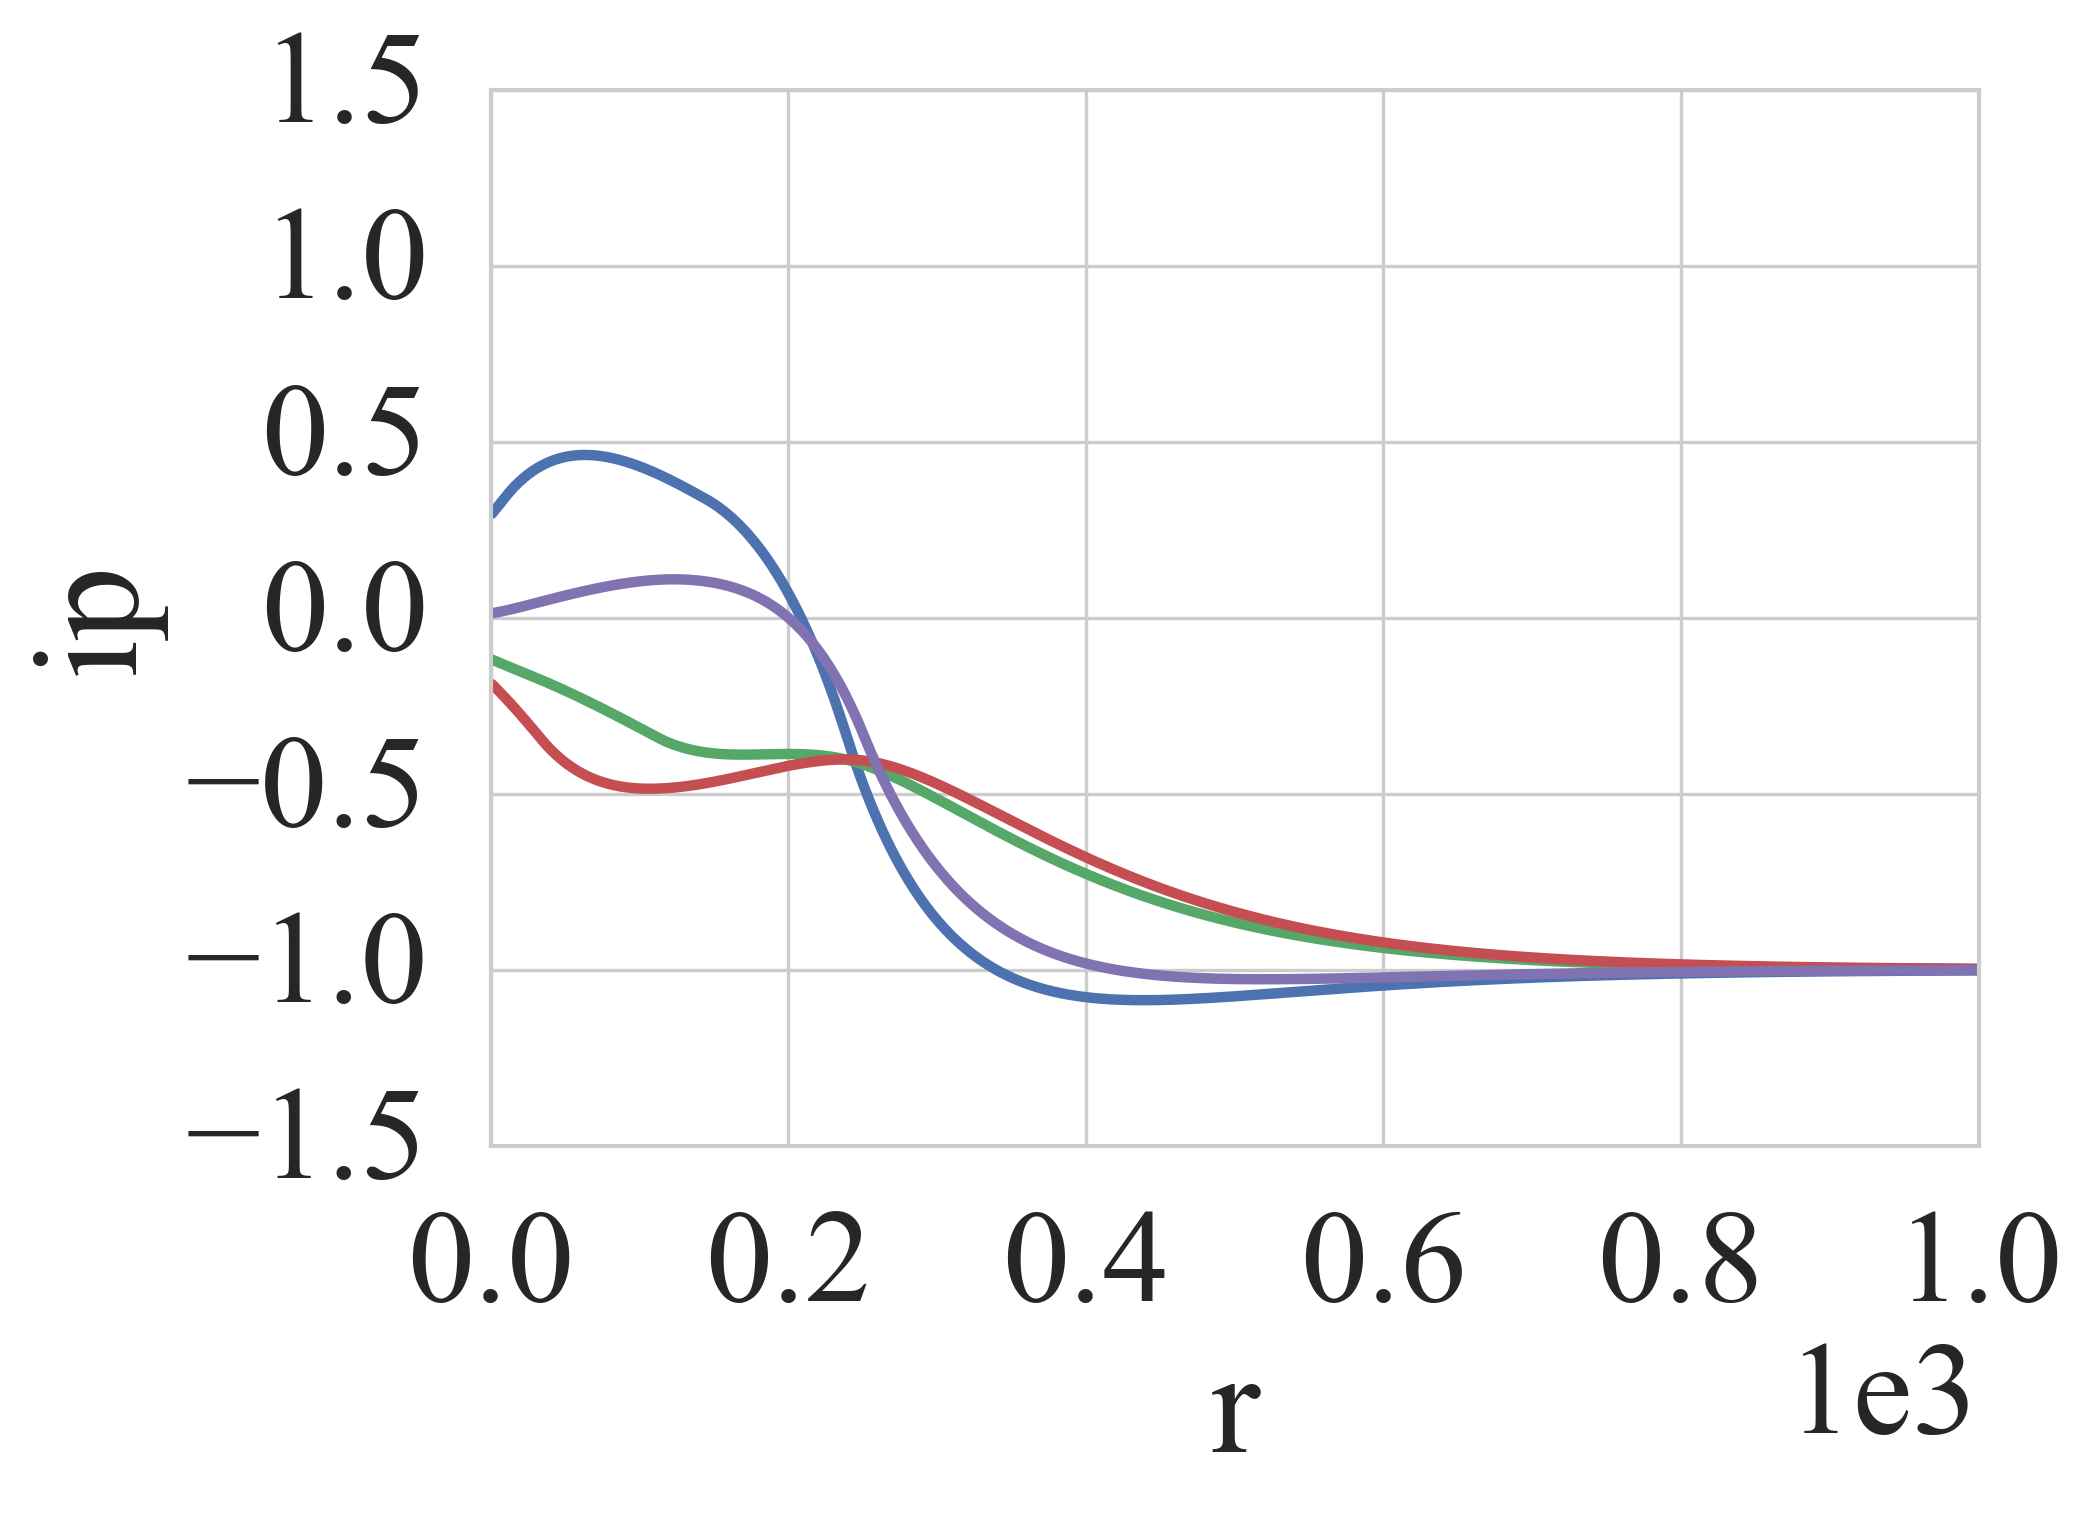
\includegraphics[width=0.4\linewidth,keepaspectratio]{./simulation/cycle/cycle_4_ip_negative.png}\label{fig:cycle_4_ip_negative}}\qquad
			\subfloat[][]{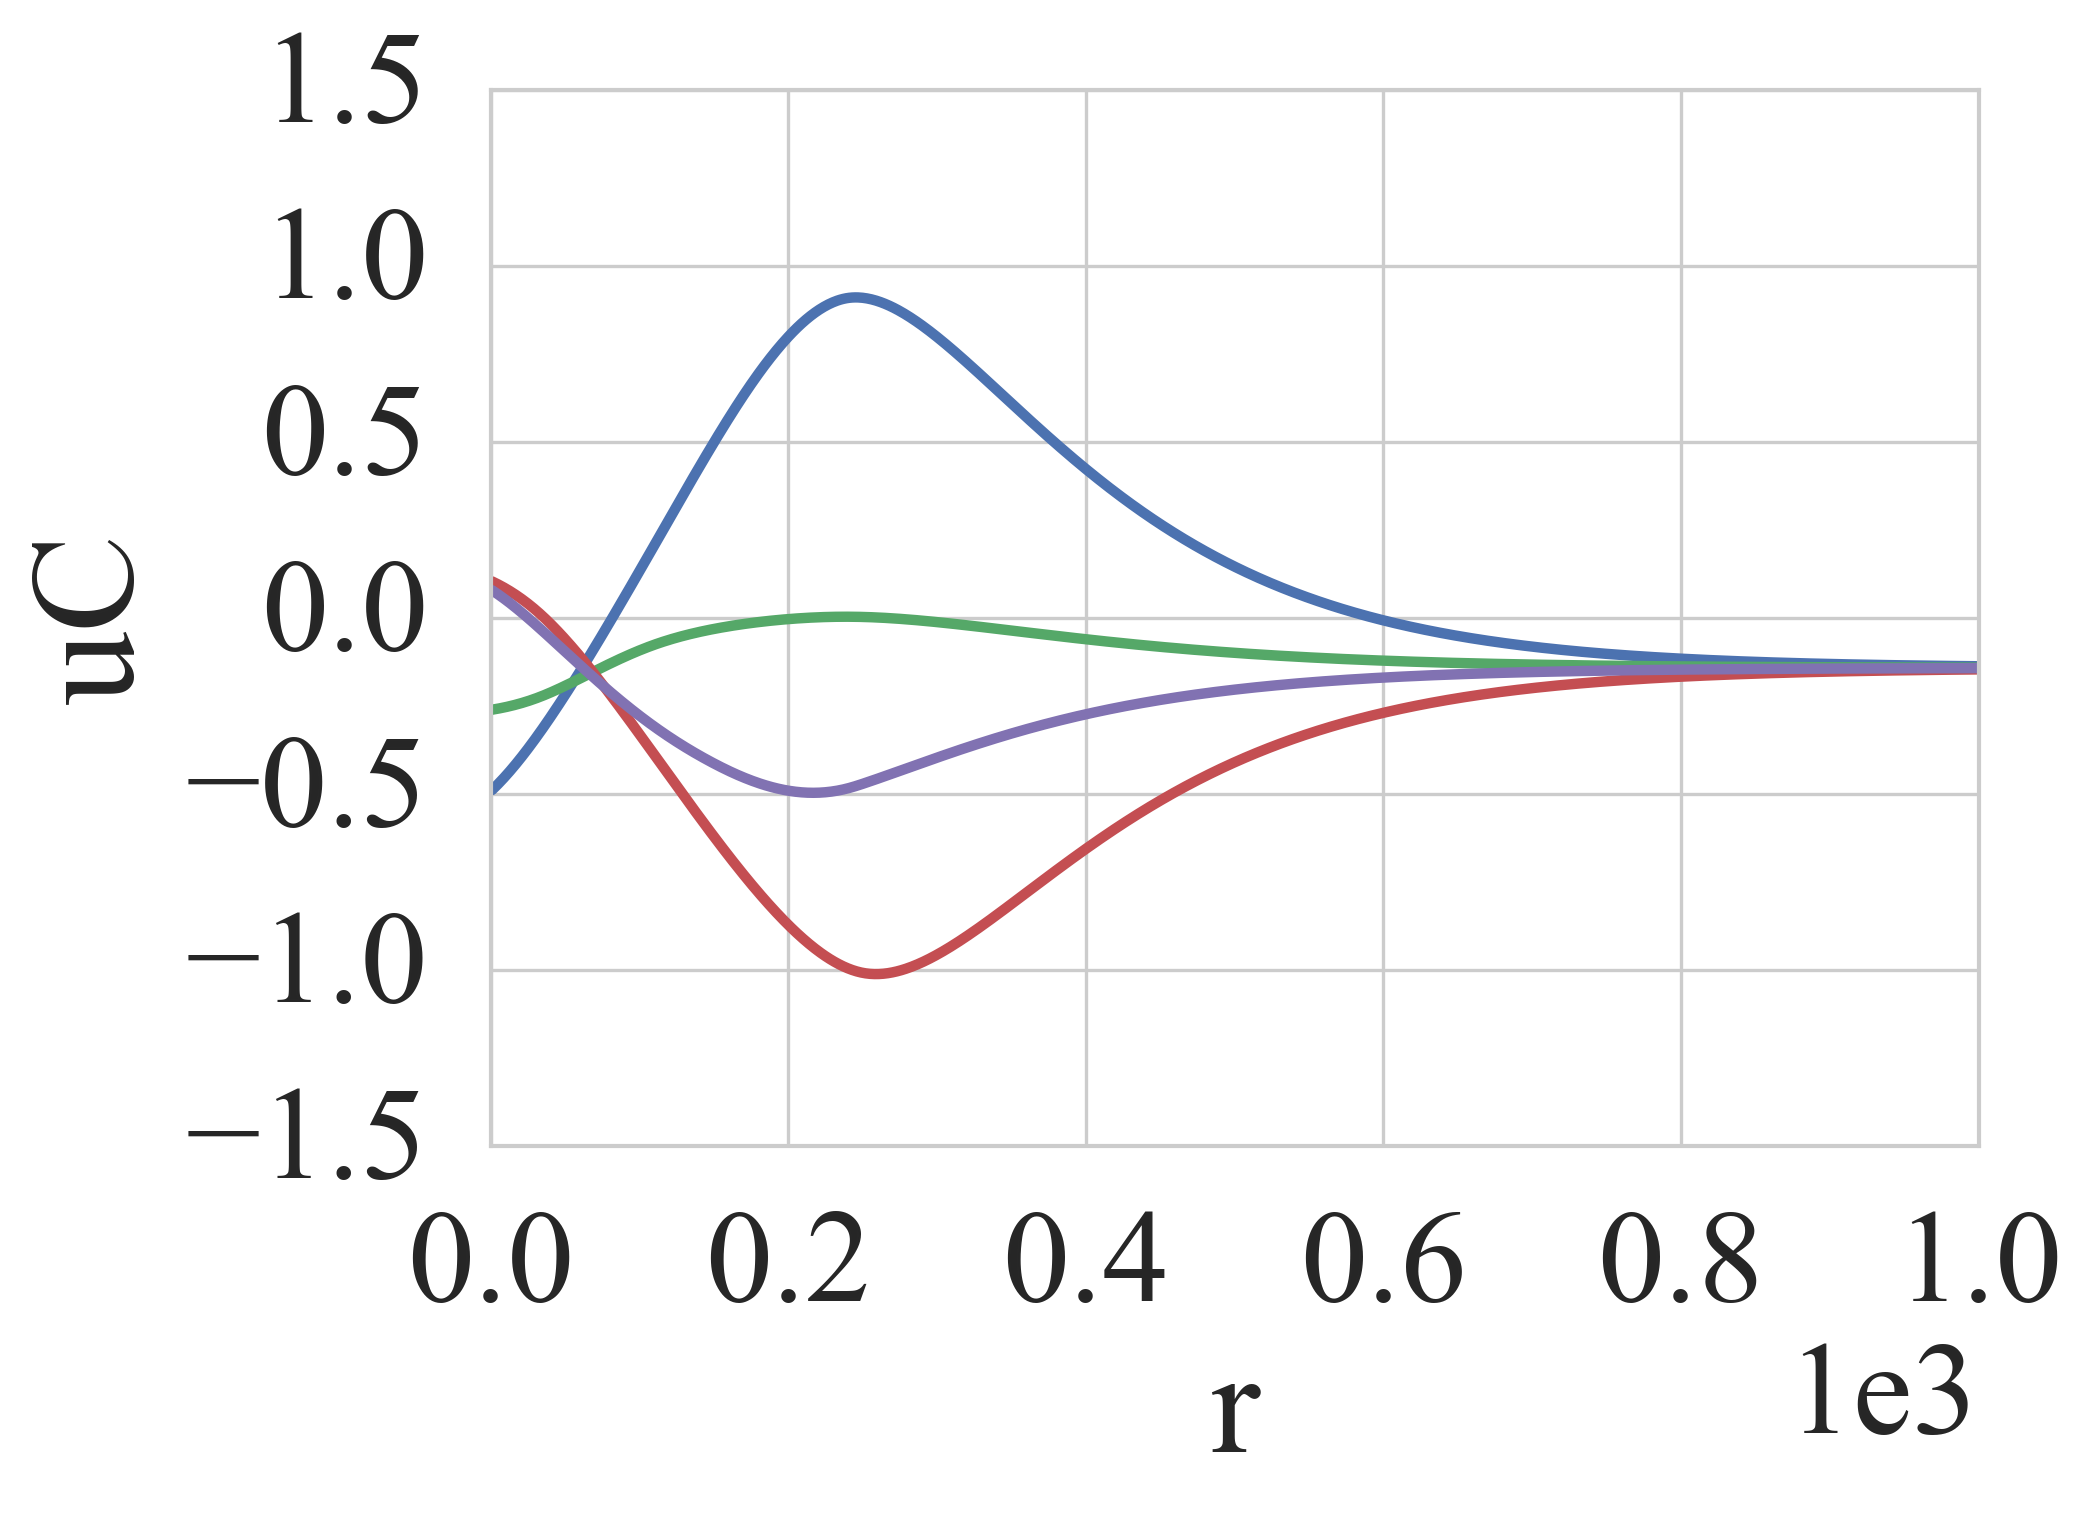
\includegraphics[width=0.4\linewidth,keepaspectratio]{./simulation/cycle/cycle_4_uC_negative.png}\label{fig:cycle_4_uC_negative}}
			
			\caption[Cycle simulations]{Simulation experiments for a cycle of $4$ \Pes.}
			\label{fig:cycle}
		\end{figure}

	\subsection{Diamond of \emph{Physarum} Elements}

		The graph we investigate is the so-called diamond graph depicted in \Fref{fig:diamond_graph}. This topology is also widely known under the name of Wheatstone graph or Wheatstone bridge. It consists of a $4$-cycle with an additional ``bridge'' edge $(2,0)$ added. Again \Fref{fig:diamond_graph_legend} defines a color coding which serves as a legend for the remaining plots of \Fref{fig:diamond}. We show the results of three distinct runs of the simulation.

		Similar to the $4$-cycle explored previously, we investigate several scenarios. In all of them the capacitor voltages quickly converge $u_{C,e}(t)$, see \Fref{fig:diamond_ip_asymmetric_positive}, \Fref{fig:diamond_ip_symmetric_negative} and \Fref{fig:diamond_ip_asymmetric_positive}. However, due to the additional edge introduced to the \Pn, edges do not converge to the same values anymore but split up in three distinct groups. The first group is formed by edges $(0,1)$ and $(1,2)$. The second group are edges $(2,3)$ and $(3,0)$. And the last group is the bridge edge $(2,0)$. Note that all in all shown scenarios the voltages show that the first two groups are symmetric around the value the center edge converges to. Although the capacitor voltages show identical behavior, very different currents can be accommodated.

		\Fref{fig:diamond_ip_symmetric_positive} shows a scenario, where $1.5$ units of current flow through the center edge to split evenly at node $0$. The split flow then circles back to node $2$ showing appropriate signs and values. \Fref{fig:diamond_ip_symmetric_negative} shows the same situation but with the flow on the center edge reversed. Naturally, there is no reason to assume that flow must split up symmetrically. \Fref{fig:diamond_ip_asymmetric_positive} shows one of many possible unbalanced scenarios. As in the case of the $4$-cycle, we do not know the details of the splitting process nor its dependence on initial conditions at this point.

		\begin{figure}
			\centering
			\subfloat[][]{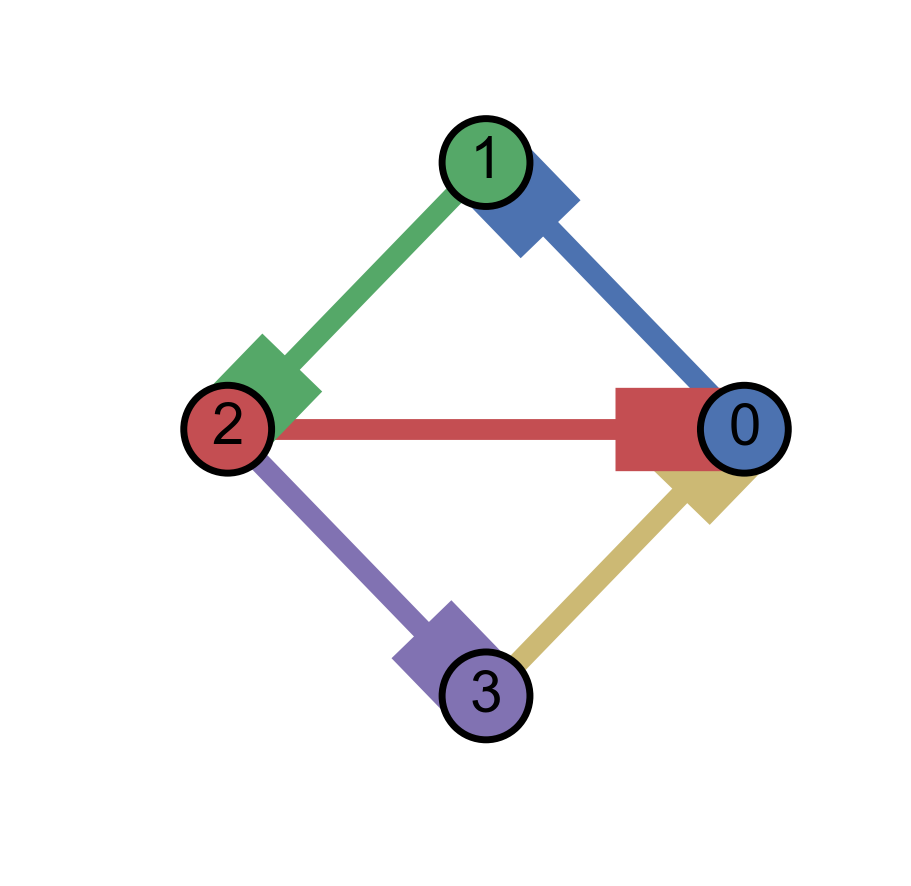
\includegraphics[width=0.4\linewidth,keepaspectratio,trim={0 3cm 0 2cm},clip]{./simulation/diamond/diamond.png}\label{fig:diamond_graph}}\qquad
			\subfloat[][]{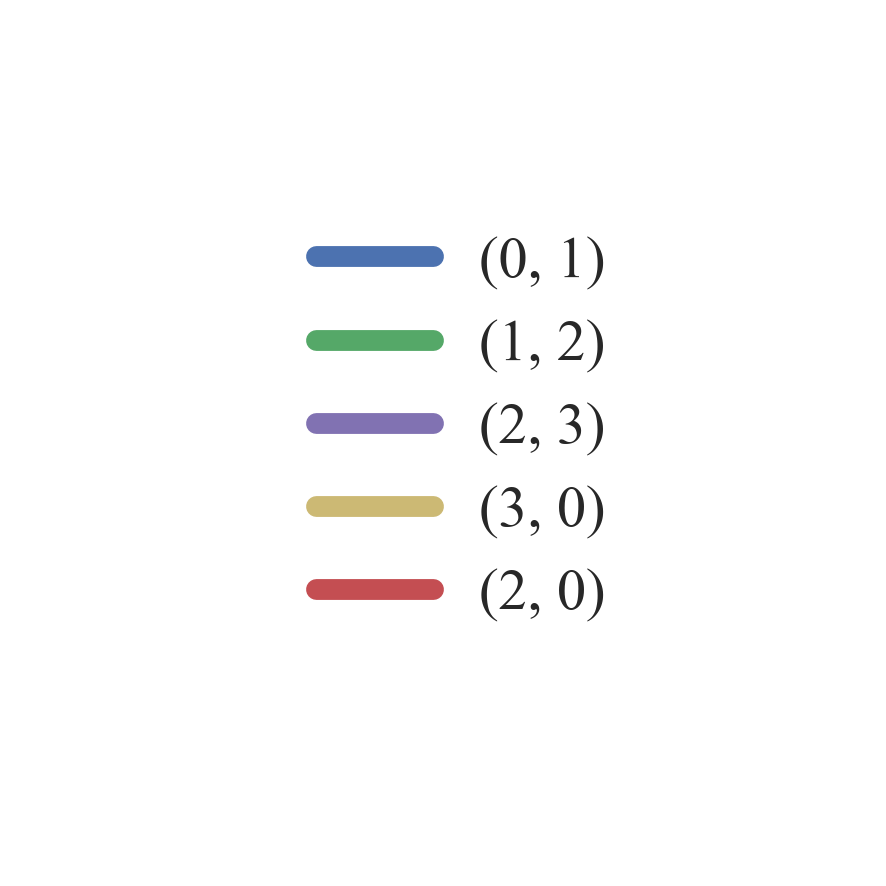
\includegraphics[width=0.4\linewidth,keepaspectratio,trim={0 3cm 0 2cm},clip]{./simulation/diamond/diamond_legend.png}\label{fig:diamond_graph_legend}}
			\newline
			\subfloat[][]{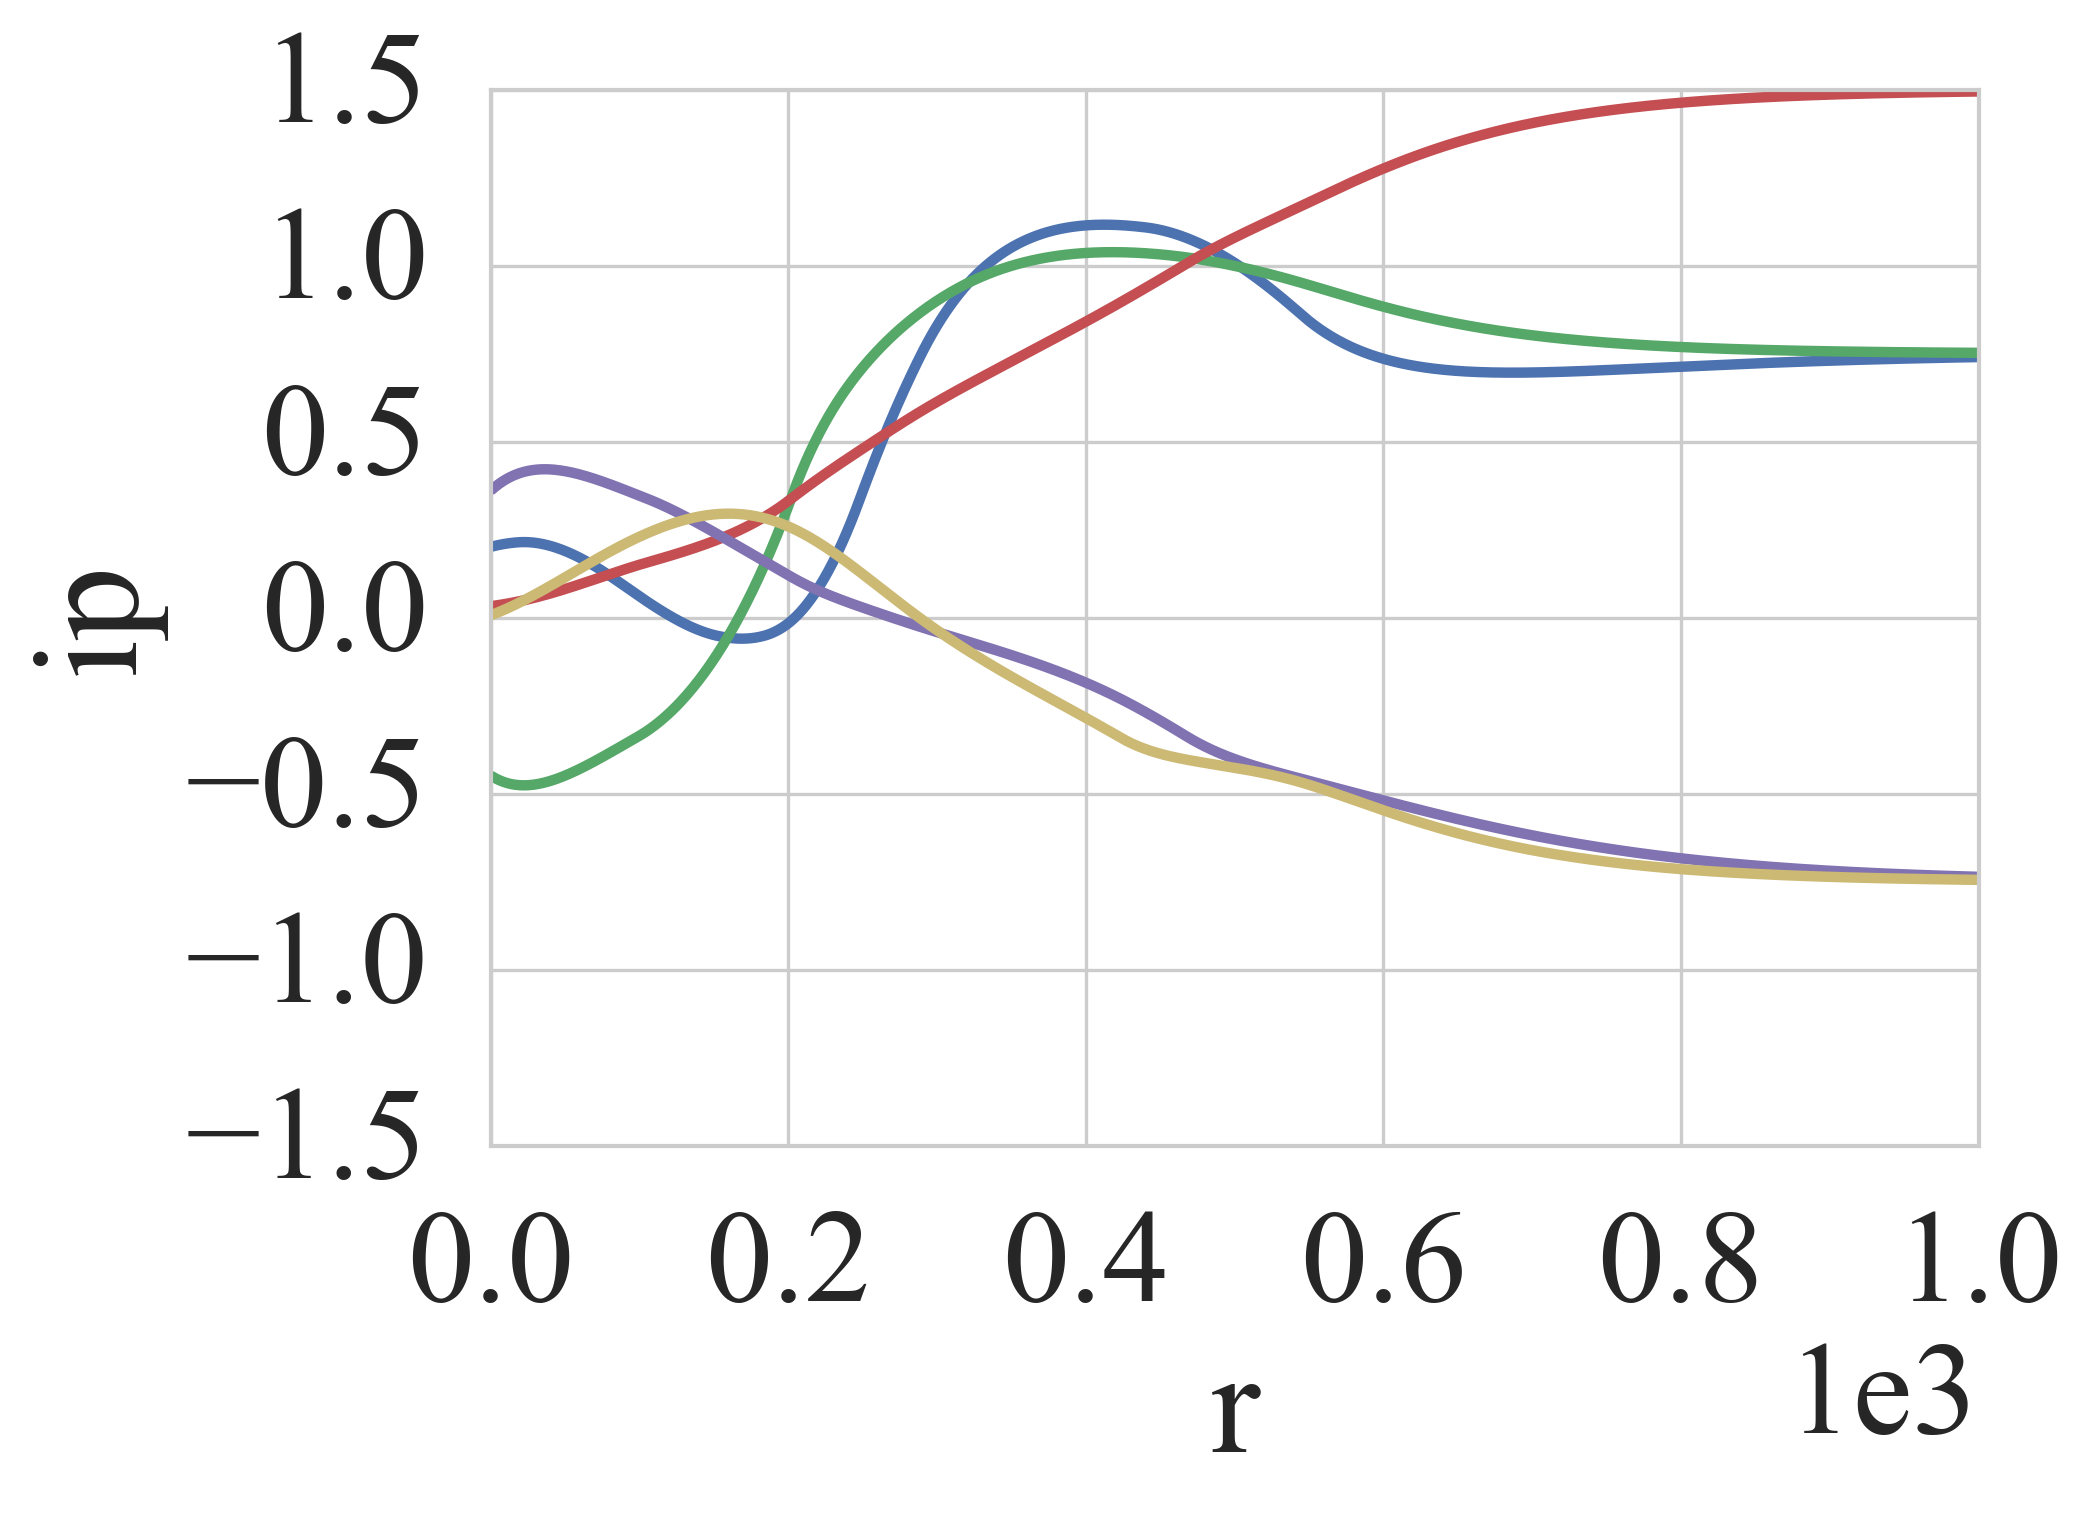
\includegraphics[width=0.4\linewidth,keepaspectratio]{./simulation/diamond/diamond_ip_symmetric_positive.png}\label{fig:diamond_ip_symmetric_positive}}\qquad
			\subfloat[][]{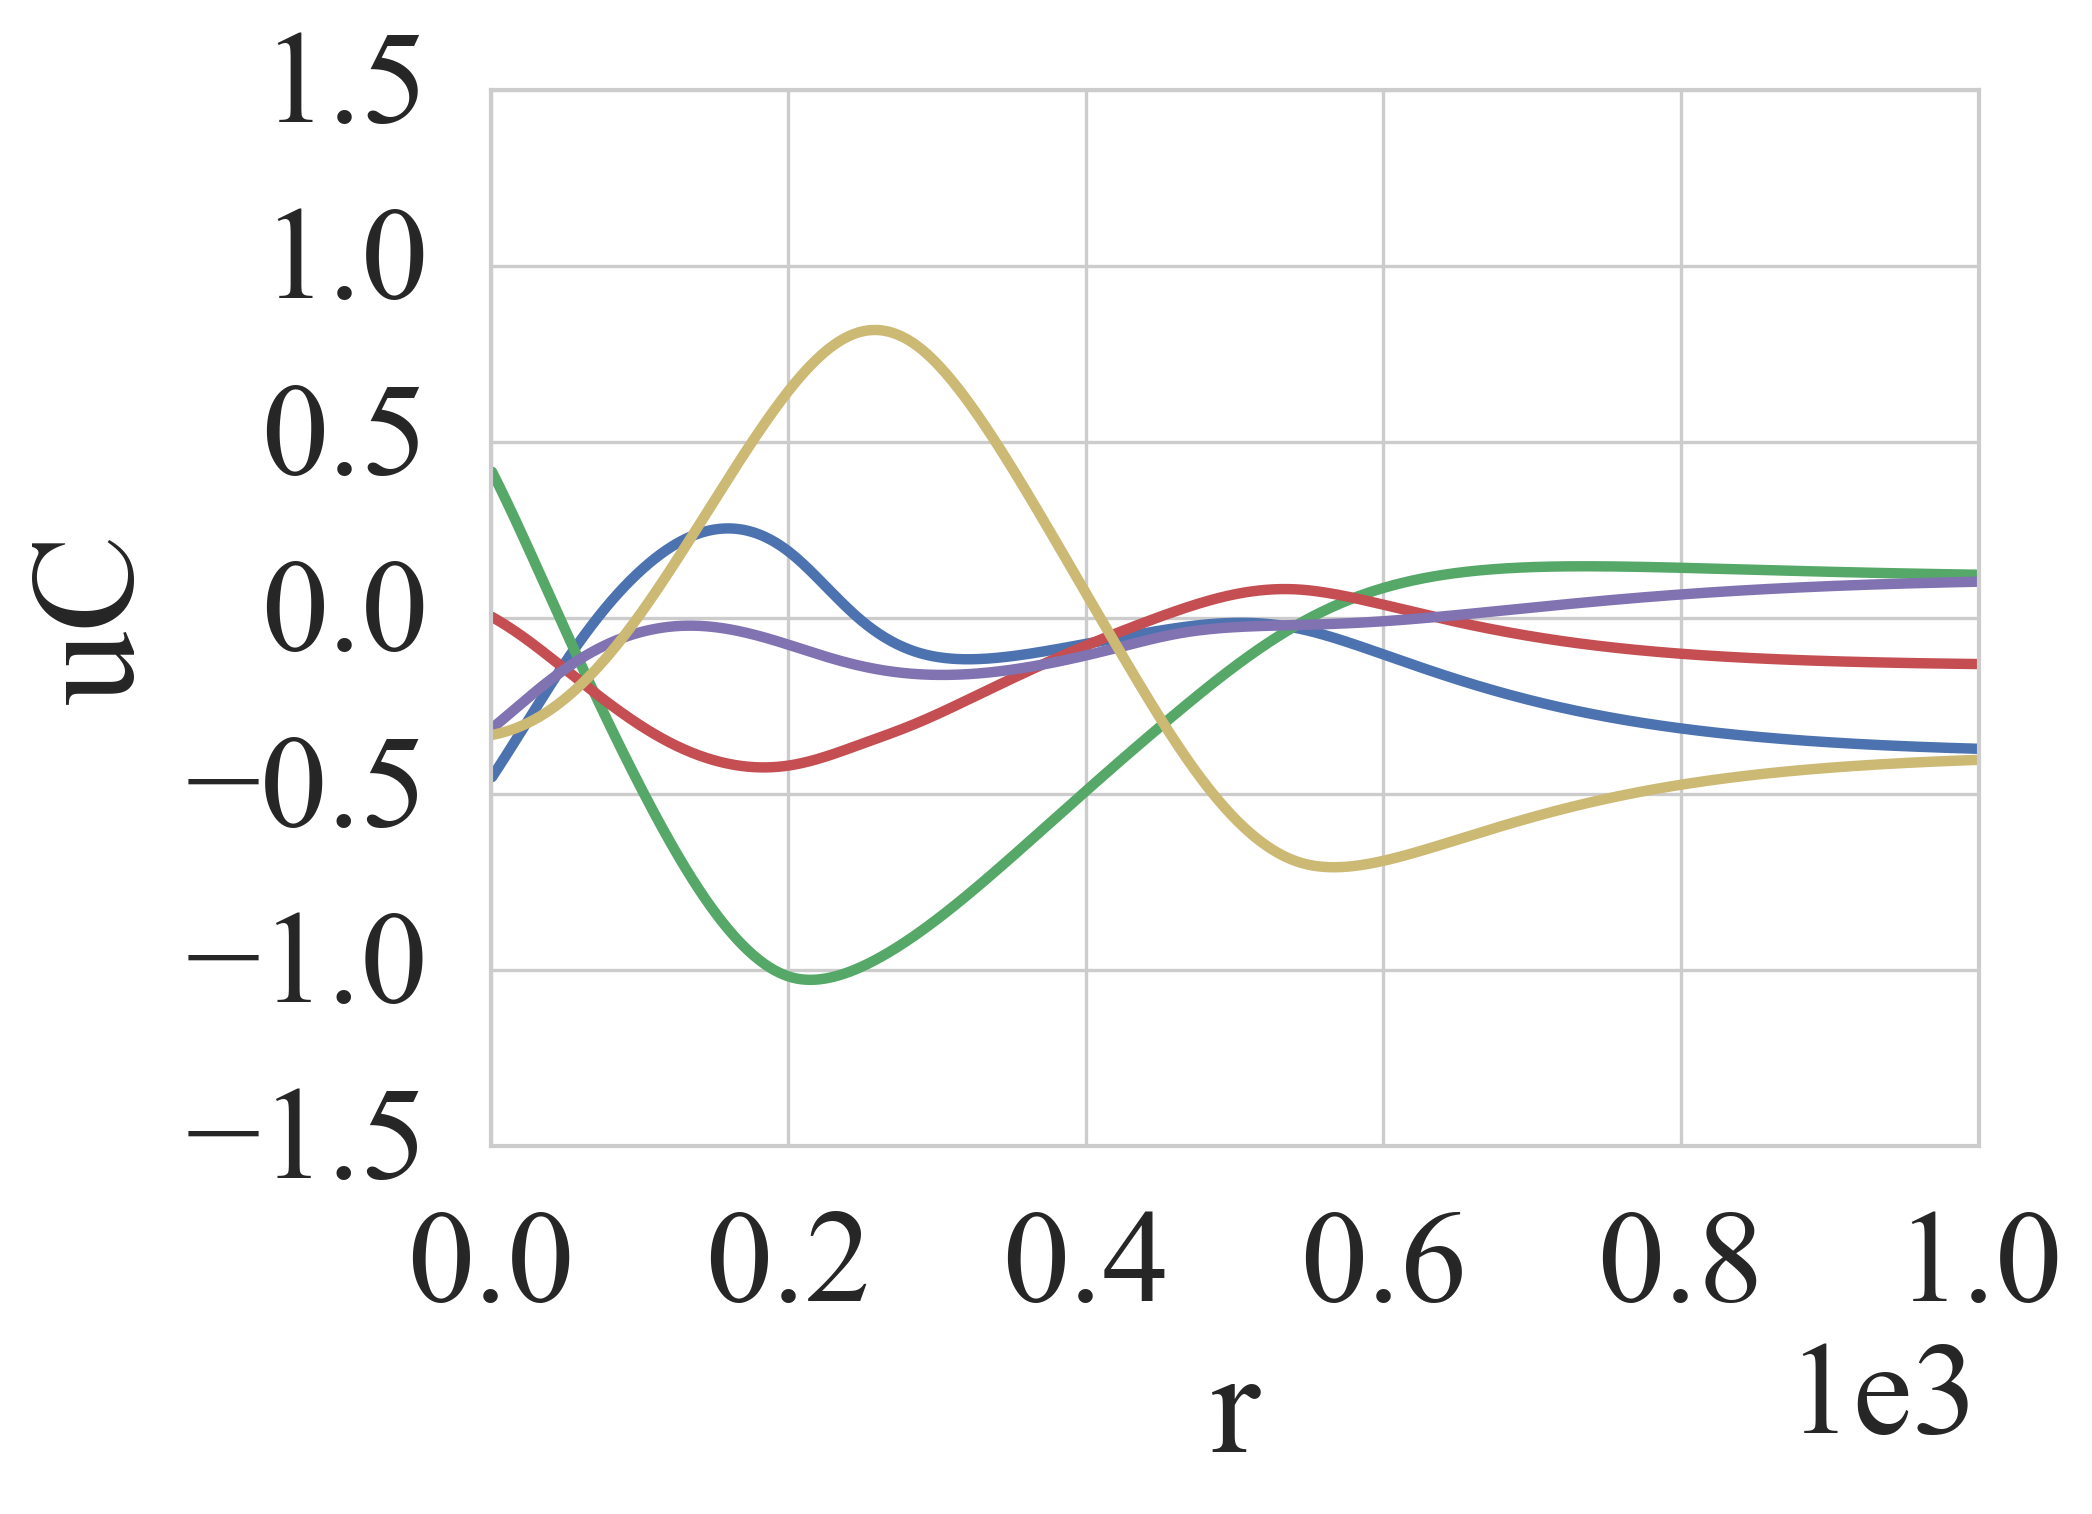
\includegraphics[width=0.4\linewidth,keepaspectratio]{./simulation/diamond/diamond_uC_symmetric_positive.png}\label{fig:diamond_uC_symmetric_positive}}
			\newline
			\subfloat[][]{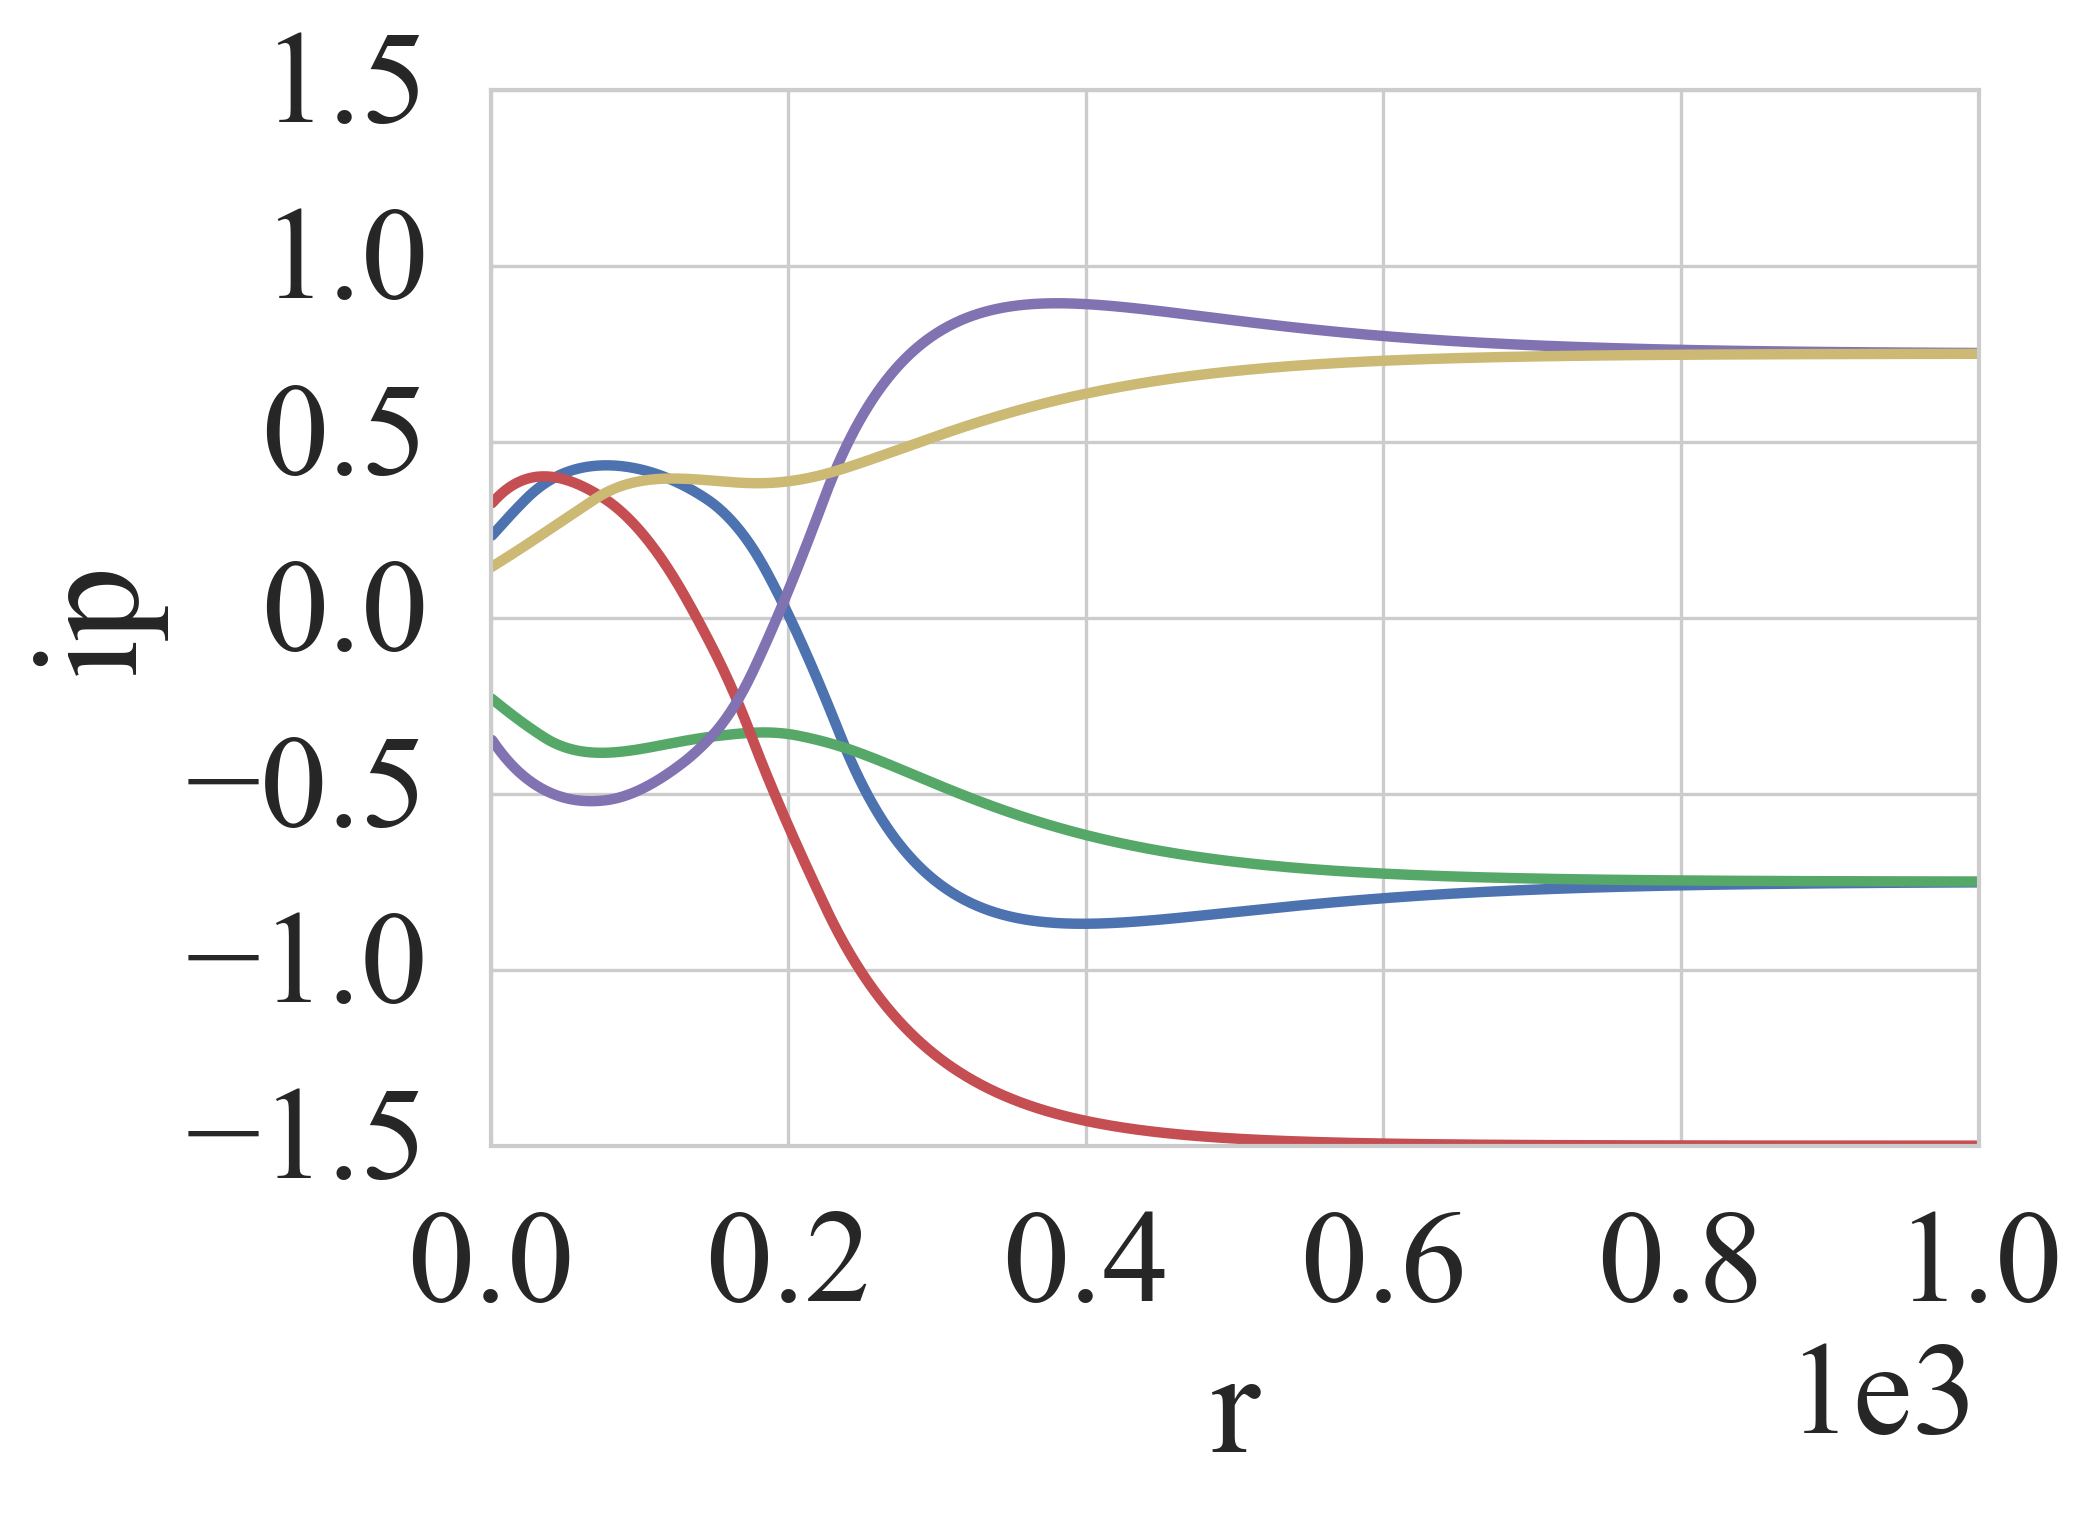
\includegraphics[width=0.4\linewidth,keepaspectratio]{./simulation/diamond/diamond_ip_symmetric_negative.png}\label{fig:diamond_ip_symmetric_negative}}\qquad
			\subfloat[][]{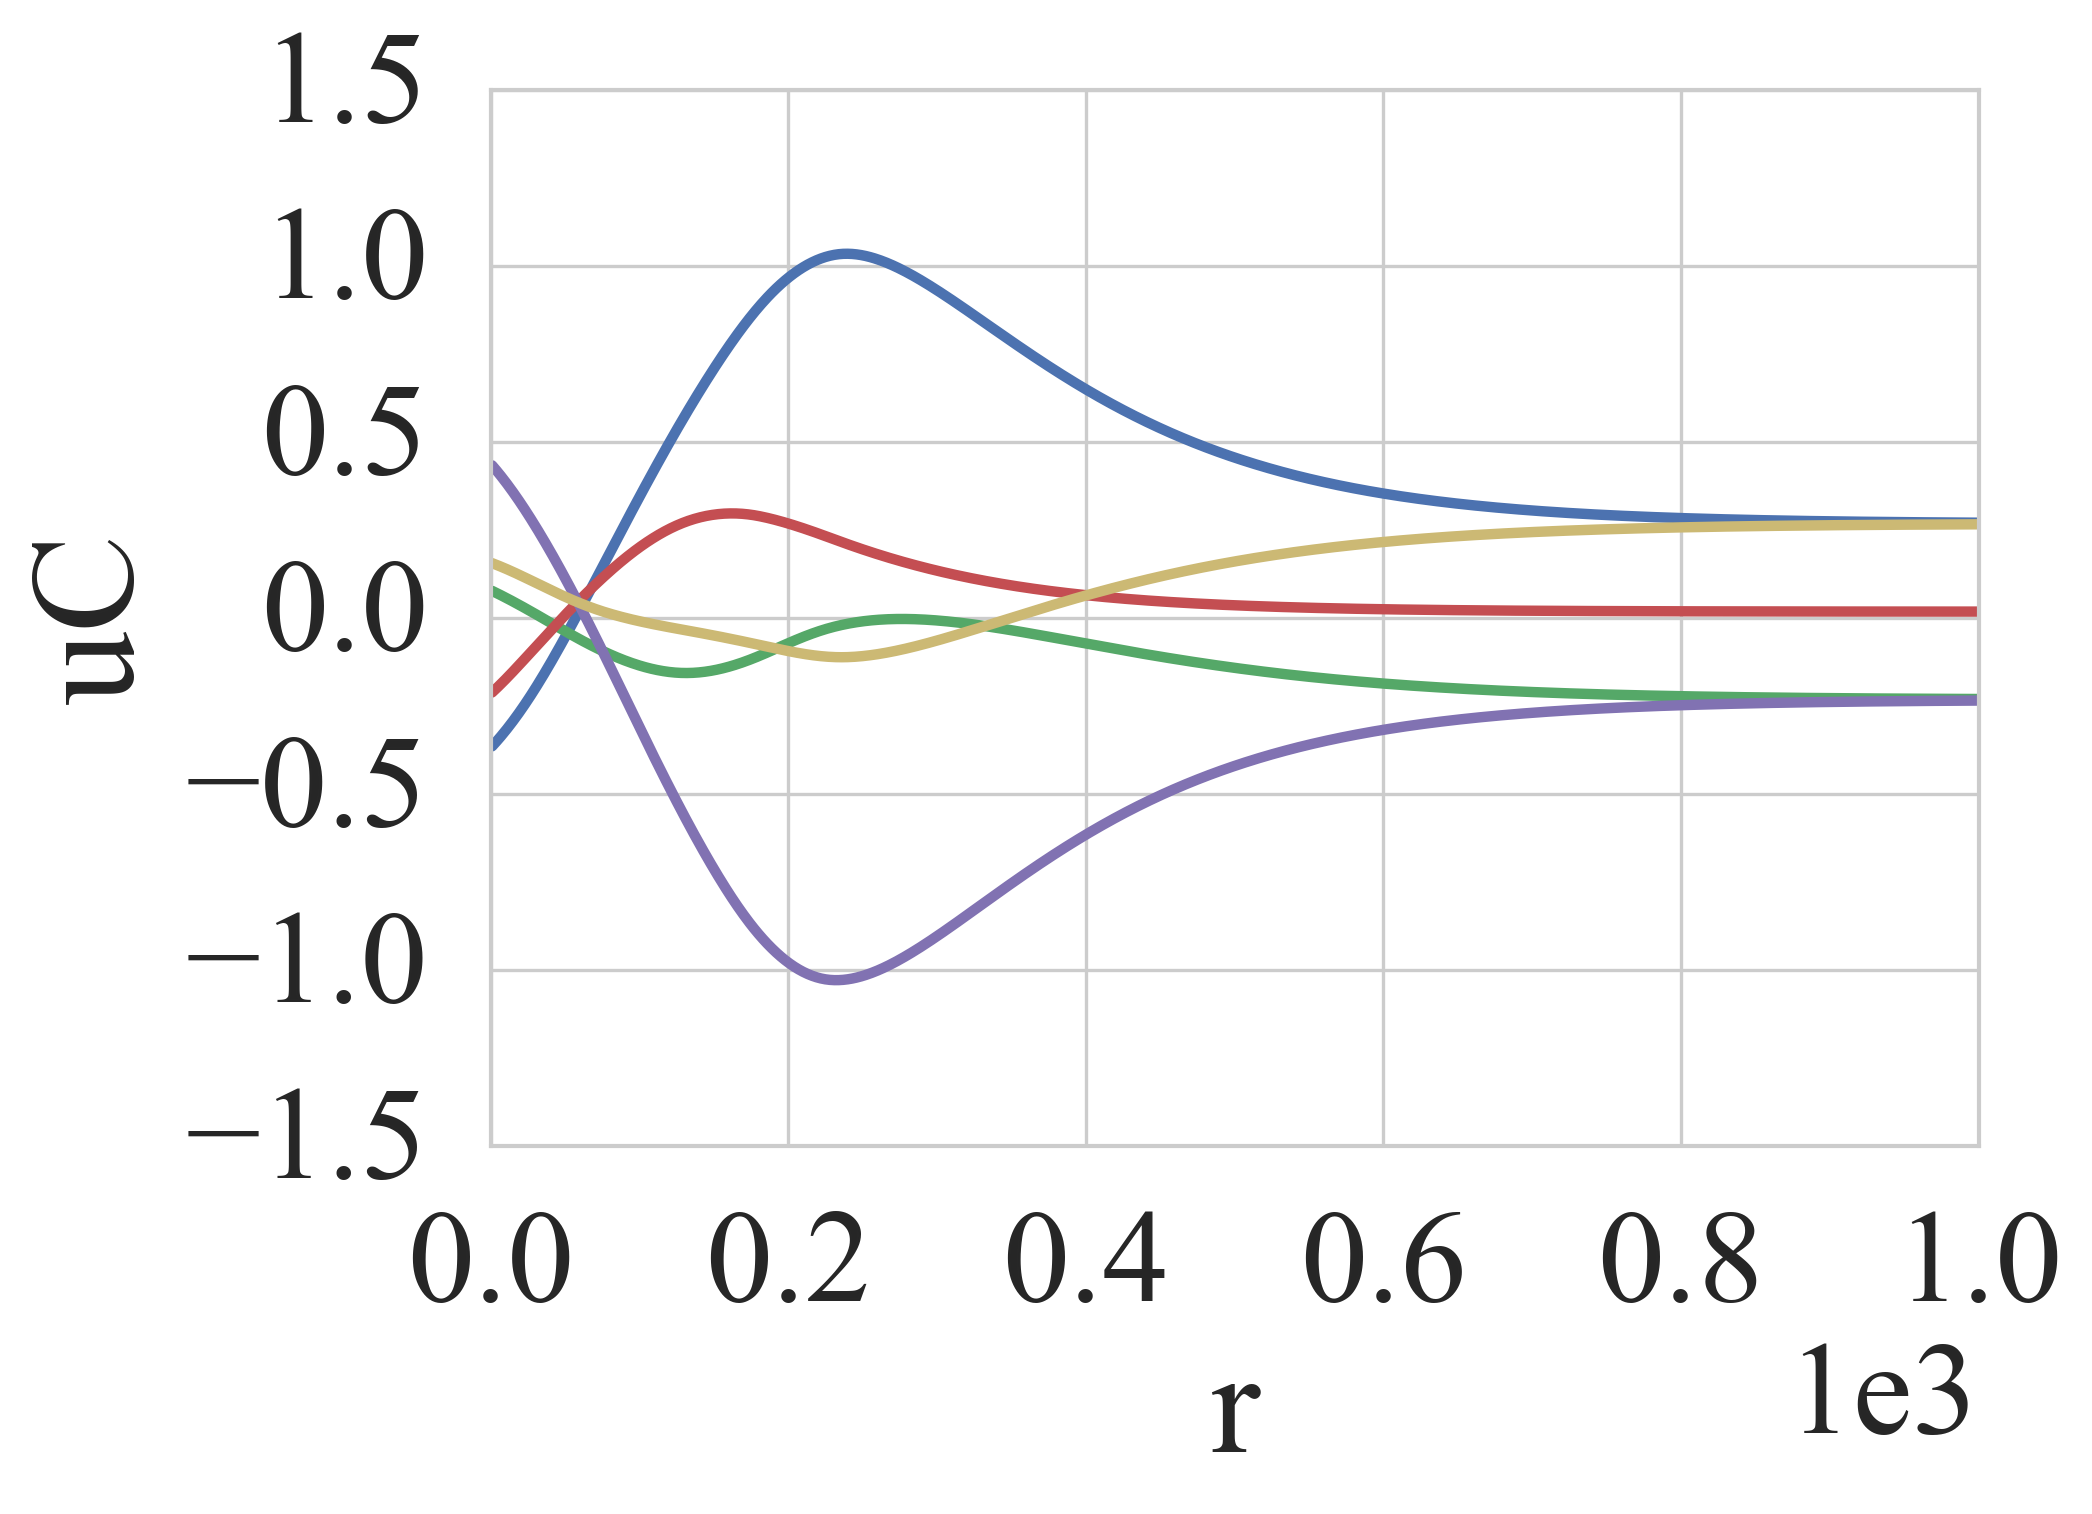
\includegraphics[width=0.4\linewidth,keepaspectratio]{./simulation/diamond/diamond_uC_symmetric_negative.png}\label{fig:diamond_uC_symmetric_negative}}
			\newline
			\subfloat[][]{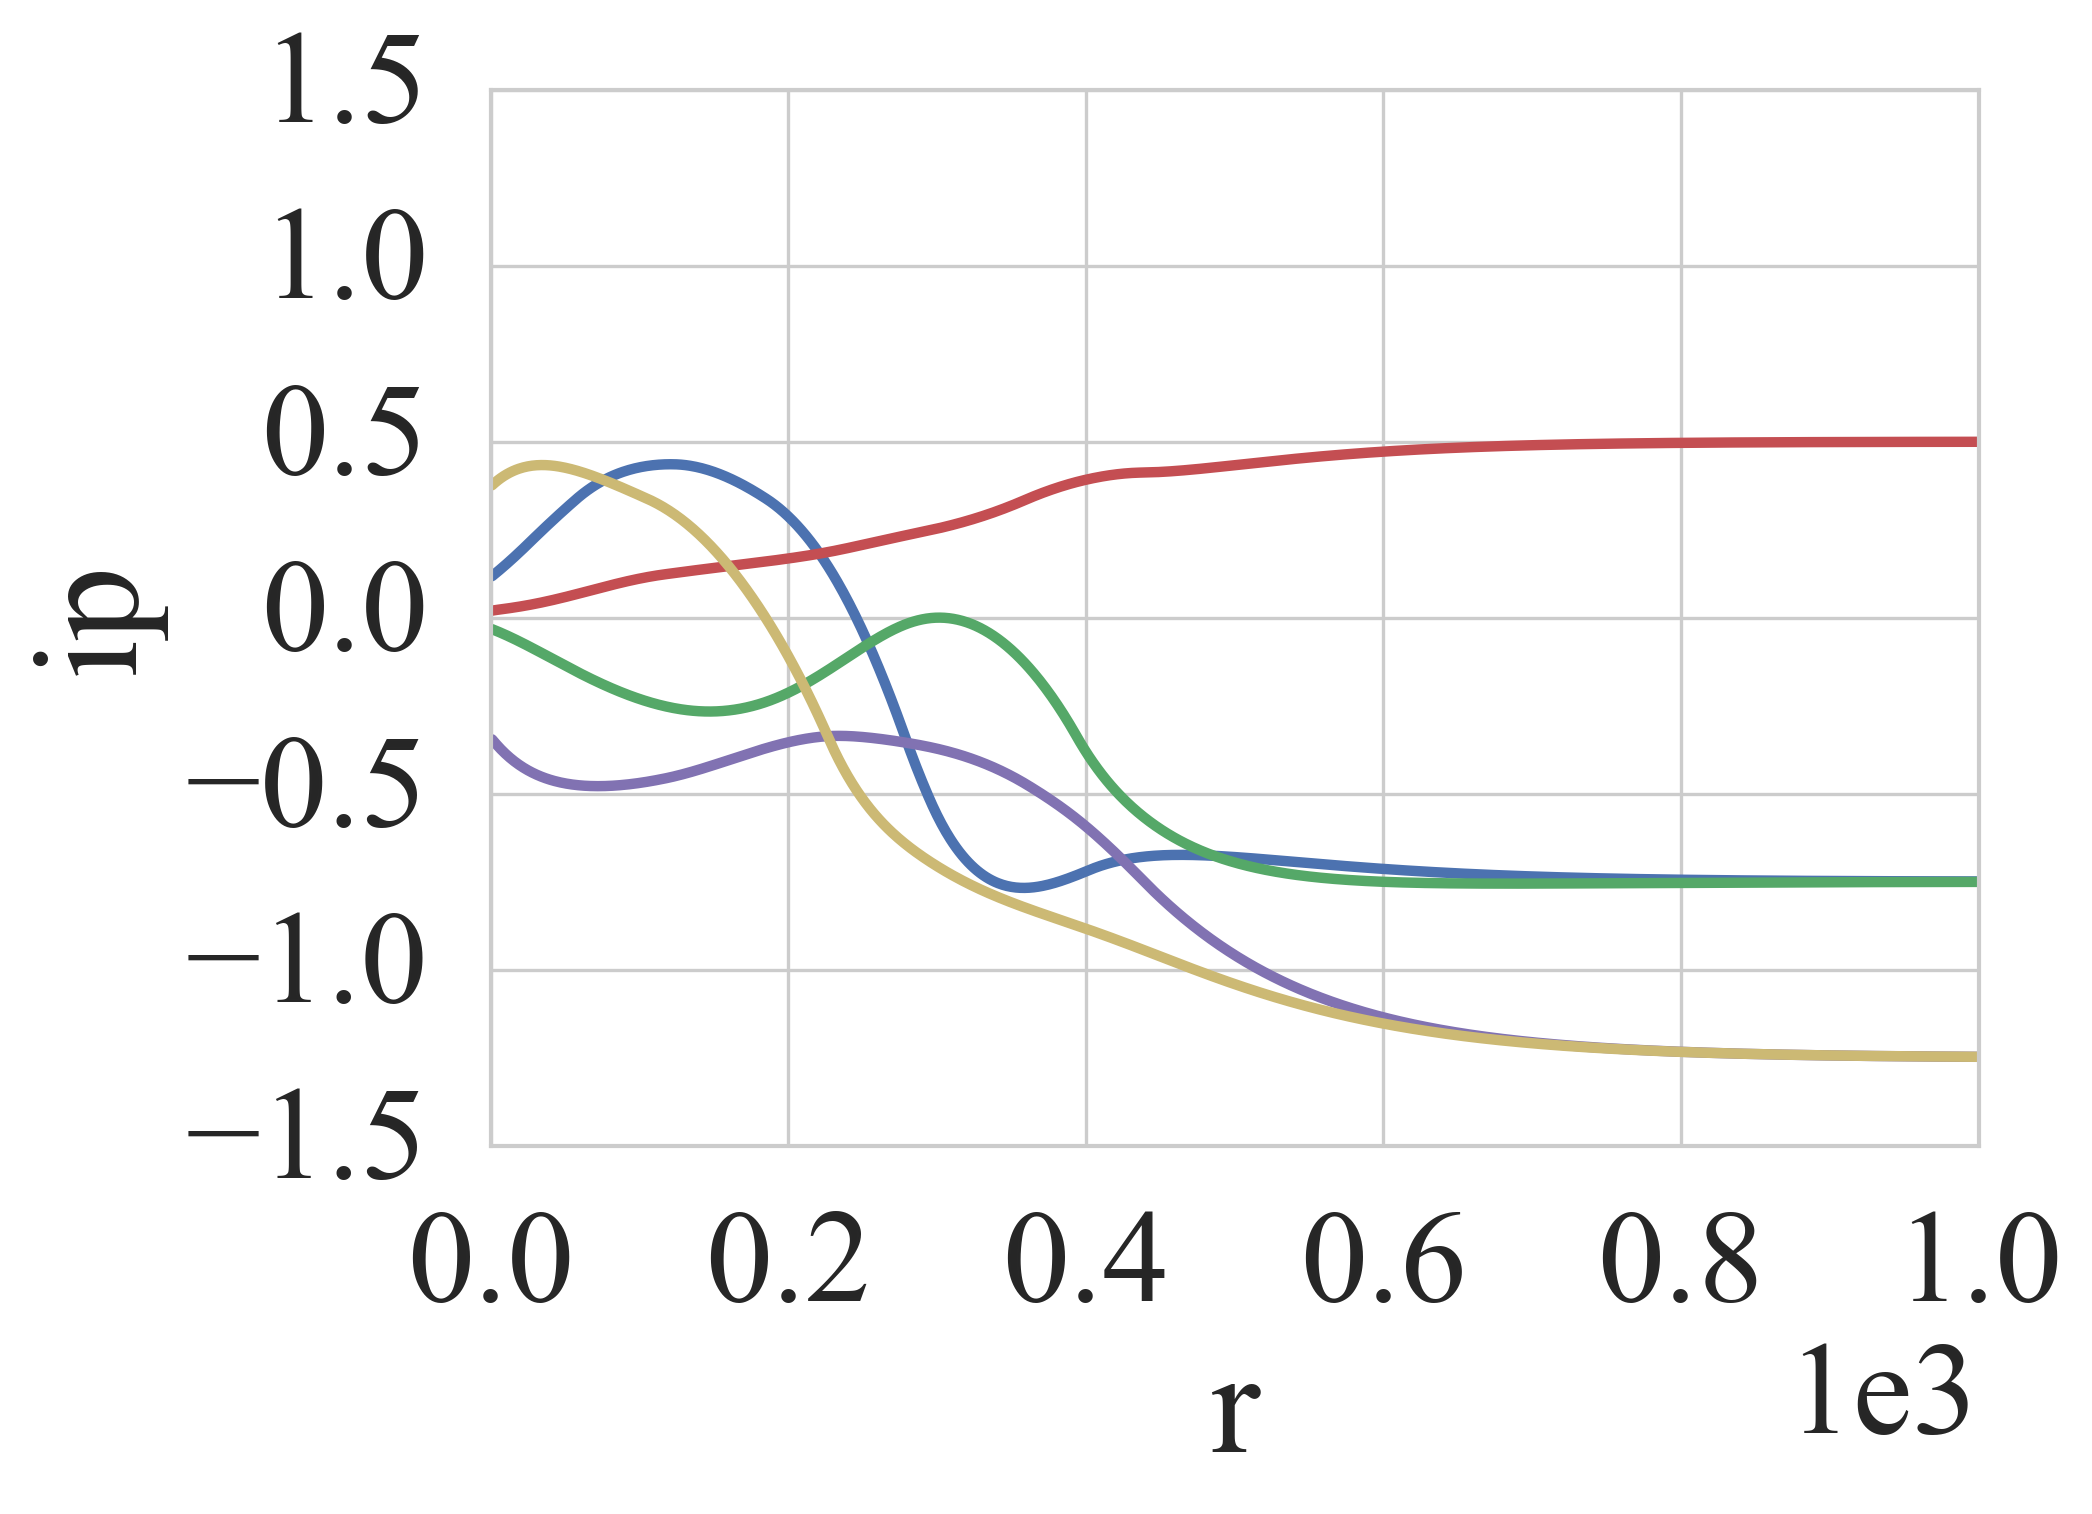
\includegraphics[width=0.4\linewidth,keepaspectratio]{./simulation/diamond/diamond_ip_asymmetric_positive.png}\label{fig:diamond_ip_asymmetric_positive}}\qquad
			\subfloat[][]{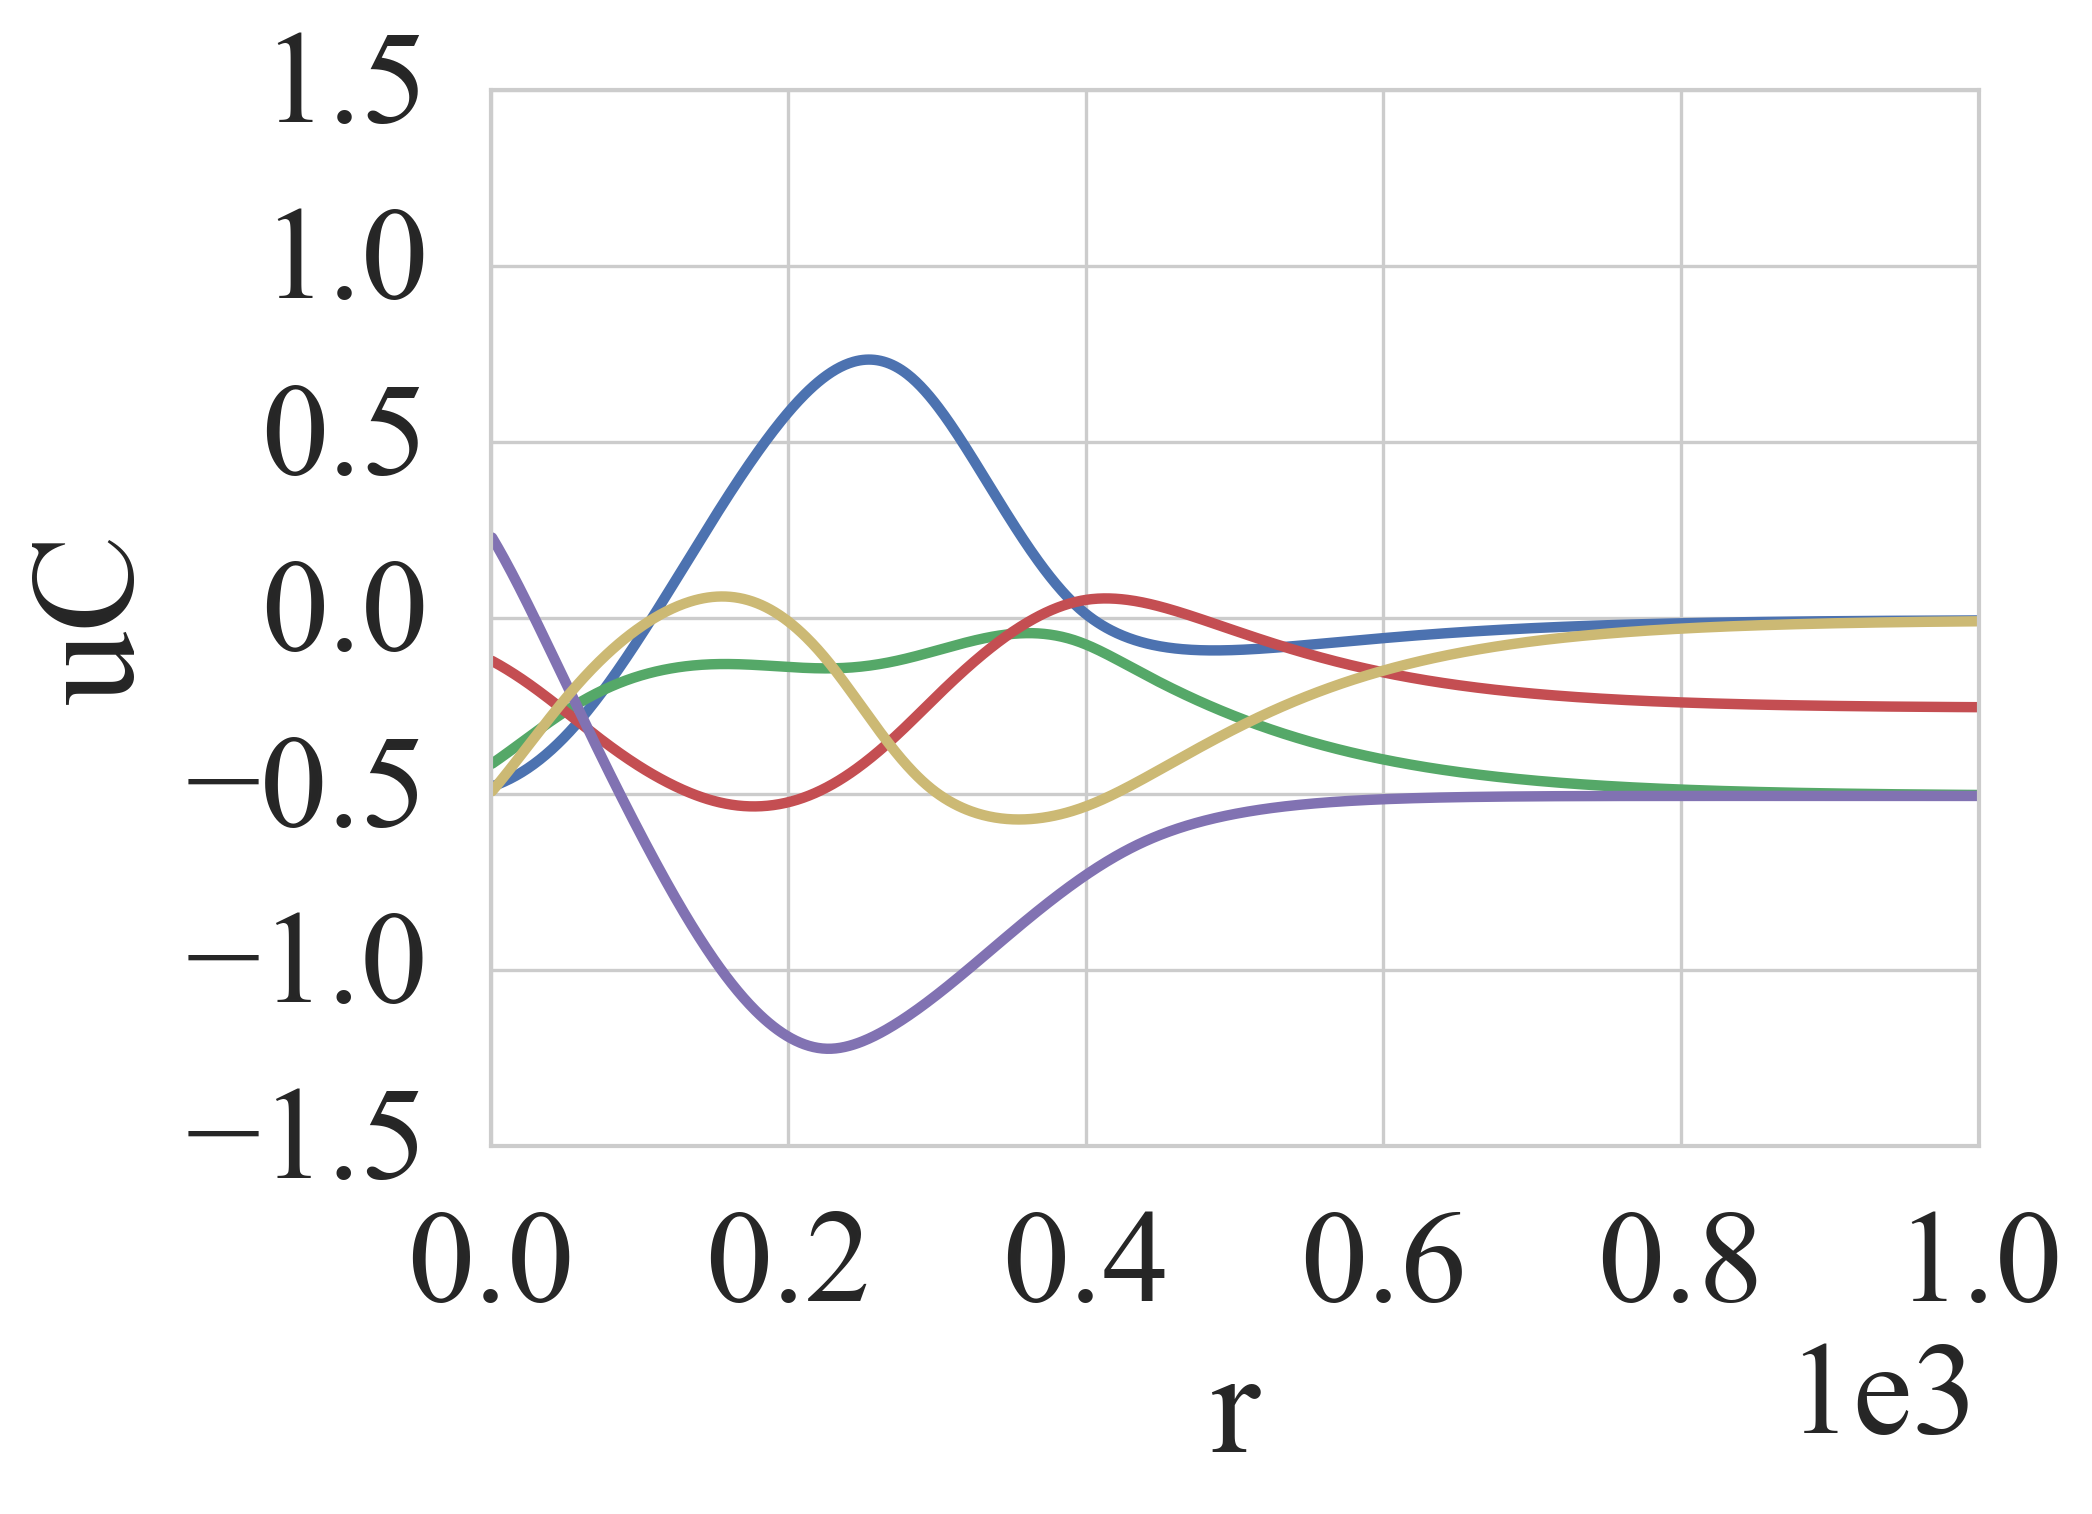
\includegraphics[width=0.4\linewidth,keepaspectratio]{./simulation/diamond/diamond_uC_asymmetric_positive.png}\label{fig:diamond_uC_asymmetric_positive}}
			
			\caption[Path simulations]{Diamond of \Pes.}
			\label{fig:diamond}
		\end{figure}


	\subsection{Paths of \emph{Physarum} Elements}

		Next we look at paths of \Pes. Here no circulation is possible but neighboring \Pes still interact with each other leading to non-zero currents. \Fref{fig:path_5} depicts a path consisting of $5$ chained \Pes. Again \Fref{fig:path_5_legend} defines a color coding which serves as a legend for the remaining plots of \Fref{fig:paths}. We show the results of three different sub-path of \Fref{fig:path_5} starting at node $0$. The paths have lengths $l \in [2,3,4]$.

		First, note the capacitor voltages of at least one edge does not converge for any of the depicted paths, see \Fref{fig:path_3_uC}, \Fref{fig:path_4_uC} and \Fref{fig:path_5_uC}. All most all voltages are quasi-periodic and thus none of these \Pes are converged. 

		A similar behavior is observed for the currents illustrated in \Fref{fig:path_3_ip}, \Fref{fig:path_4_ip} as well as \Fref{fig:path_5_ip}. Note that for all paths we find that the currents of all but one edge periodically revers their sign, \ie flow reversal occurs naturally. At present, we do not know why there always remains one edge with zero flow.

		The distinguishing feature of these \Pes seems to be the period of the oscillations. For paths of length $3$ we repeated the simulation $100$ times with different random initial conditions. Without fail the \Pn produced a signal with a period of $T = 1087$ rounds in every execution. We thus conclude that the period is invariant under initial conditions within the ranges we explored. 

		Furthermore, we find that the period of the oscillations decreases with increasing path length. For small path lengths the observed values suggest a linear relation between path length and period as a best fit. To explore the matter further we extended the simulations to paths lengths of up to $10$. We found that a simple functional relationship between path length and period cannot be confirmed of all tested lengths. Rather, for path lengths longer than $7$, more complicated oscillation patters are found to repeat themselves. Here it appears that higher order oscillations come into play. At present their meaning is not clear to the authors. We conclude, however, that there is complex relation between the oscillation patterns and the size of the underlying \Pes that warrants further exploration.

		Another aspect waiting to be investigated for the first time is the nature of the phase shifts observed between the edges of the circuits. 
                
		\begin{figure}
			\centering
			\subfloat[][]{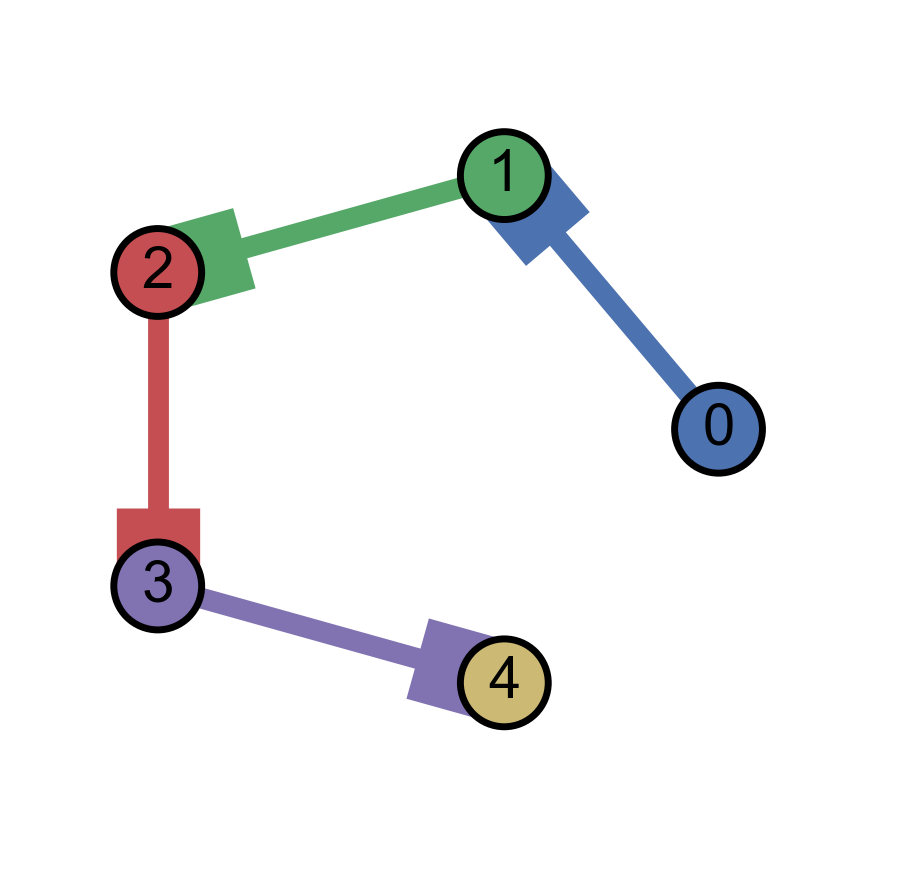
\includegraphics[width=0.4\linewidth,keepaspectratio,trim={0 3cm 0 3cm},clip]{./simulation/path/path_5.png}\label{fig:path_5}}\qquad
			\subfloat[][]{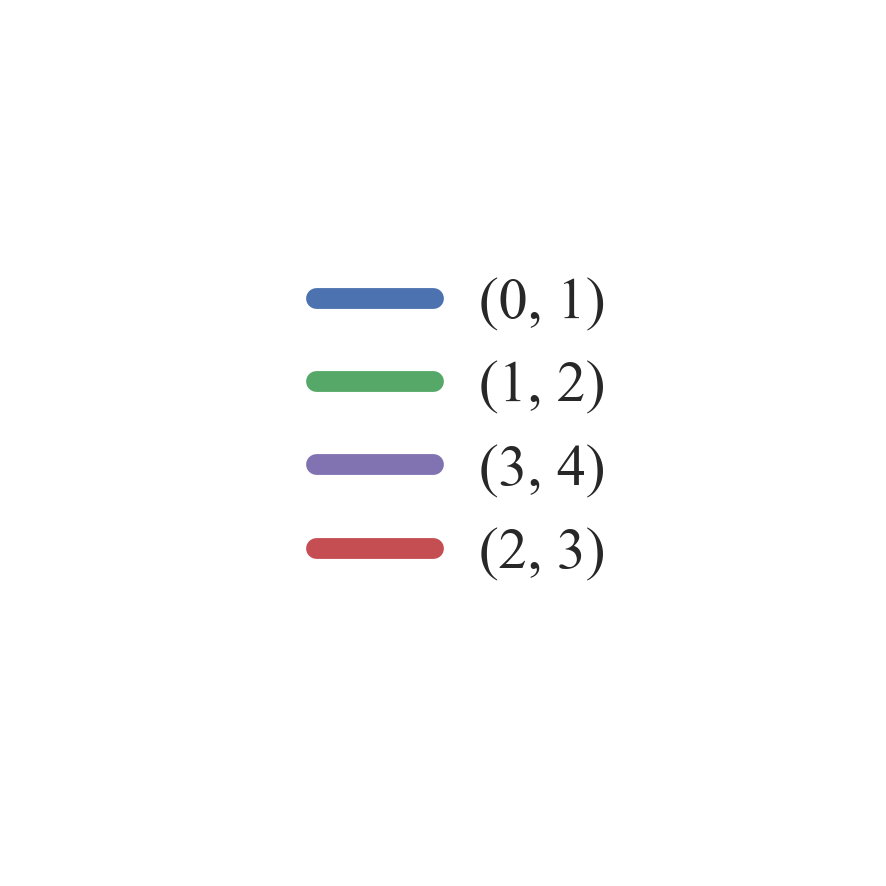
\includegraphics[width=0.4\linewidth,keepaspectratio,trim={0 3cm 0 3cm},clip]{./simulation/path/path_5_legend.png}\label{fig:path_5_legend}}
			\newline
			\subfloat[][Period $T \approx 694$ rounds.]{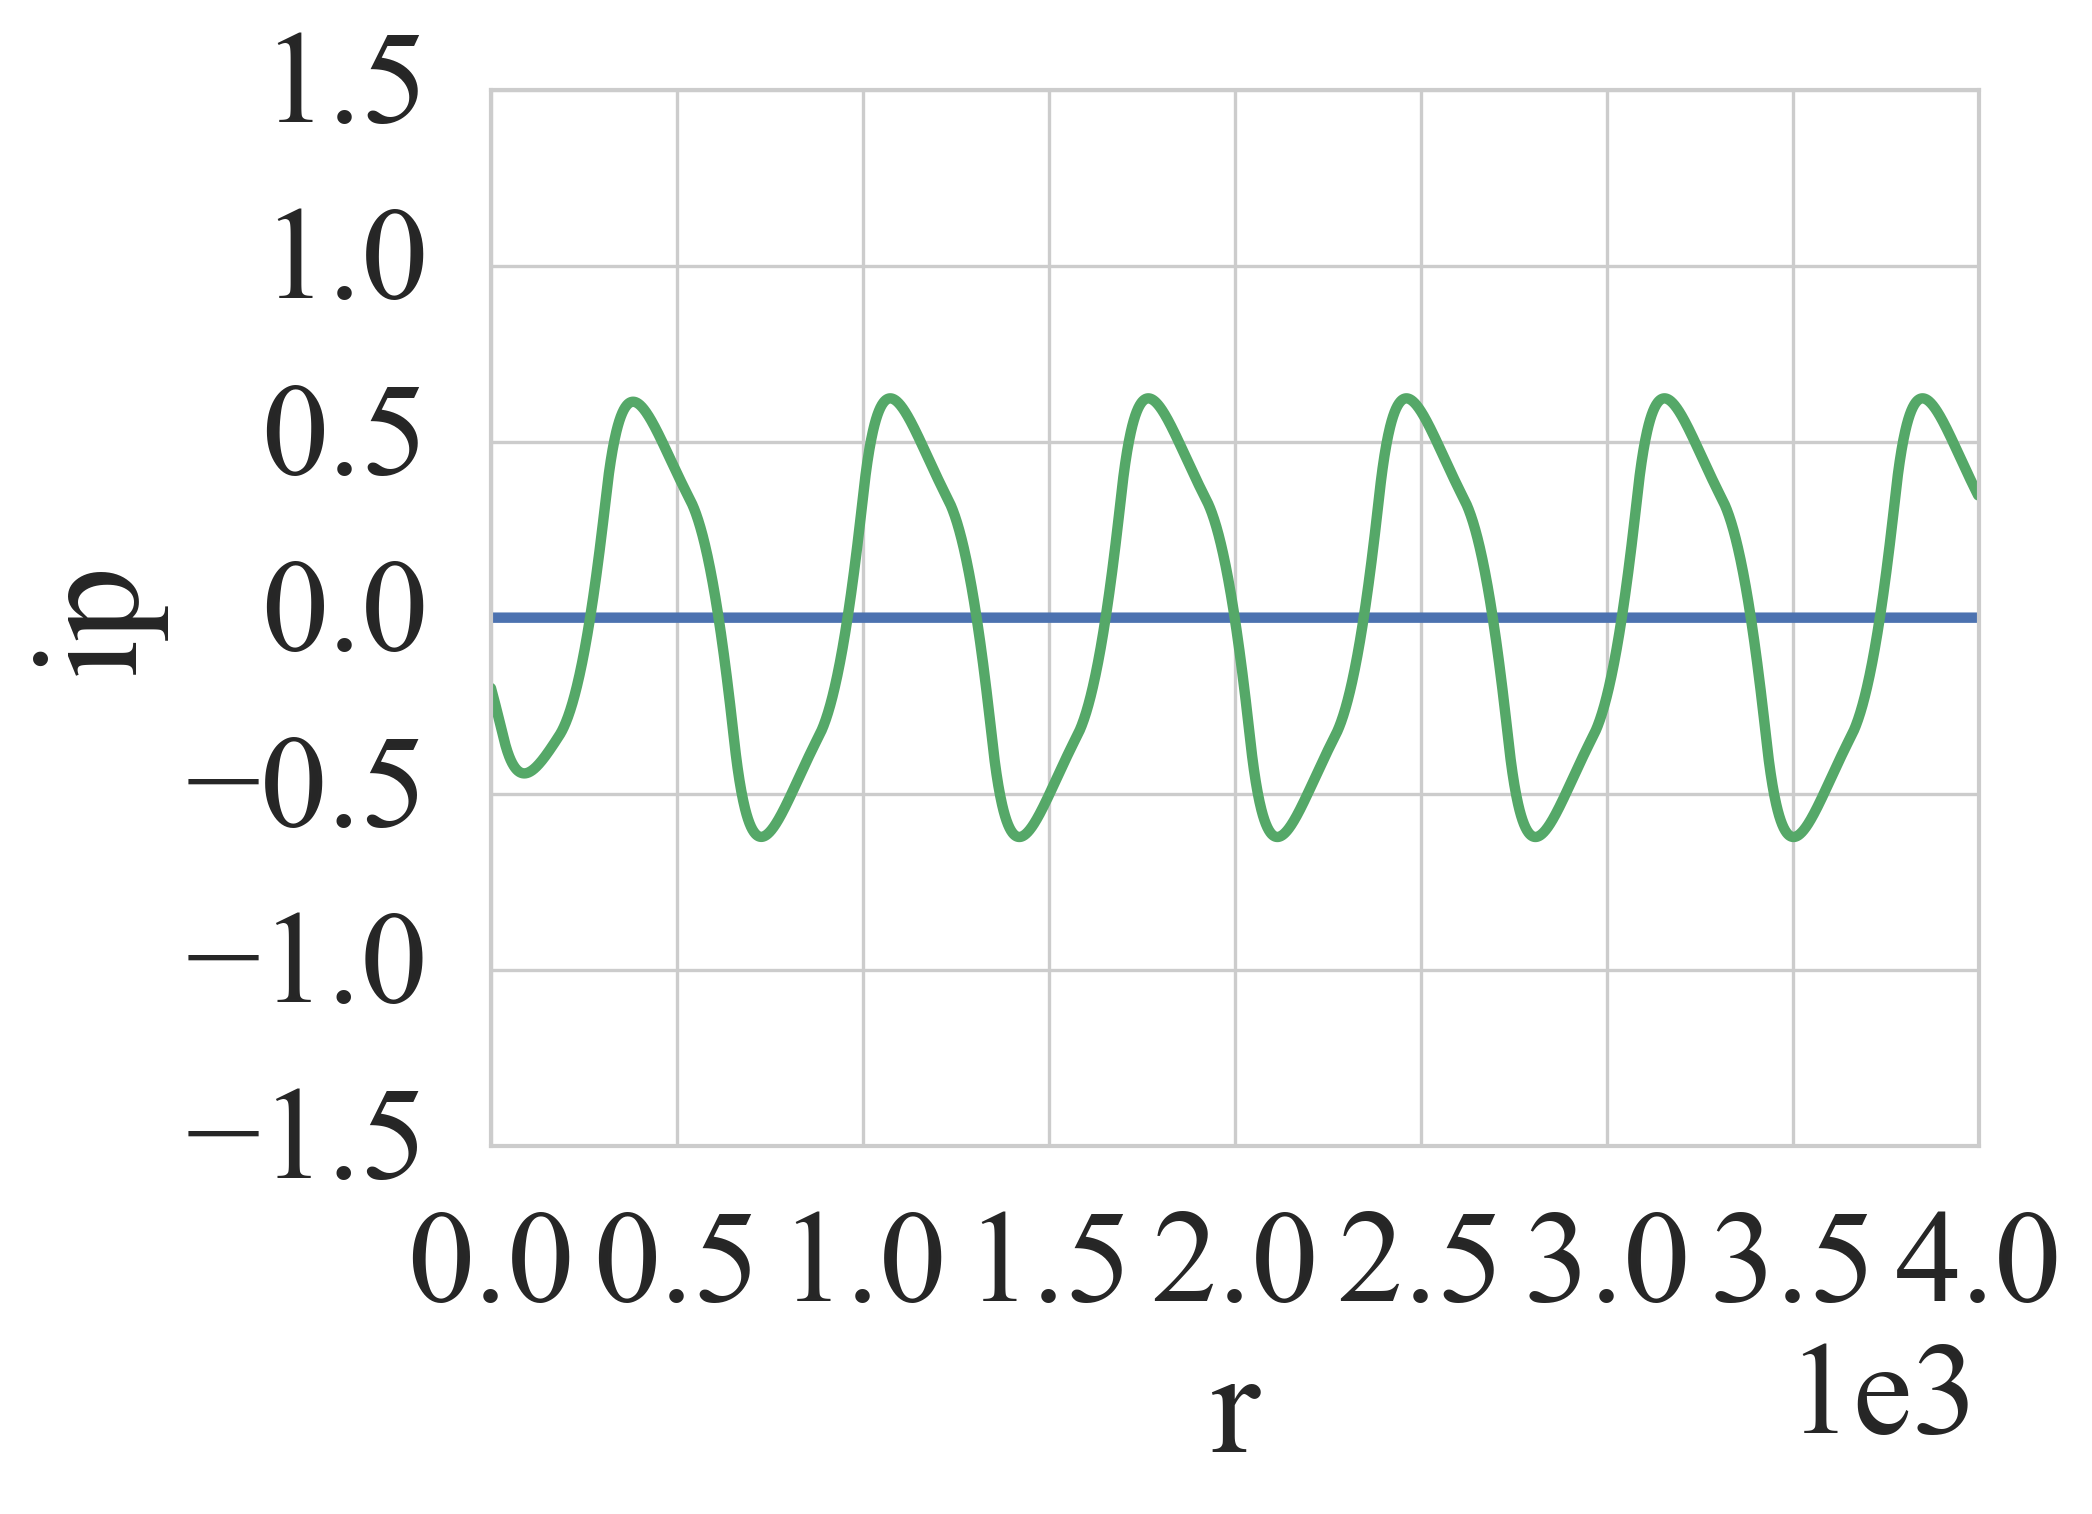
\includegraphics[width=0.4\linewidth,keepaspectratio]{./simulation/path/path_3_ip.png}\label{fig:path_3_ip}}\qquad
			\subfloat[][Period $T \approx 694$ rounds.]{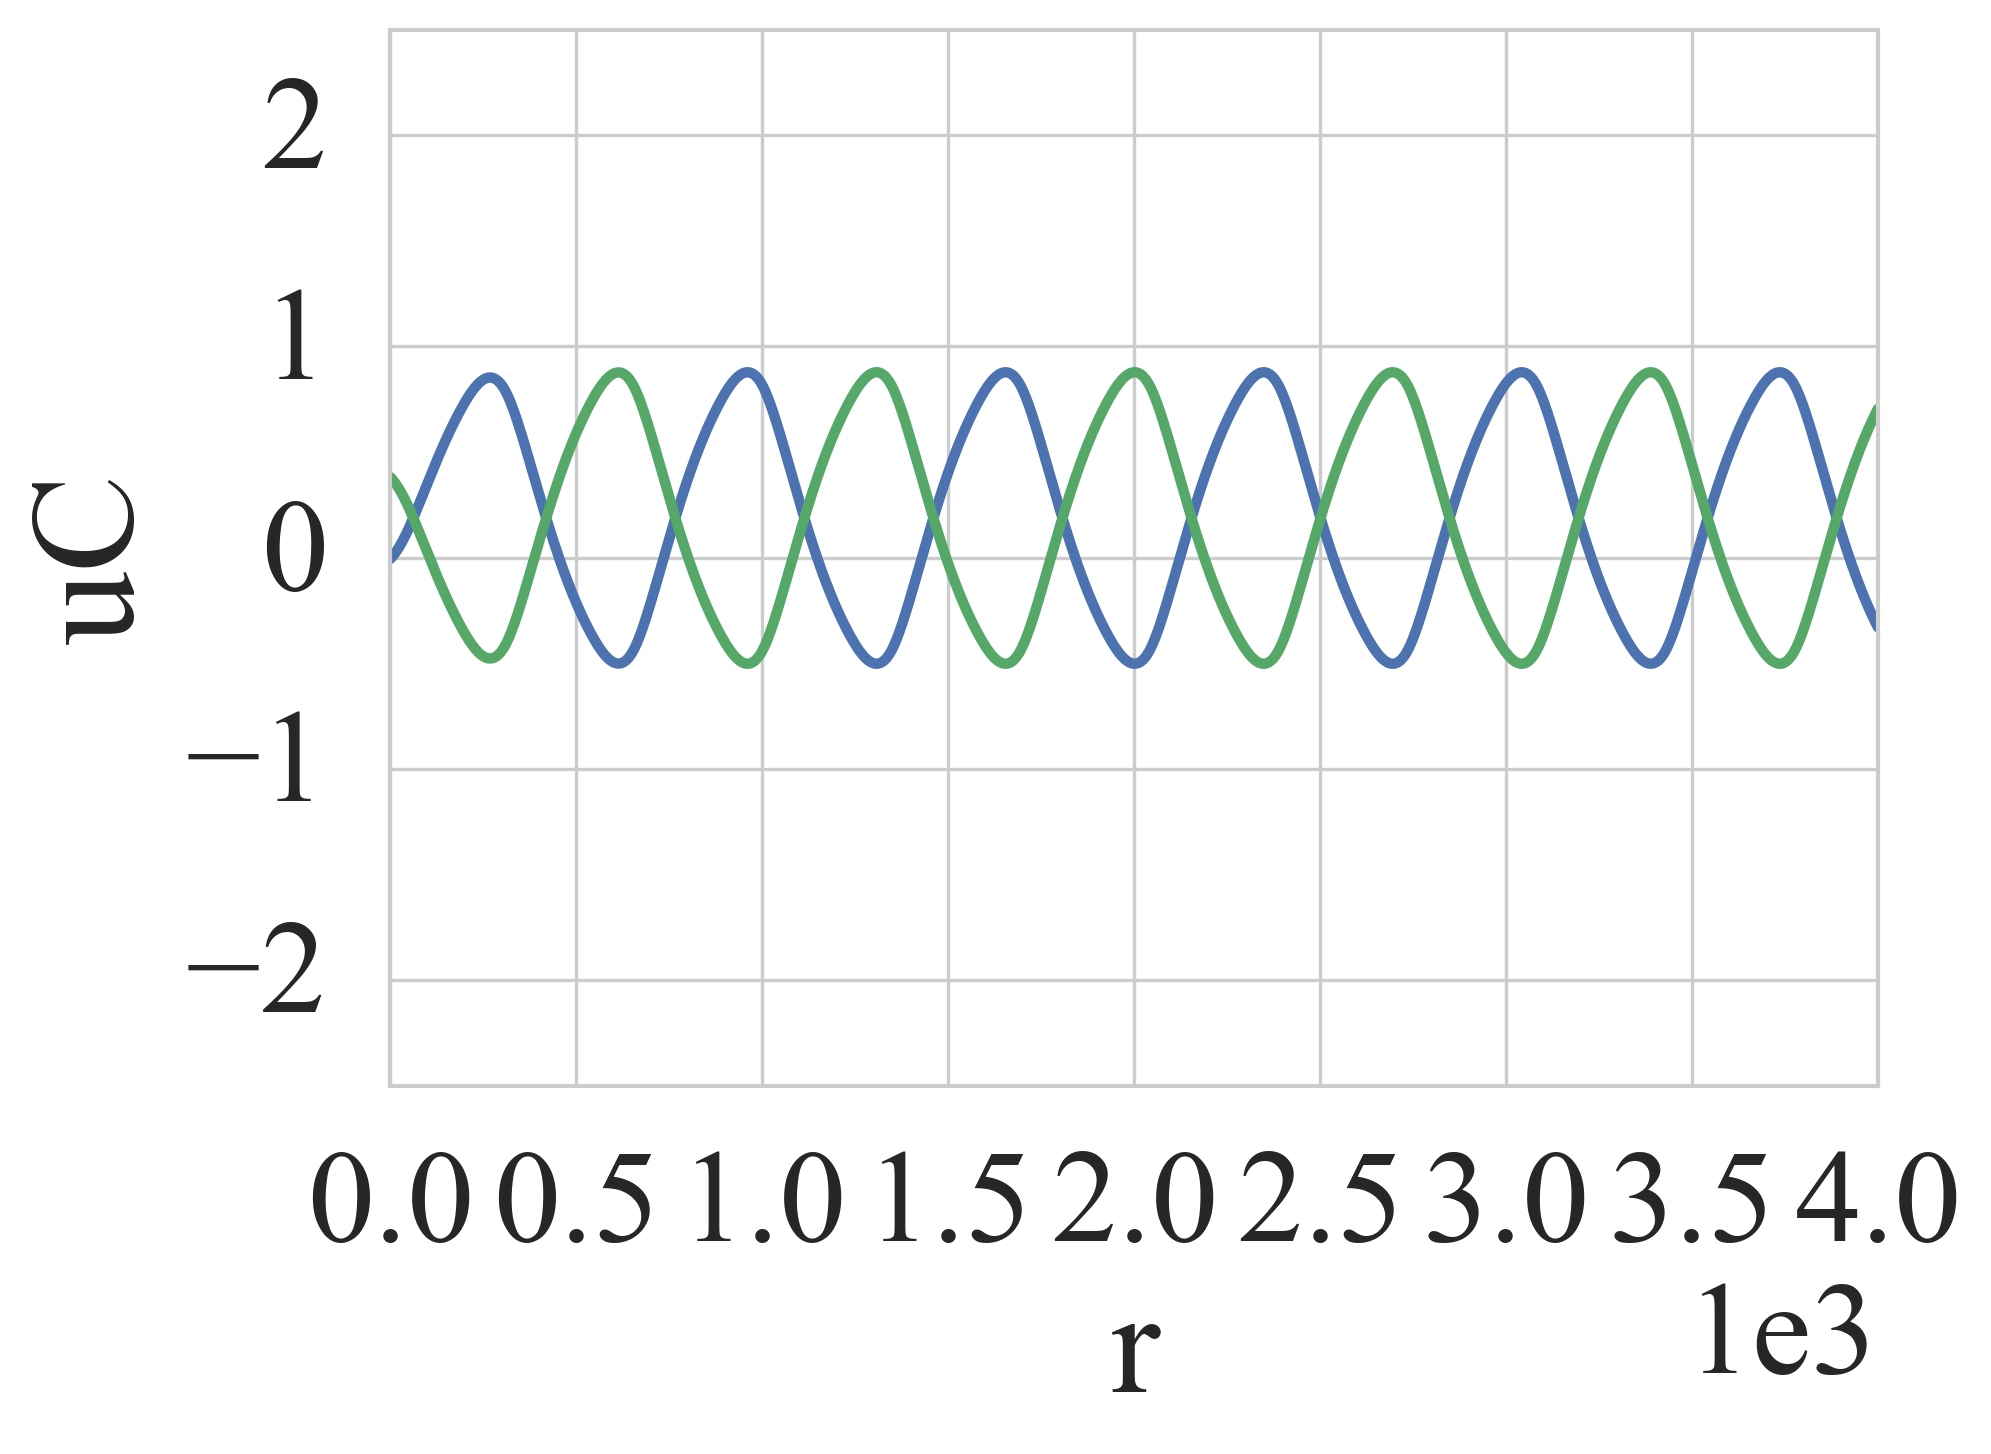
\includegraphics[width=0.4\linewidth,keepaspectratio]{./simulation/path/path_3_uC.png}\label{fig:path_3_uC}}
			\newline
			\subfloat[][Period $T \approx 1087$ rounds.]{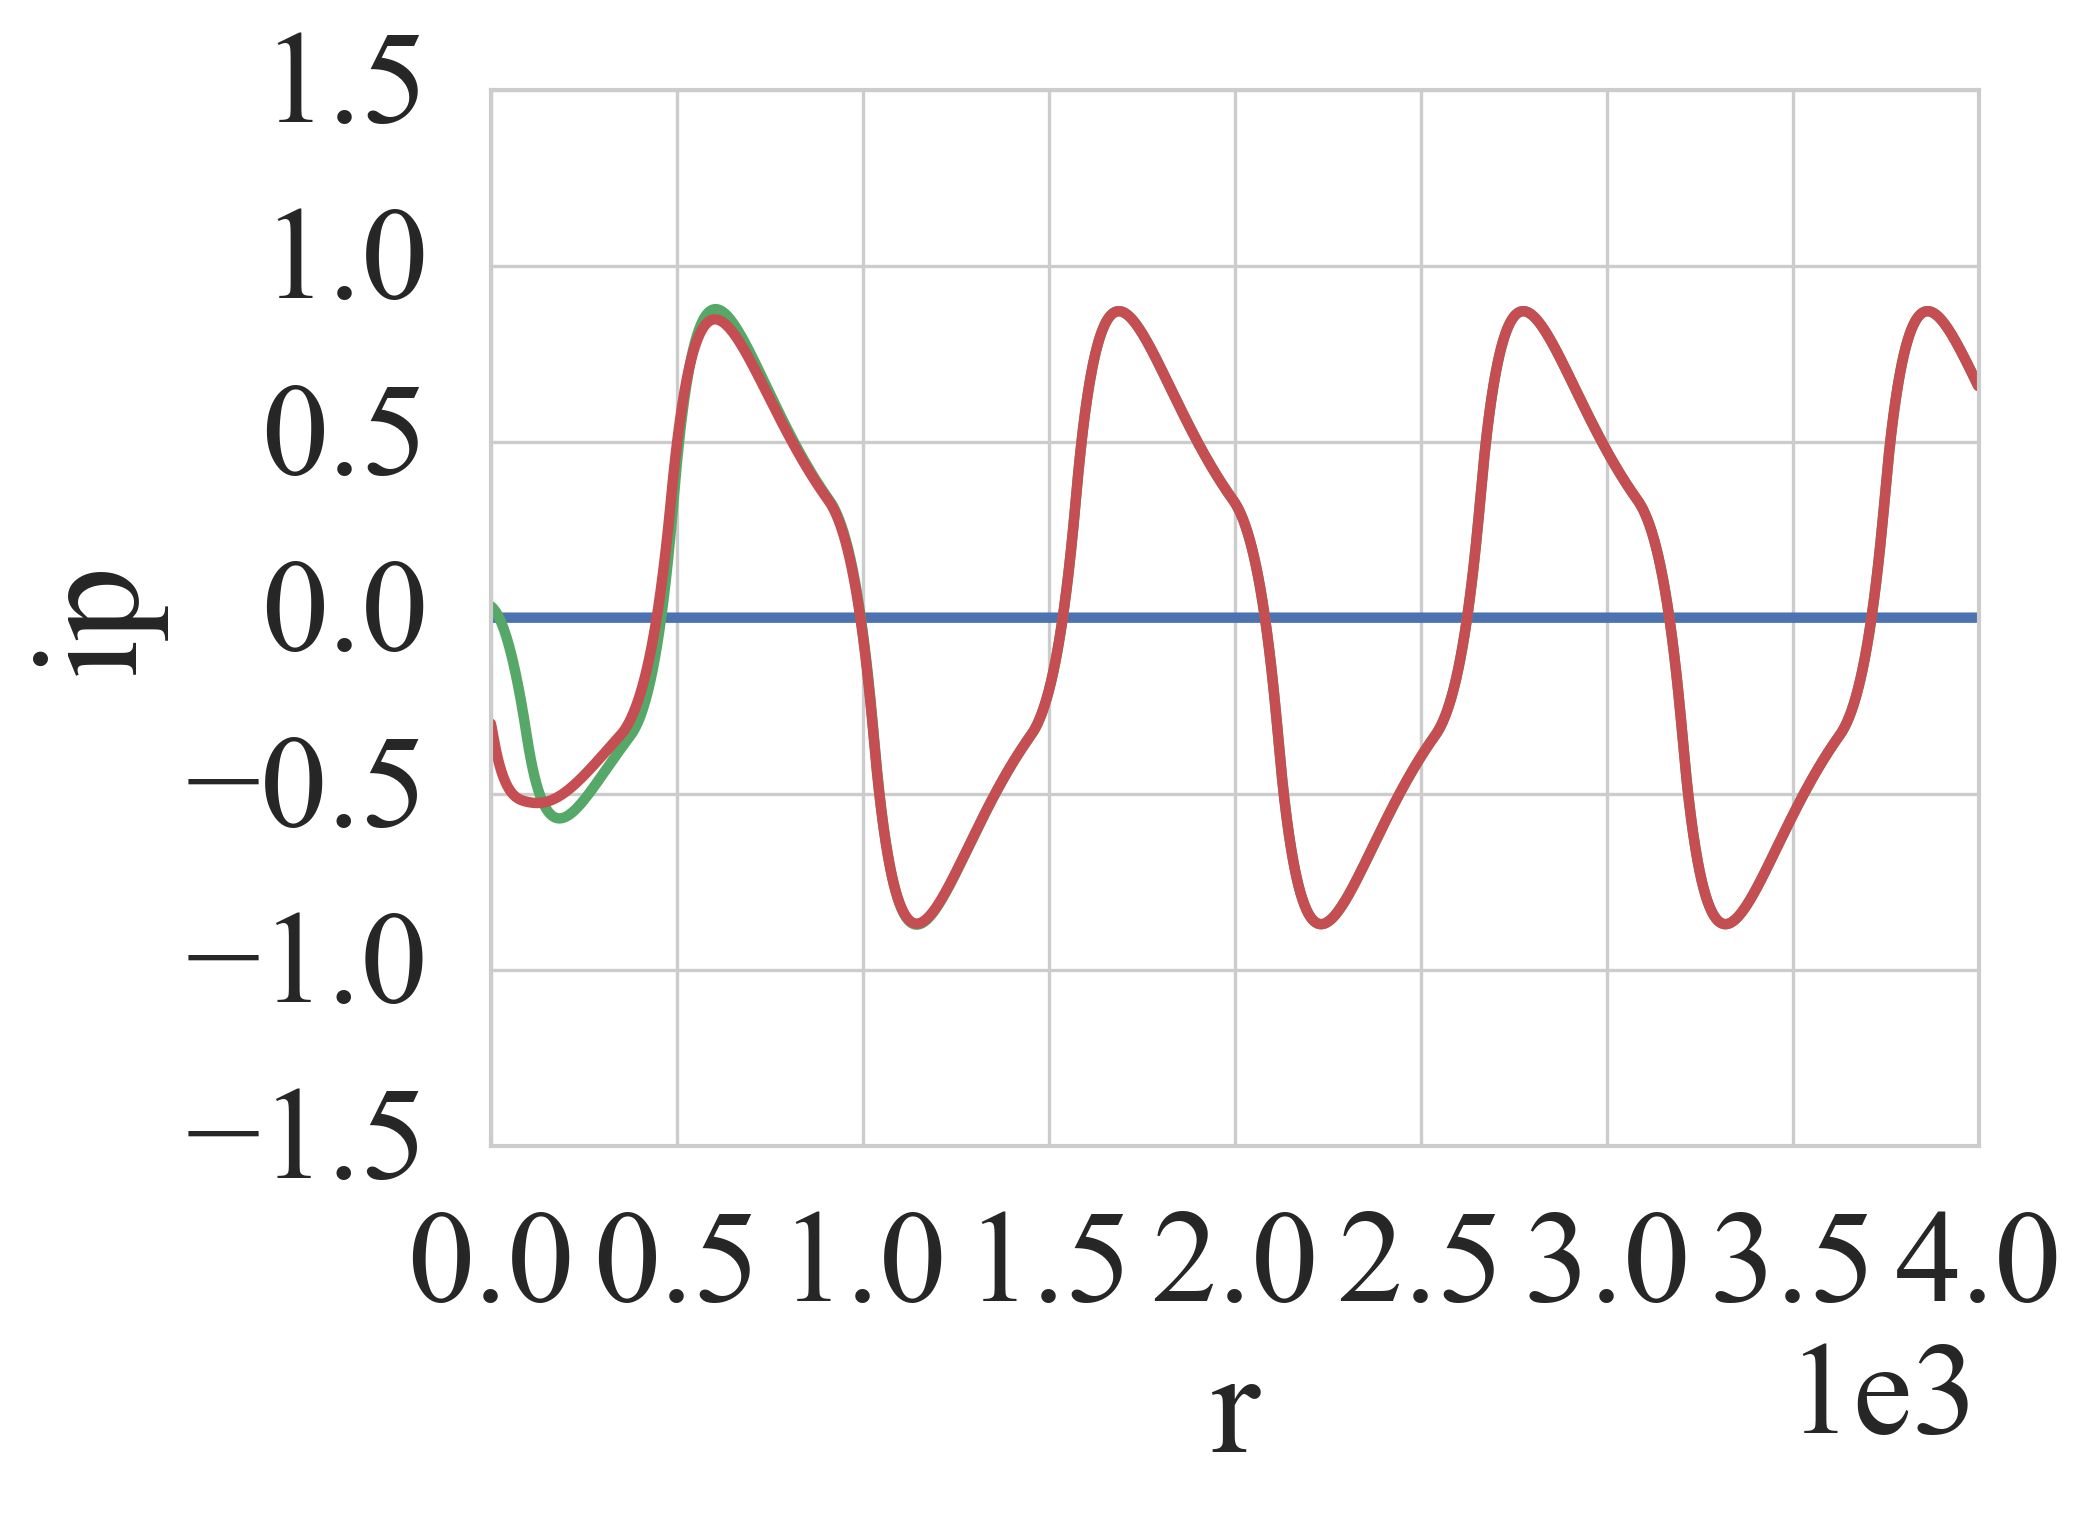
\includegraphics[width=0.4\linewidth,keepaspectratio]{./simulation/path/path_4_ip.png}\label{fig:path_4_ip}}\qquad
			\subfloat[][Period $T \approx 1087$ rounds.]{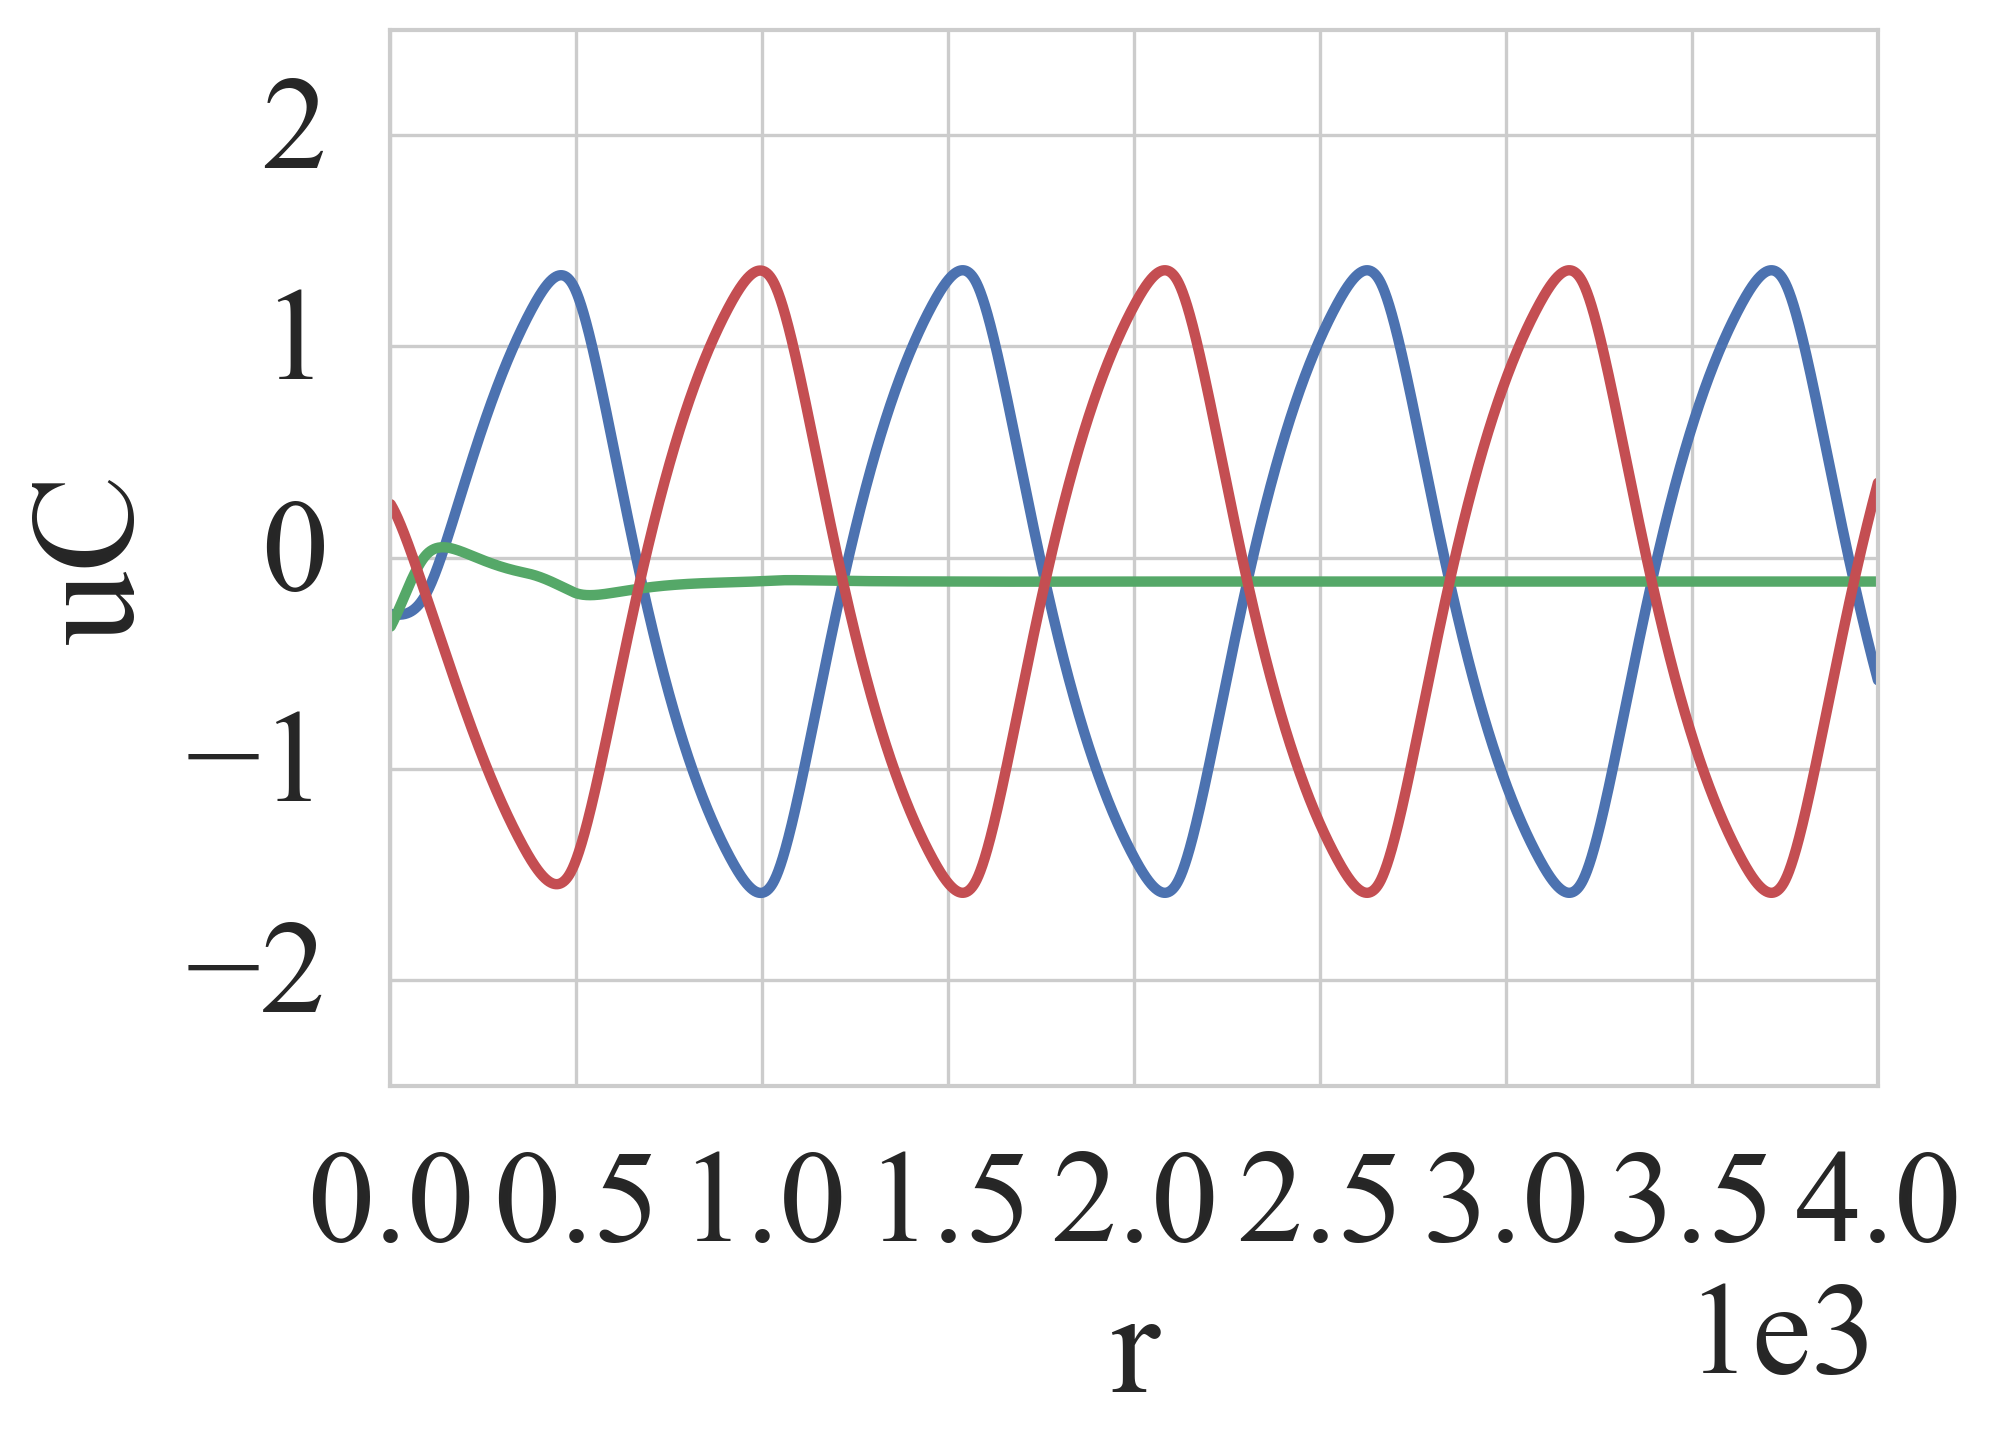
\includegraphics[width=0.4\linewidth,keepaspectratio]{./simulation/path/path_4_uC.png}\label{fig:path_4_uC}}
			\newline
			\subfloat[][Period $T \approx 1522$ rounds.]{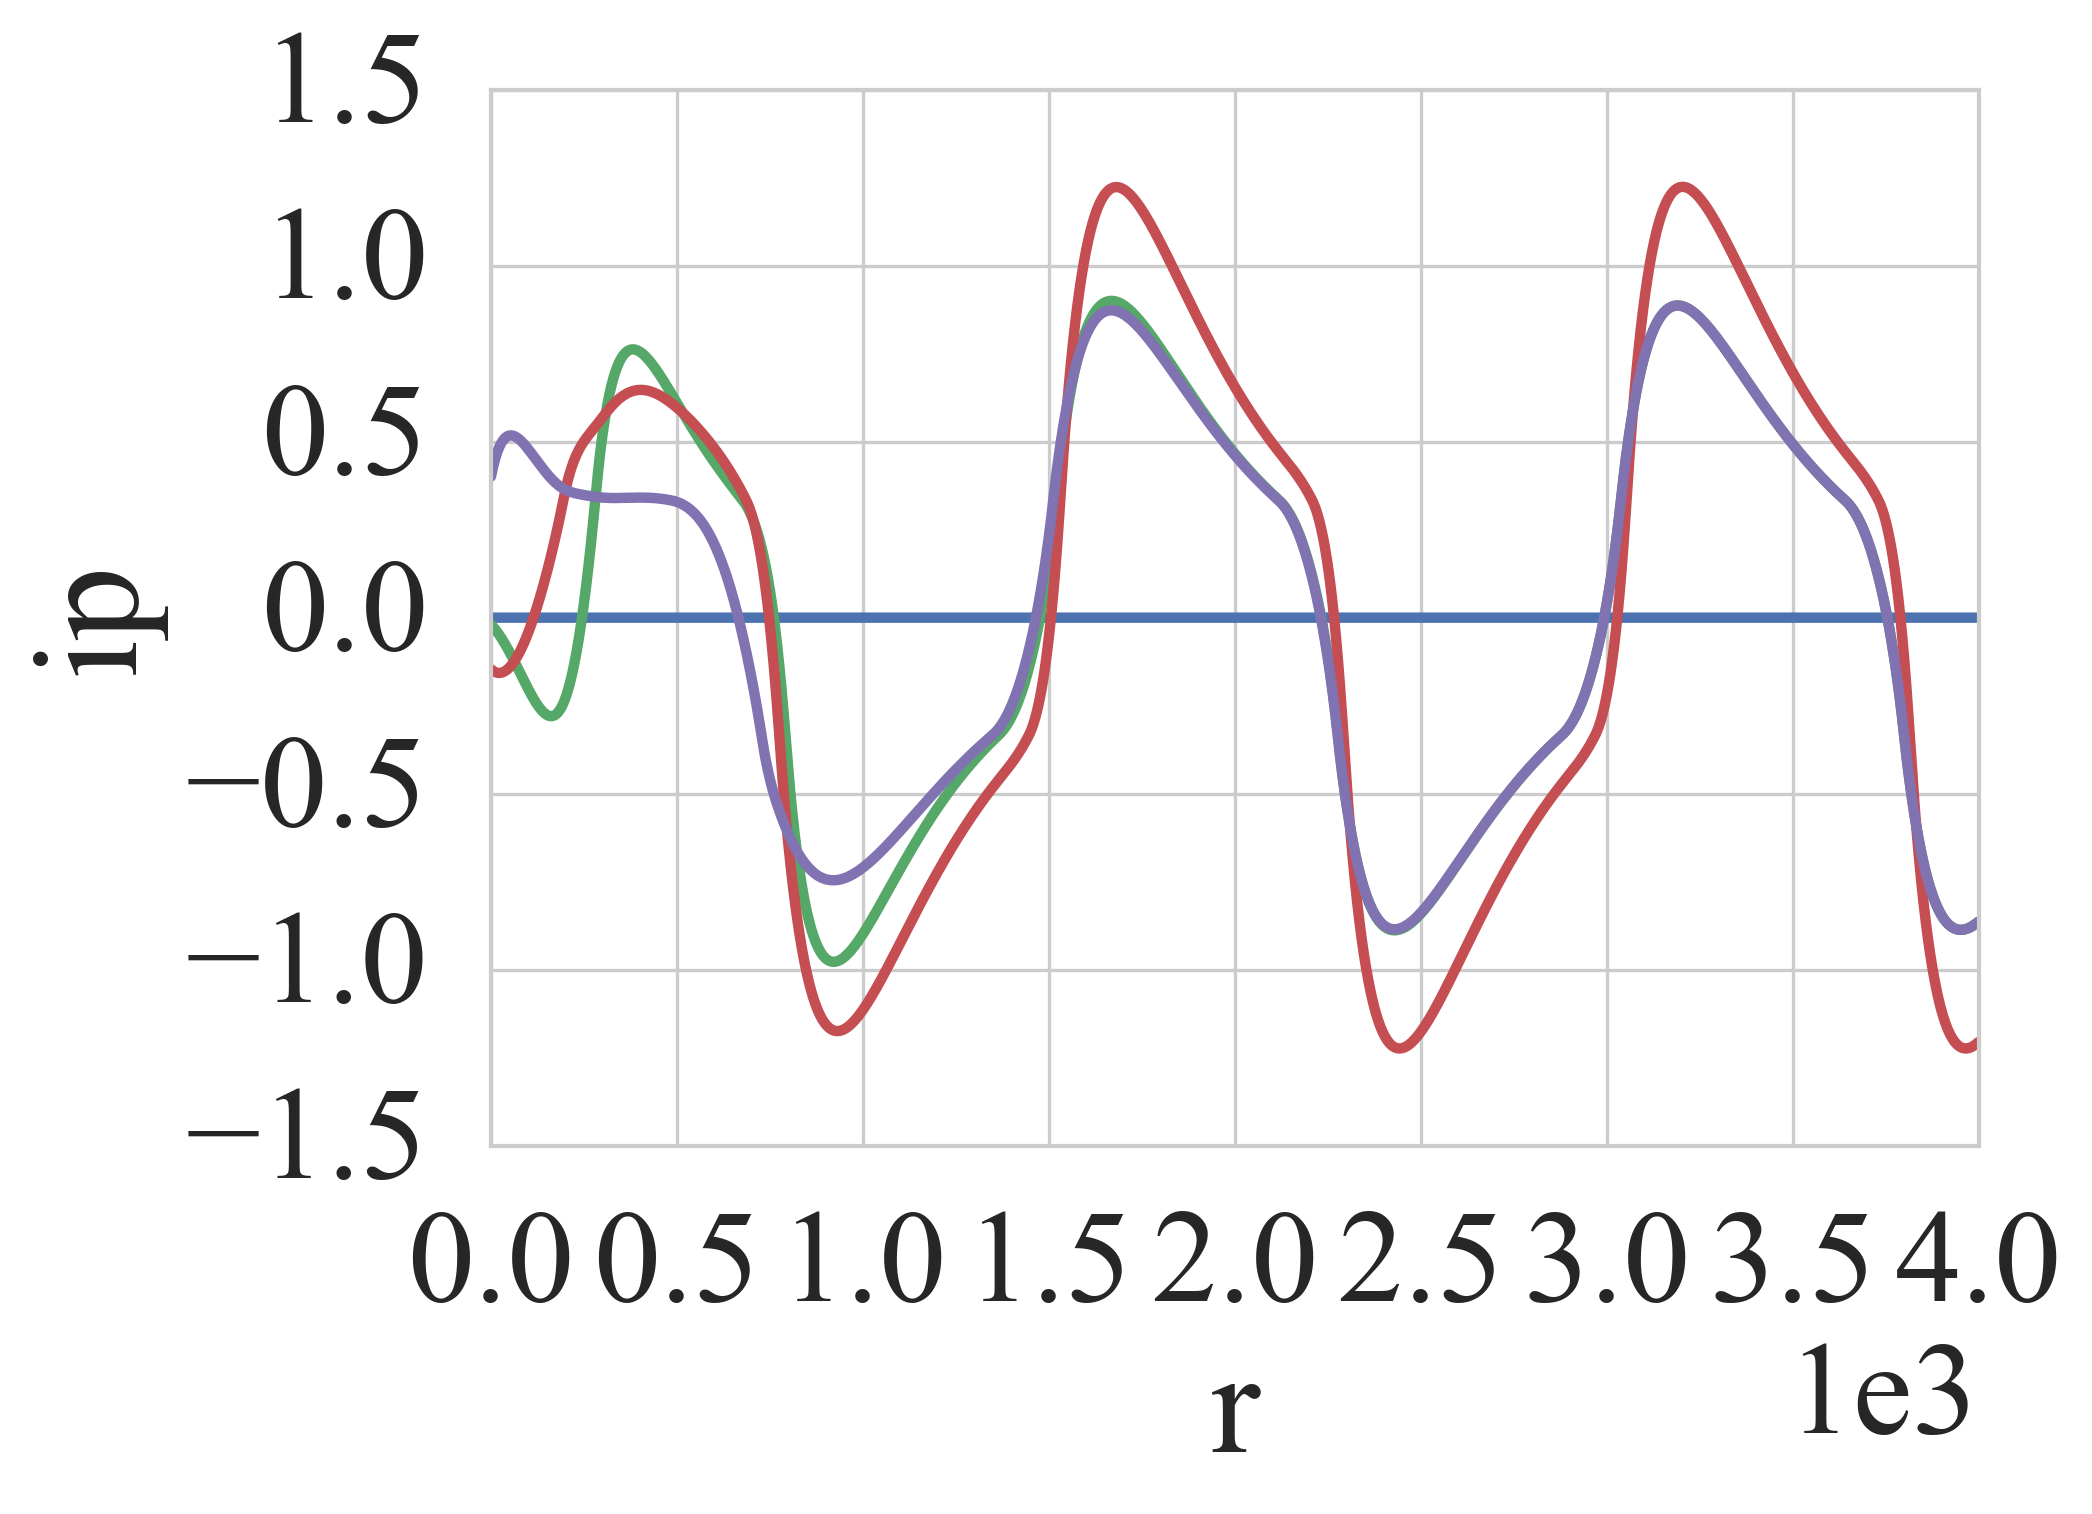
\includegraphics[width=0.4\linewidth,keepaspectratio]{./simulation/path/path_5_ip.png}\label{fig:path_5_ip}}\qquad
			\subfloat[][Period $T \approx 1522$ rounds.]{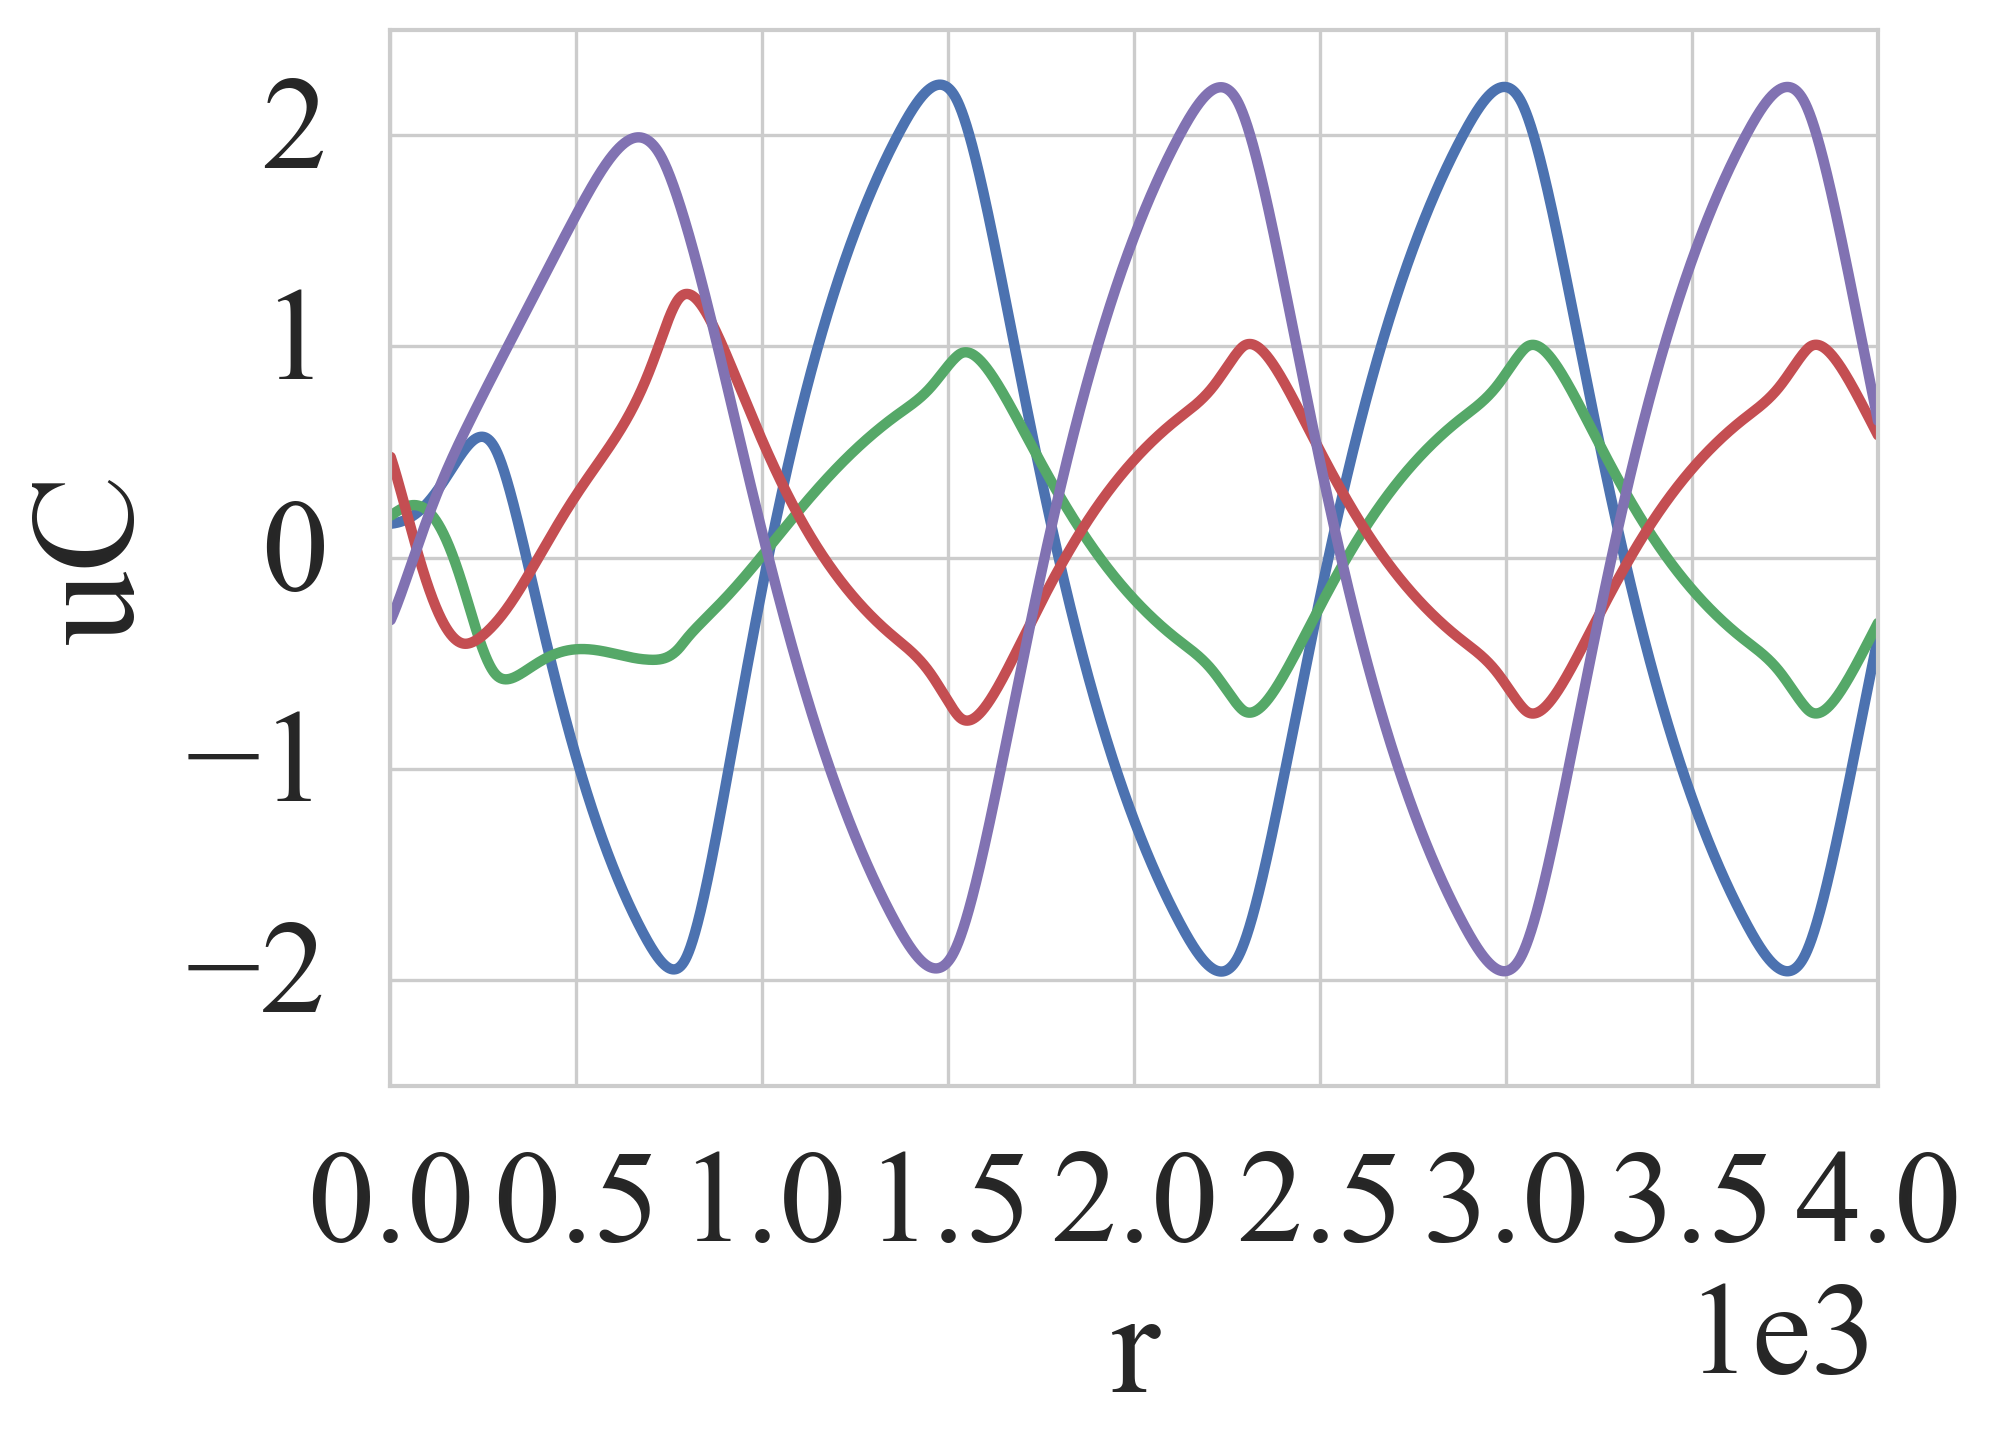
\includegraphics[width=0.4\linewidth,keepaspectratio]{./simulation/path/path_5_uC.png}\label{fig:path_5_uC}}
			
			\caption[Path simulations]{various paths of \Pes.}
			\label{fig:paths}
		\end{figure}



	\subsection{Trees of \emph{Physarum} Elements}
		
		Let us study trees of \Pes next. The situation is similar to paths, with the added possibility of flows splitting up non-trivially at nodes of degree $3$. \Fref{fig:tree_6_graph} depicts a tree rooted at node $0$. We stress that the special status of root node exists only in the picture serving for better illustration. From the viewpoint of the model, all nodes are equal and the orientation of the edges matters not due to the symmetry of \Pes. As before \Fref{fig:tree_6_graph_legend} defines a color coding which serves as a legend for the plots of \Fref{fig:tree}.

		Similar to the study of paths, we find that a \Pn with a tree topology does not converge, see the capacitor voltages in \Fref{fig:tree_6_uC}. Again we observe periodic behavior for both currents and capacitor voltages with a period of $T \approx 1701$ rounds. Of particular interest is the behavior of the currents as given by \Fref{fig:tree_6_ip}. After a brief period of interaction, the network exhibits perfect anti-phase oscillation for several of its parts. Looking at the edges $e_1 = (0,1)$ and $e_2 = (0,2)$ we see that whenever a positive current flows along $e_1$ an equal current with opposite sign flows through $e_2$. The same phase shift can be observed for the subtrees rooted at node $1$ and node $2$ respectively. This exact type of behavior was observed in $100$ independent simulations with different initial conditions.

		With regards to the period we observe identical values across all $100$ runs. Similar to the path, the period of the tree is robust to varying initial condition given the range we tested. A proof extending this statement is missing at this point.

		Let us discuss the behavior of the phases. Note that with respect to \Fref{fig:tree_6_graph} we may state that the currents through the left and the right subtree oscillate in perfect anti-phase. It is striking that the circuit itself suggest that it be viewed as a tree rooted at node $0$. It is not clear why it is precisely the subtrees at node $0$ that show this anti-phase entrainment. In principle we could choose any other node as the root, leading to different subtrees that should show different behavior. To shed light on these observations further numerical studies of various tree layouts could be useful.

		\begin{figure}
			\centering
			\subfloat[][]{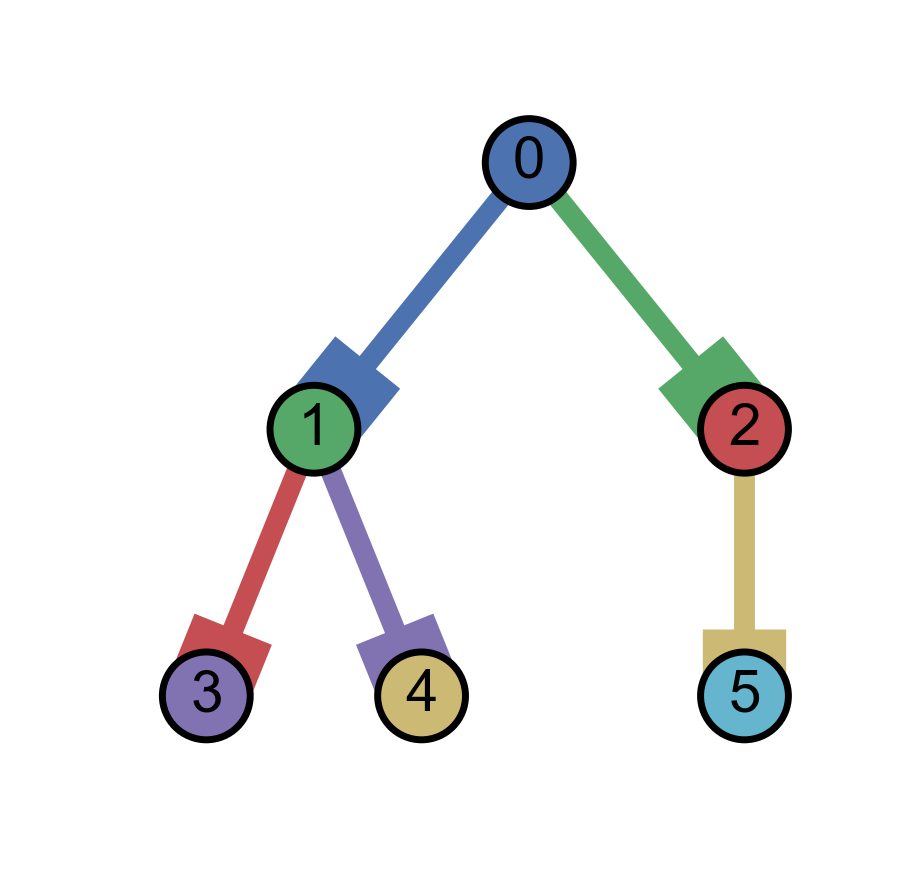
\includegraphics[width=0.4\linewidth,keepaspectratio,trim={0 2cm 0 2cm},clip]{./simulation/tree/tree_6.png}\label{fig:tree_6_graph}}\qquad
			\subfloat[][]{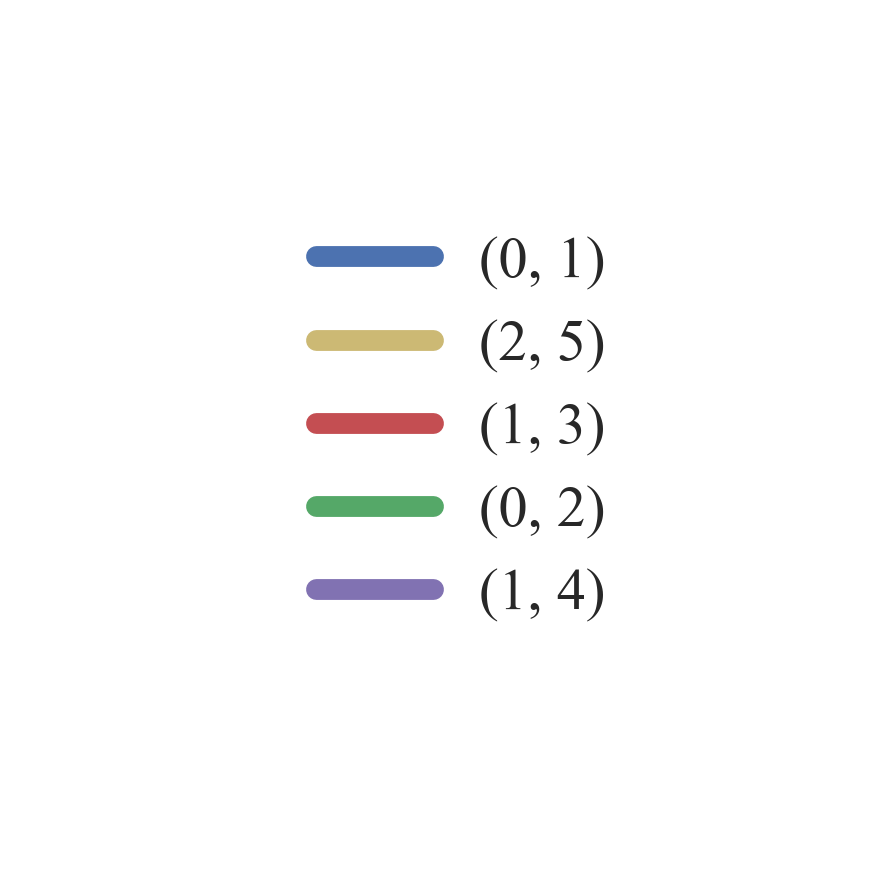
\includegraphics[width=0.4\linewidth,keepaspectratio,trim={0 2cm 0 2cm},clip]{./simulation/tree/tree_6_legend.png}\label{fig:tree_6_graph_legend}}
			\newline
			\subfloat[][]{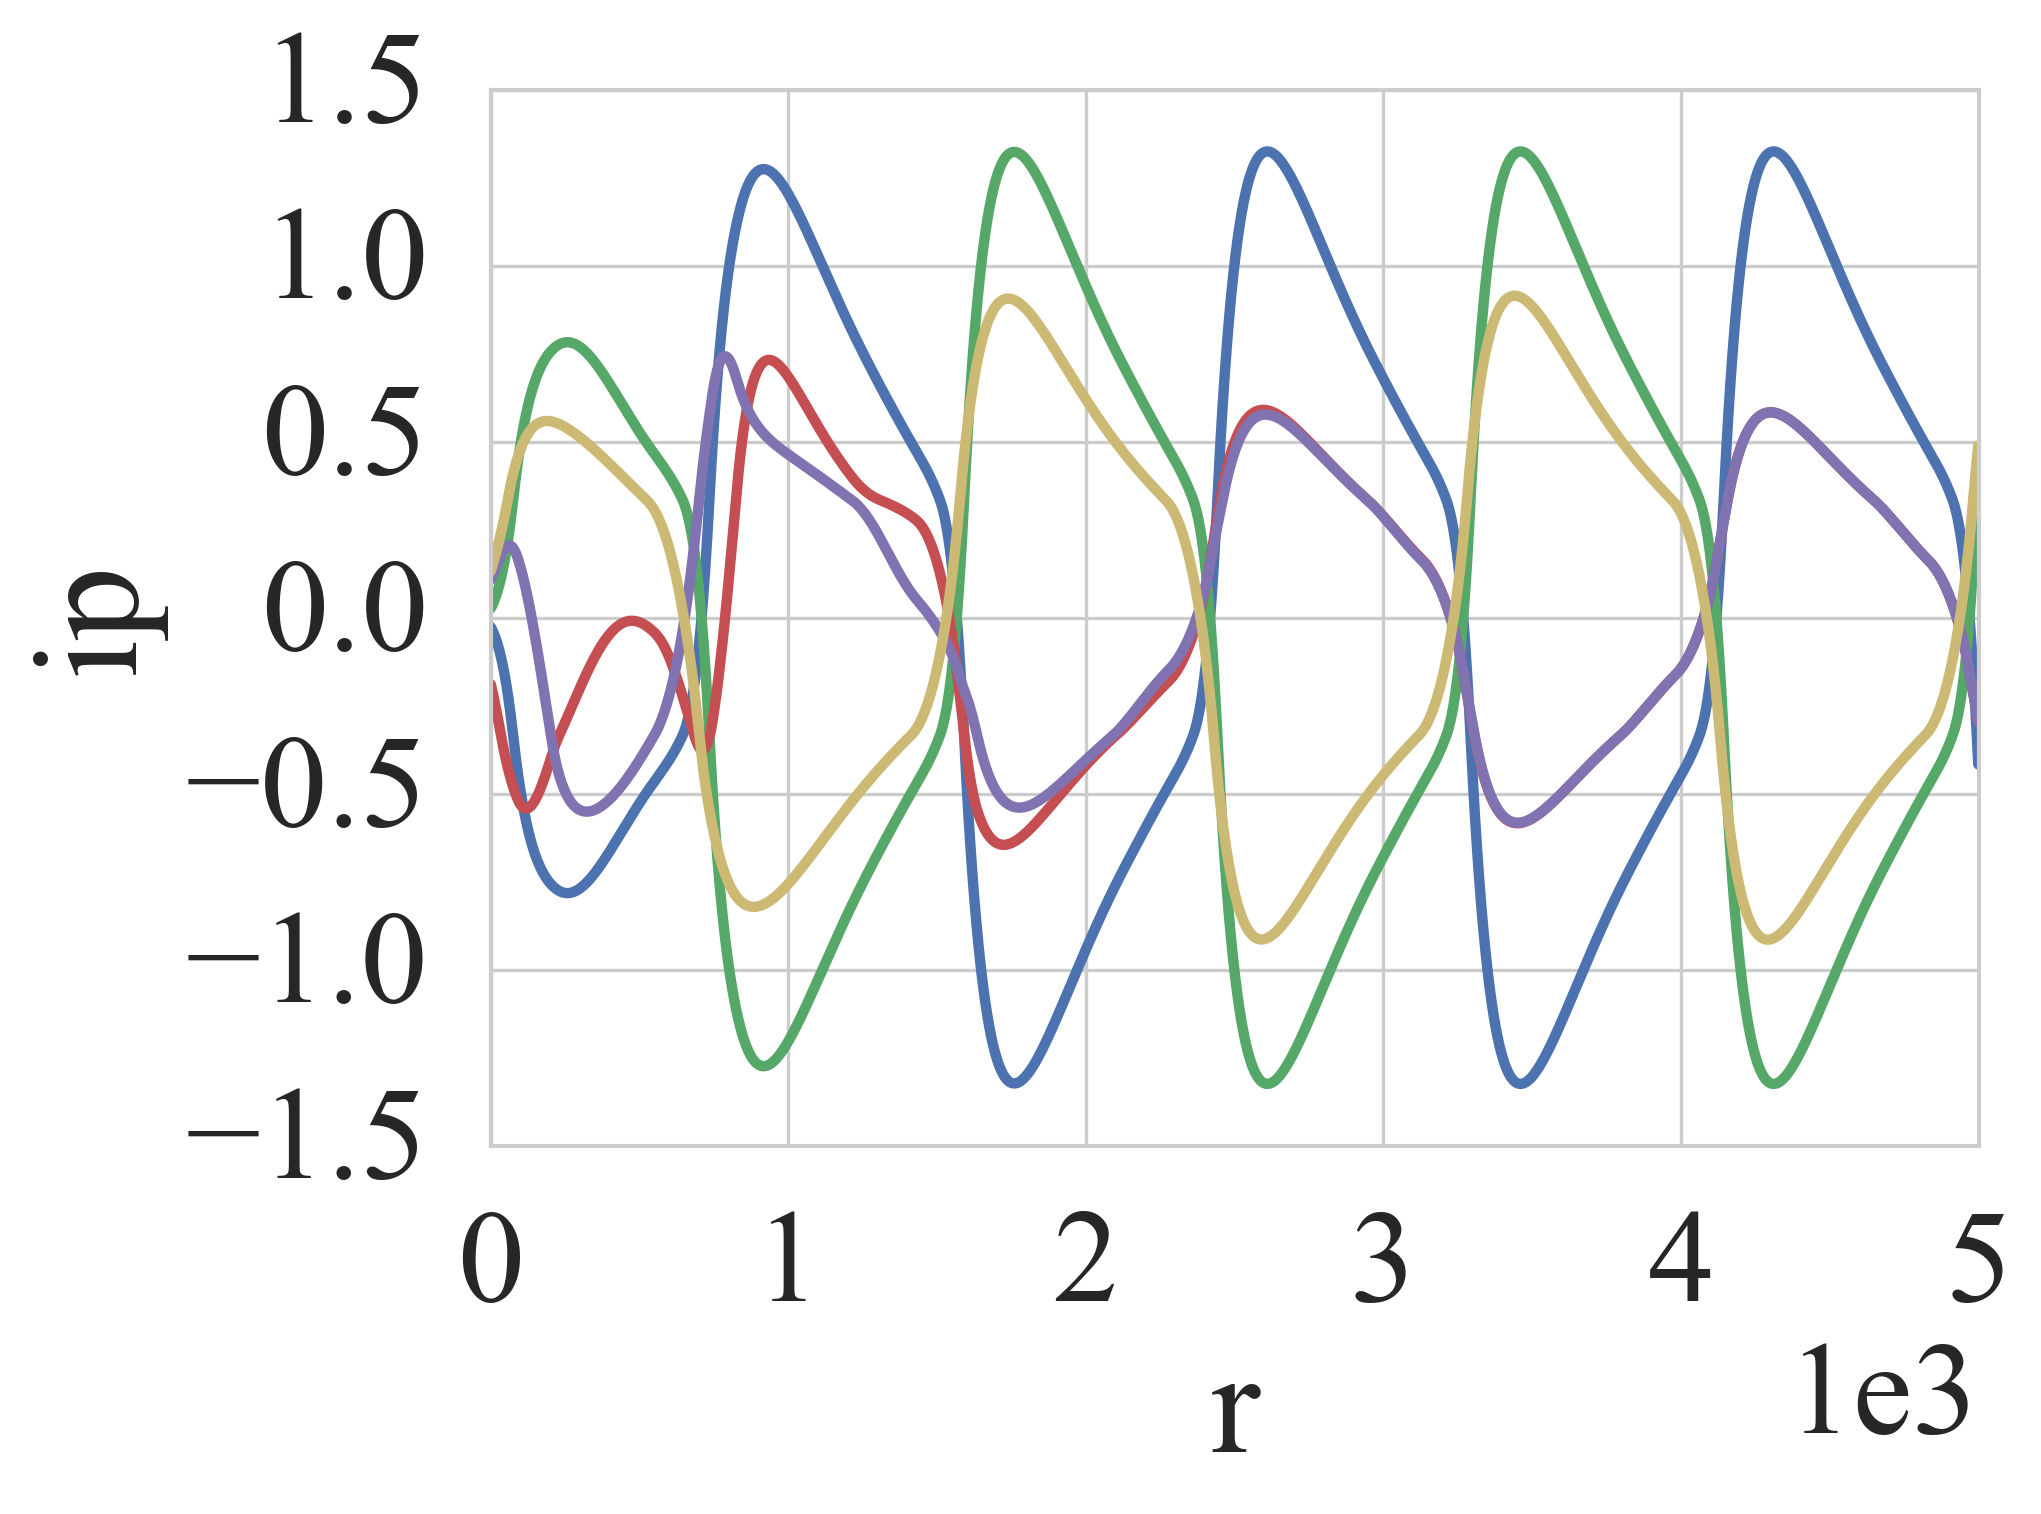
\includegraphics[width=0.4\linewidth,keepaspectratio]{./simulation/tree/tree_6_ip.png}\label{fig:tree_6_ip}}\qquad
			\subfloat[][]{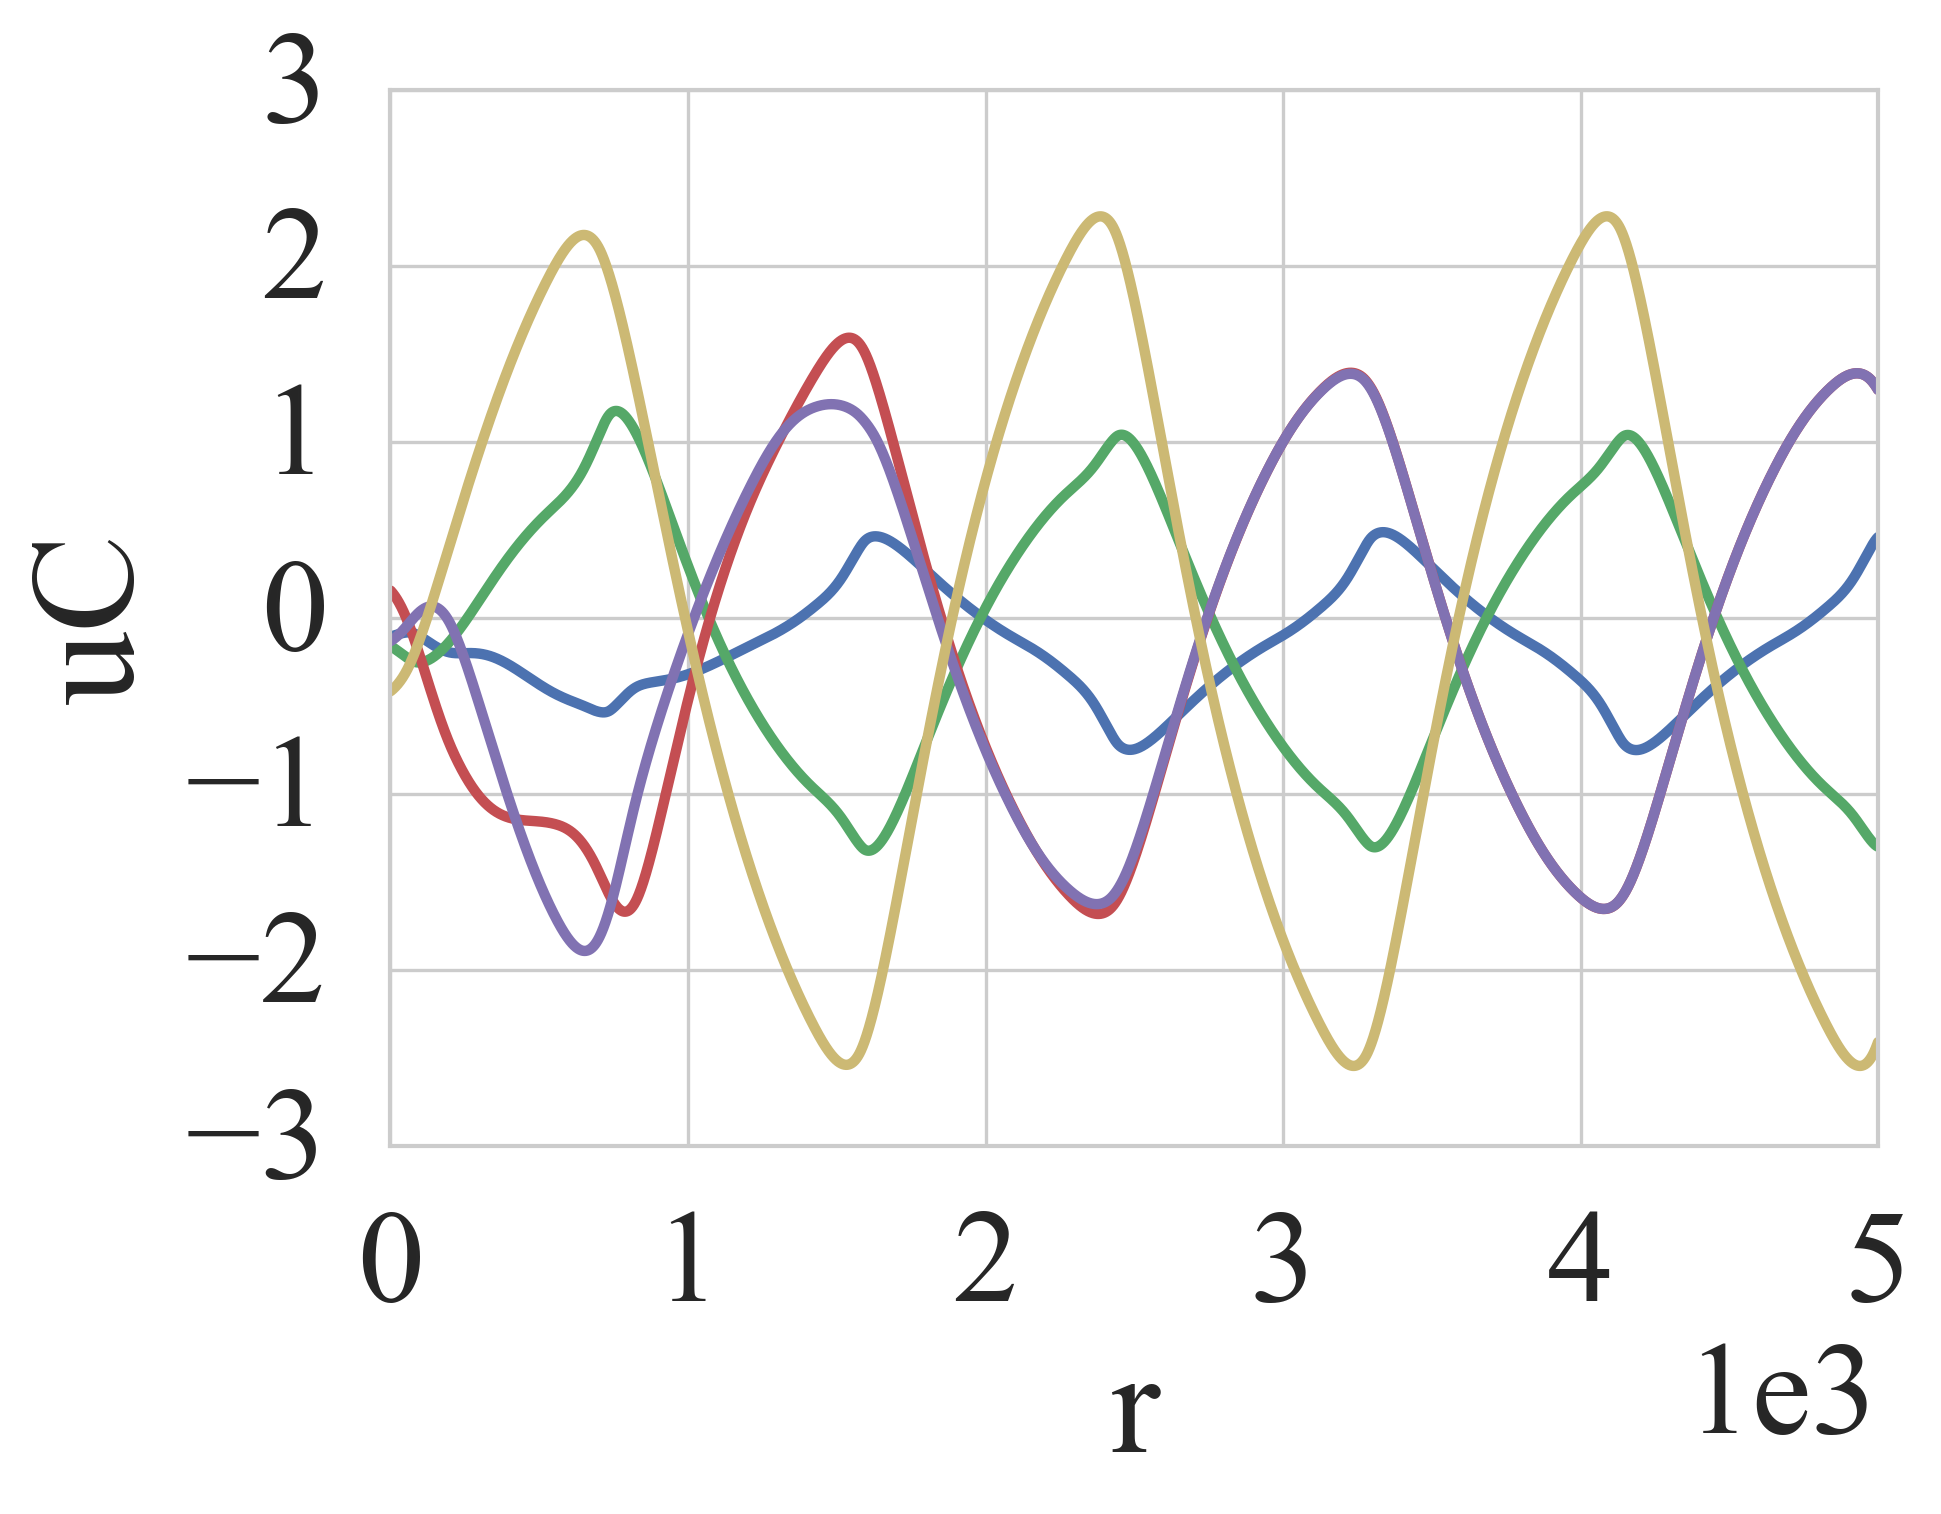
\includegraphics[width=0.4\linewidth,keepaspectratio]{./simulation/tree/tree_6_uC.png}\label{fig:tree_6_uC}}
			
					
			\caption[Tree simulations]{A simple tree of \Pes.}
			\label{fig:tree}
		\end{figure}

	\subsection{Two linked cycles of \emph{Physarum} Elements}

		Finally, we combine the features of paths and cycles to obtain a \Pns as shown in \Fref{fig:dumbbell_graph}. \Fref{fig:dumbbell_graph_legend} defines a color coding which serves as a legend for the plots of \Fref{fig:dumbbell}.

		The proposed topology is meant as an first attempt of exploring the connection between the workings of our model and the behavior of live \P. We do so by interpreting the \Pn in \Fref{fig:dumbbell_graph} as an abstract representation of the way \P was modeled as a living system of delay-coupled mechanical oscillators as mentioned in the short survey of existing modeling approaches~\cite{PhysRevLett.85.2026}. The two $3$-cycles represent the reservoirs while the path of length $1$ constitutes the channel connecting them. In the original wet-lab experiment \P showed rich self-synchronizing oscillation patterns between the distinct reservoirs with both in-phase and anti-phase entrainment. It is interesting to ask, whether our model can reproduce any of the observed effects.

		To explore the behavior of our model, we present $3$ distinct simulation instances. First we look towards the capacitor voltages to find symmetric oscillations in perfect anti-phase within the two $3-cycles$. After a brief period of entrainment, the edges in the two cycles converge symmetrically around the value the channel edges $(0,5)$ converges to, see \Fref{fig:dumbbell_3_1_uC_symmetric_positive}, \Fref{fig:dumbbell_uC_symmetric_negative} and \Fref{fig:dumbbell_uC_asymmetric}. The picture is similar to what was observed for the diamond graph, except that the non-bridge edges, \ie the cycle edges, can now sustain oscillation. While this anti-phase entrainment is reminiscent of the behavior delay-coupled oscillators, we were not able to get our model to show in-phase entrainment. In fact, given the invariants we were able to proof, it is unlikely to be possible.

		With regards to the currents flowing in the \Pn, we observe scenarios that are intuitive. The currents in both cycles can be identical and flowing in the same direction, either clockwise, see \Fref{fig:dumbbell_ip_symmetric_negative}, or counter-clockwise, see \Fref{fig:dumbbell_3_1_ip_symmetric_positive}. Furthermore, the currents can flow in the opposite directions adding two more scenarios. \Fref{fig:dumbbell_ip_asymmetric} shows one of them with the l.h.s $3$-cycle showing counter-clockwise flow while the r.h.s $3$-cycle exhibits clockwise flow. A scenario where currents are damped is not shown. In contrast to isolated $3$-cycles, the coupling between the two cycles induces oscillations in the circular flows.	Interesting in all scenarios is the behavior of the channel edge $(0,5)$ which shows periodic flow reversals with a period of $T \approx 1629 $ rounds and large peak flows. Again $100$ repetitions of the simulation suggests the period to be independent on the initial conditions within the range we tested.

		Clearly, the model we propose yields only a crude approximation of the behavior of \P. Based on the high degree of abstraction and the relatively simple model, it is surprising that effects like flow reversal and anti-phase entrainment emerge naturally. It is also apparent, that we are limited to simple topologies of \Pes if we are to make sense of the behavior analytically. Of course this does not prohibit using the model as a black box for more complicated and/or larger graphs.


		\begin{figure}
			\centering
			\subfloat[][]{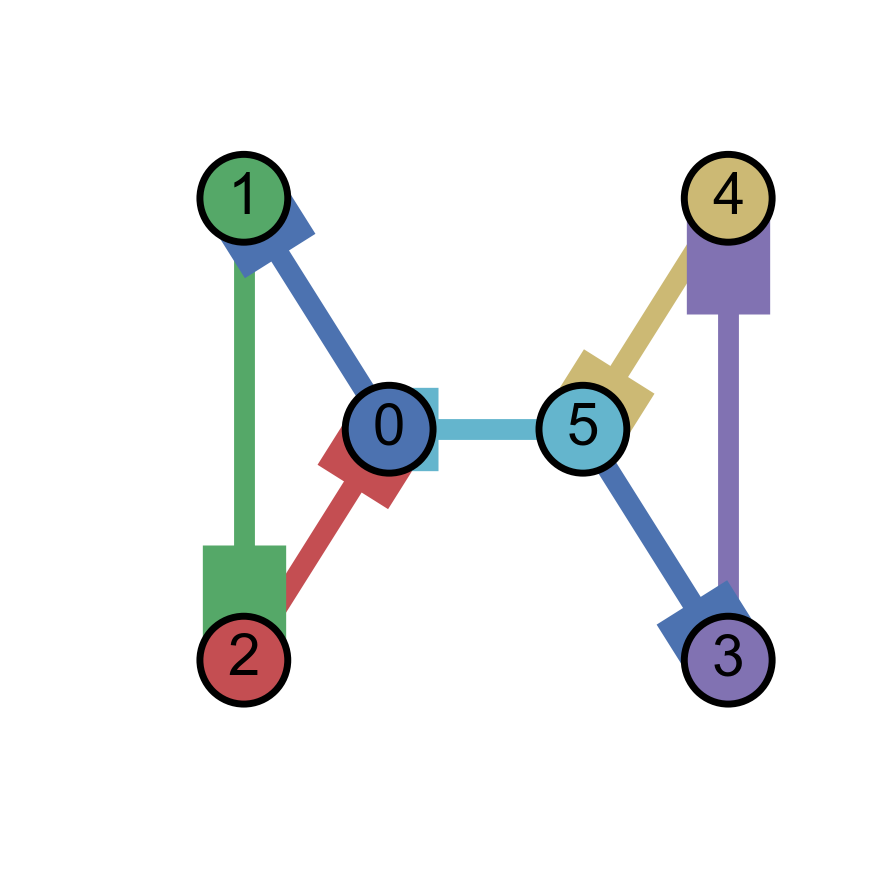
\includegraphics[width=0.35\linewidth,keepaspectratio,trim={0 4cm 0 3cm},clip]{./simulation/dumbbell/dumbbell_3_1.png}\label{fig:dumbbell_graph}}\qquad
			\subfloat[][]{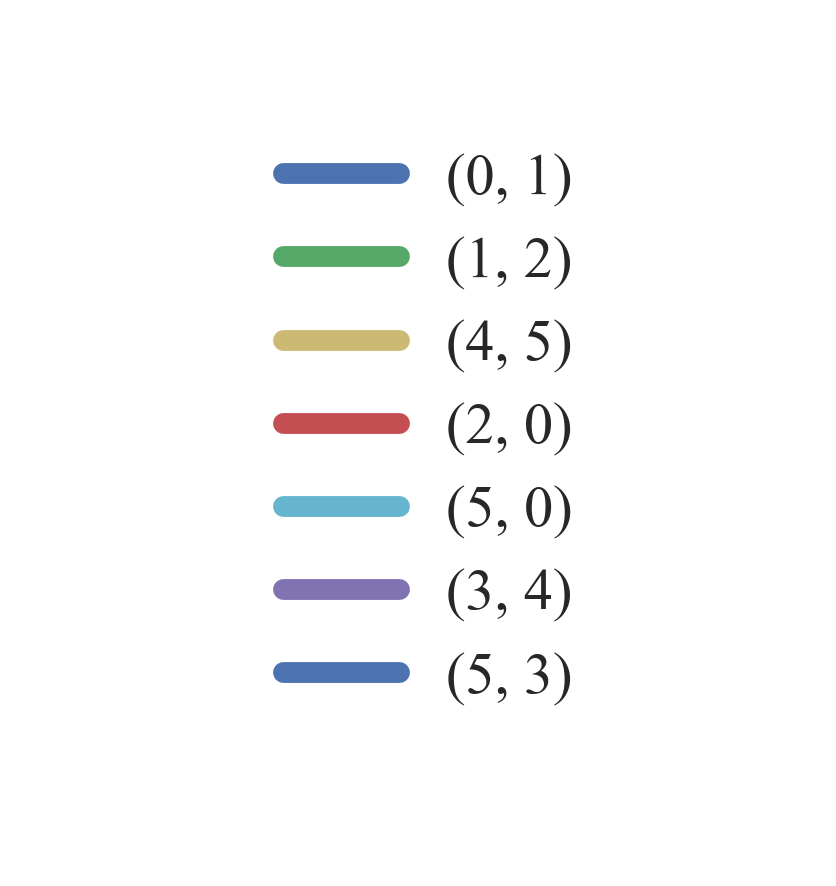
\includegraphics[width=0.35\linewidth,keepaspectratio,trim={0 4cm 0 3cm},clip]{./simulation/dumbbell/dumbbell_3_1_legend.png}\label{fig:dumbbell_graph_legend}}
			\newline
			\subfloat[][]{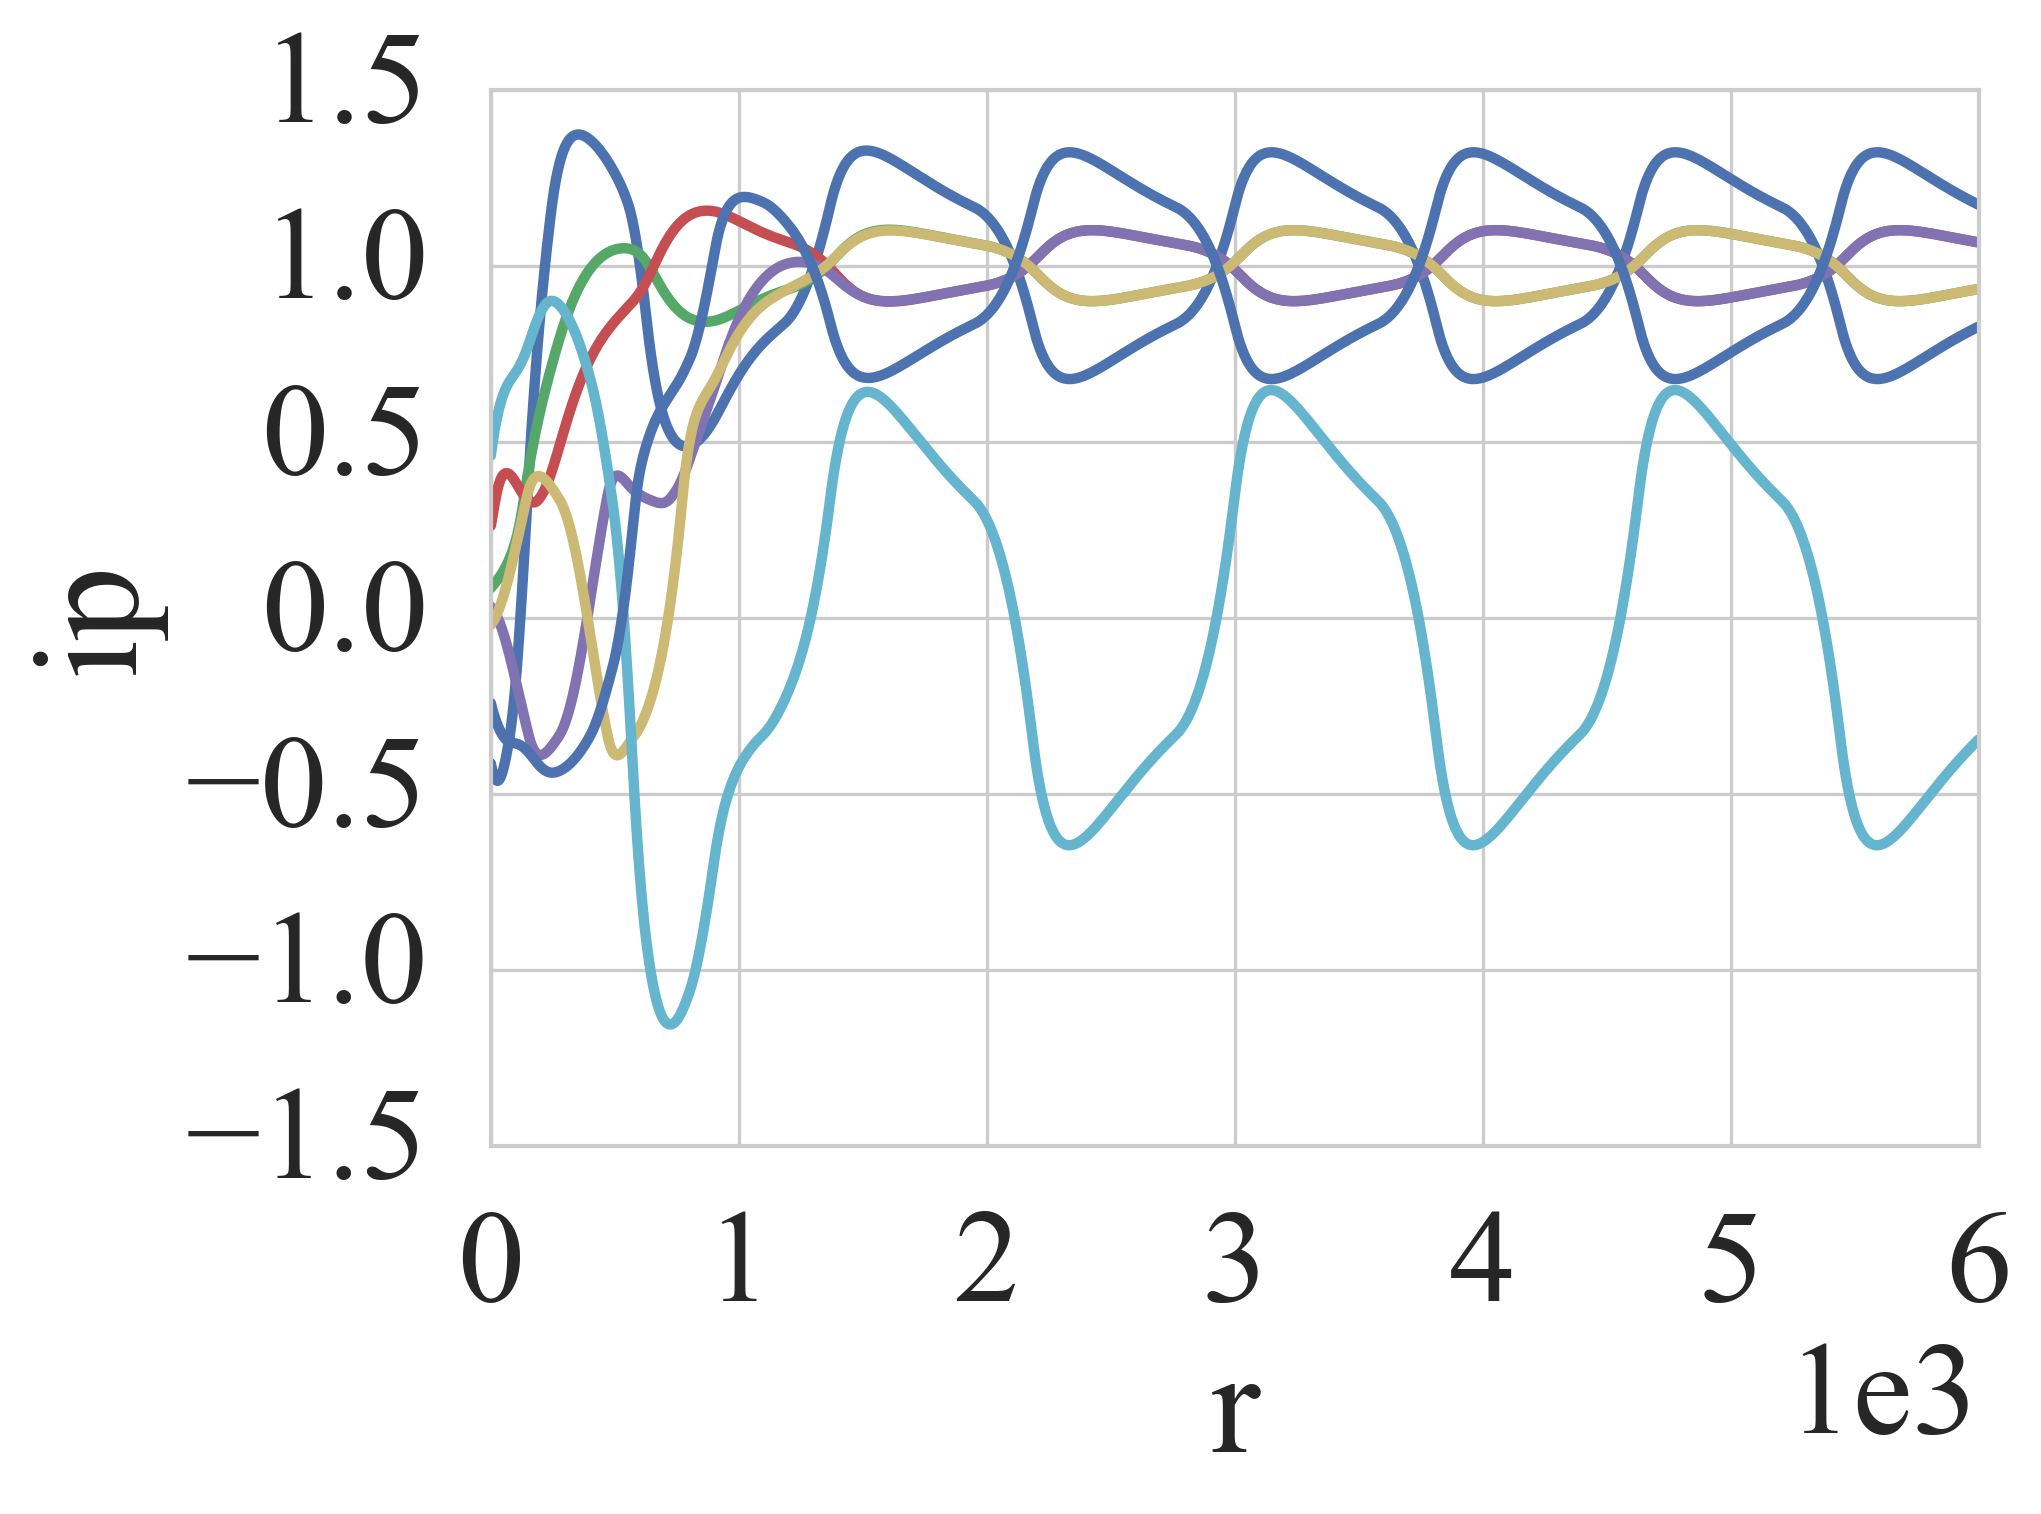
\includegraphics[width=0.4\linewidth,keepaspectratio]{./simulation/dumbbell/dumbbell_3_1_ip_symmetric_positive.png}\label{fig:dumbbell_3_1_ip_symmetric_positive}}\qquad
			\subfloat[][]{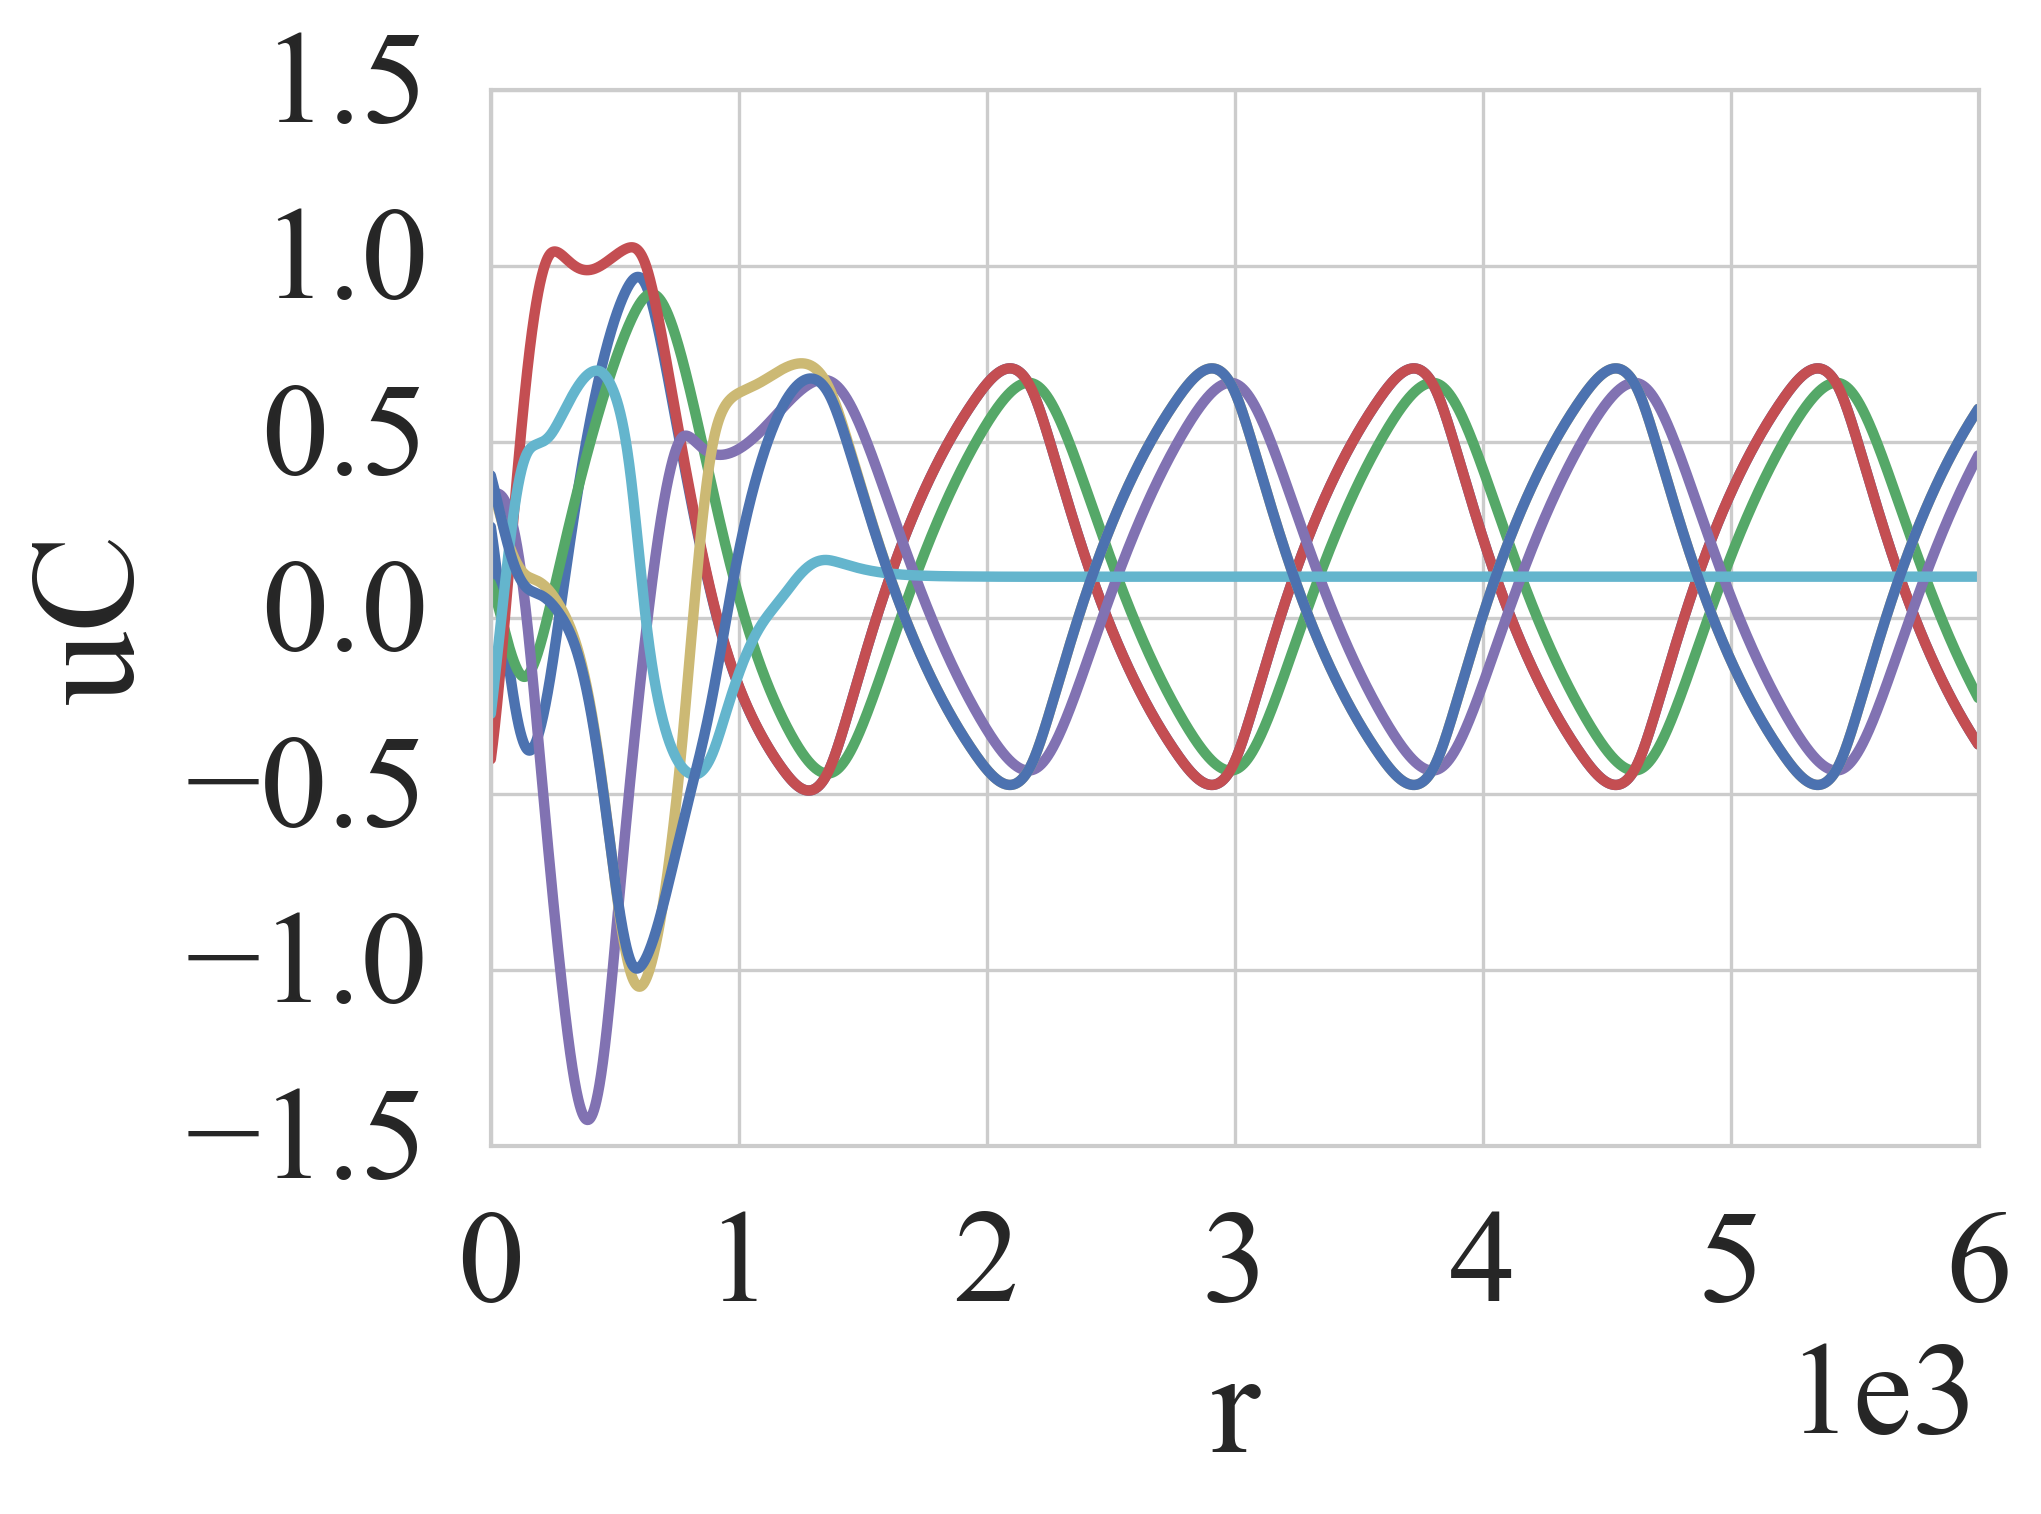
\includegraphics[width=0.4\linewidth,keepaspectratio]{./simulation/dumbbell/dumbbell_3_1_uC_symmetric_positive.png}\label{fig:dumbbell_3_1_uC_symmetric_positive}}
			\newline
			\subfloat[][]{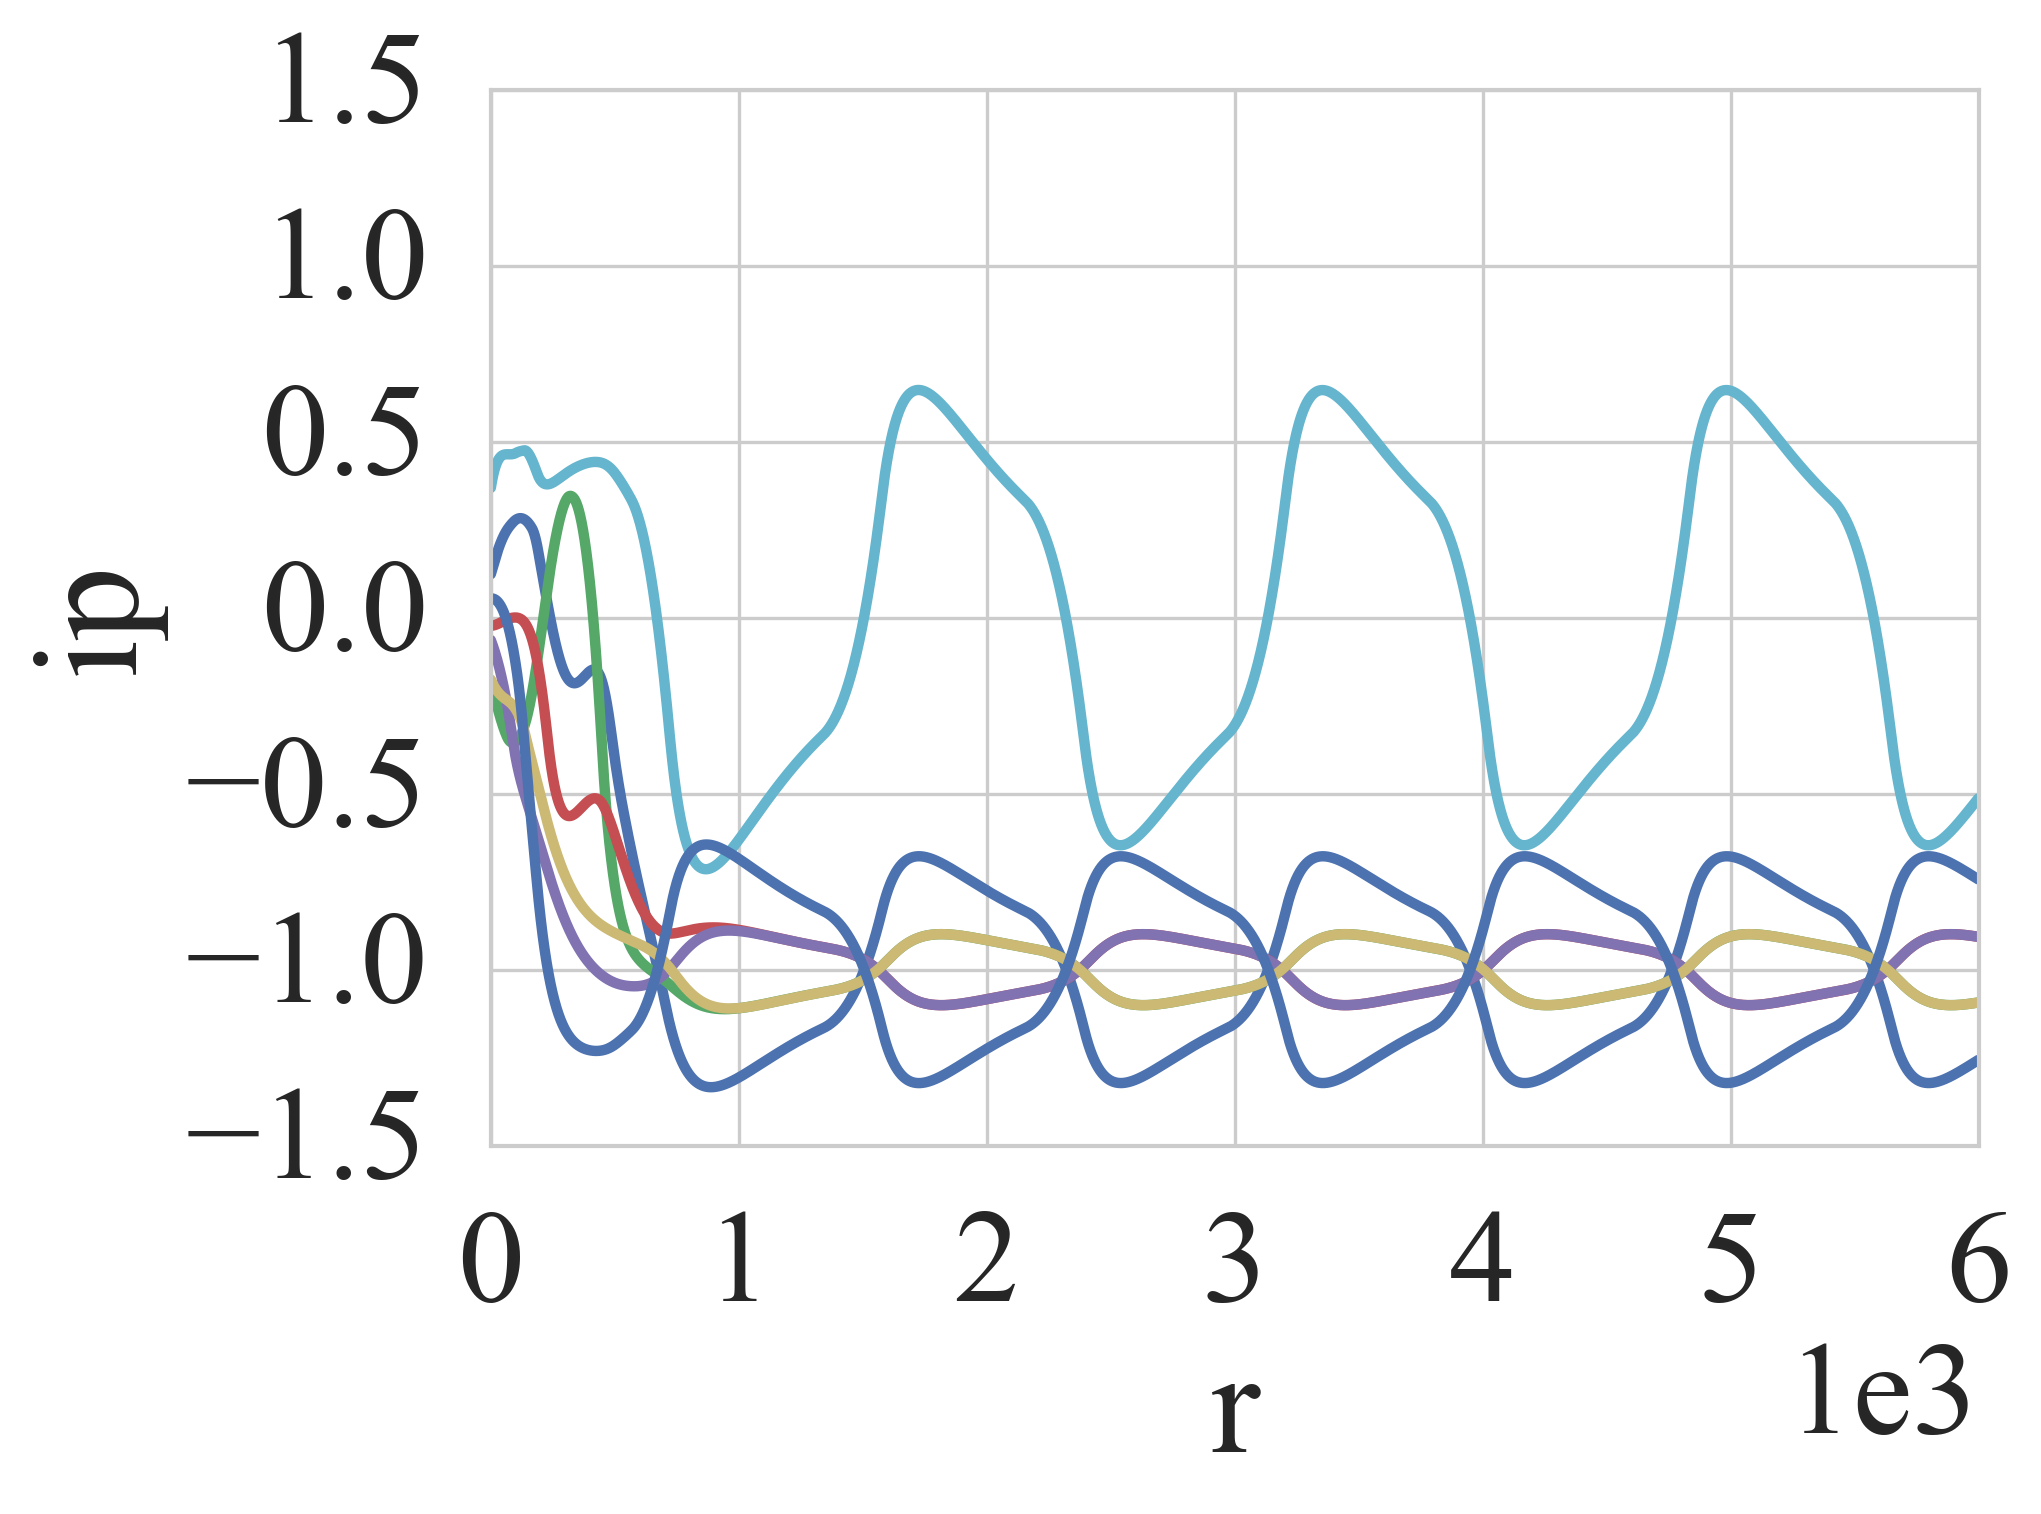
\includegraphics[width=0.4\linewidth,keepaspectratio]{./simulation/dumbbell/dumbbell_3_1_ip_symmetric_negative.png}\label{fig:dumbbell_ip_symmetric_negative}}\qquad
			\subfloat[][]{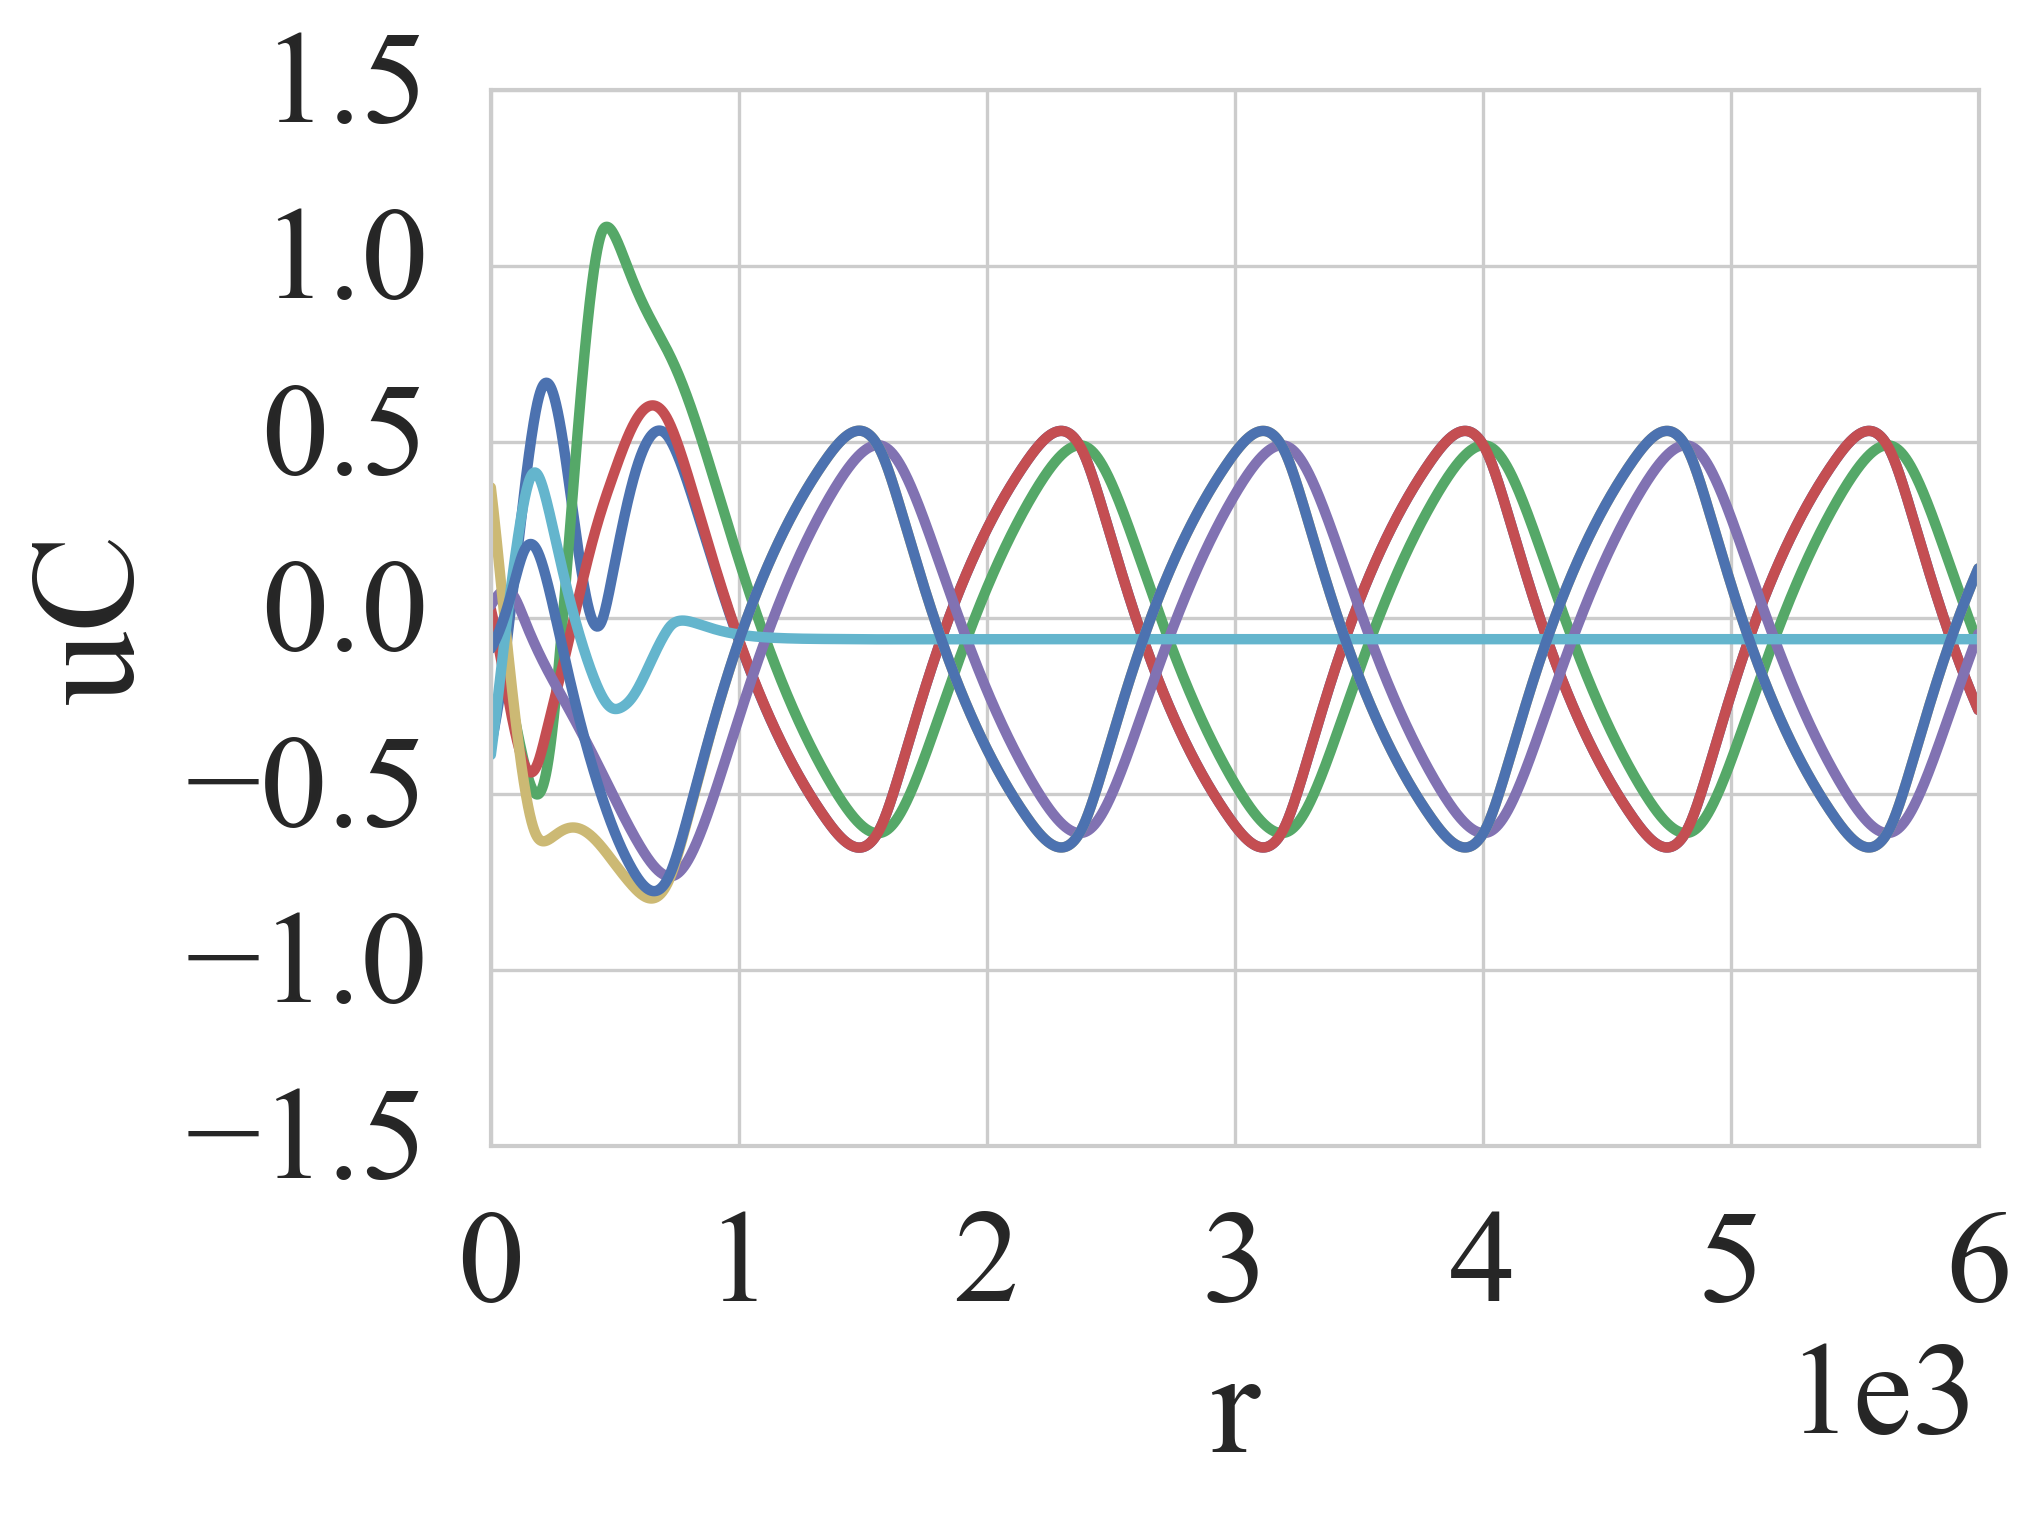
\includegraphics[width=0.4\linewidth,keepaspectratio]{./simulation/dumbbell/dumbbell_3_1_uC_symmetric_negative.png}\label{fig:dumbbell_uC_symmetric_negative}}
			\newline
			\subfloat[][]{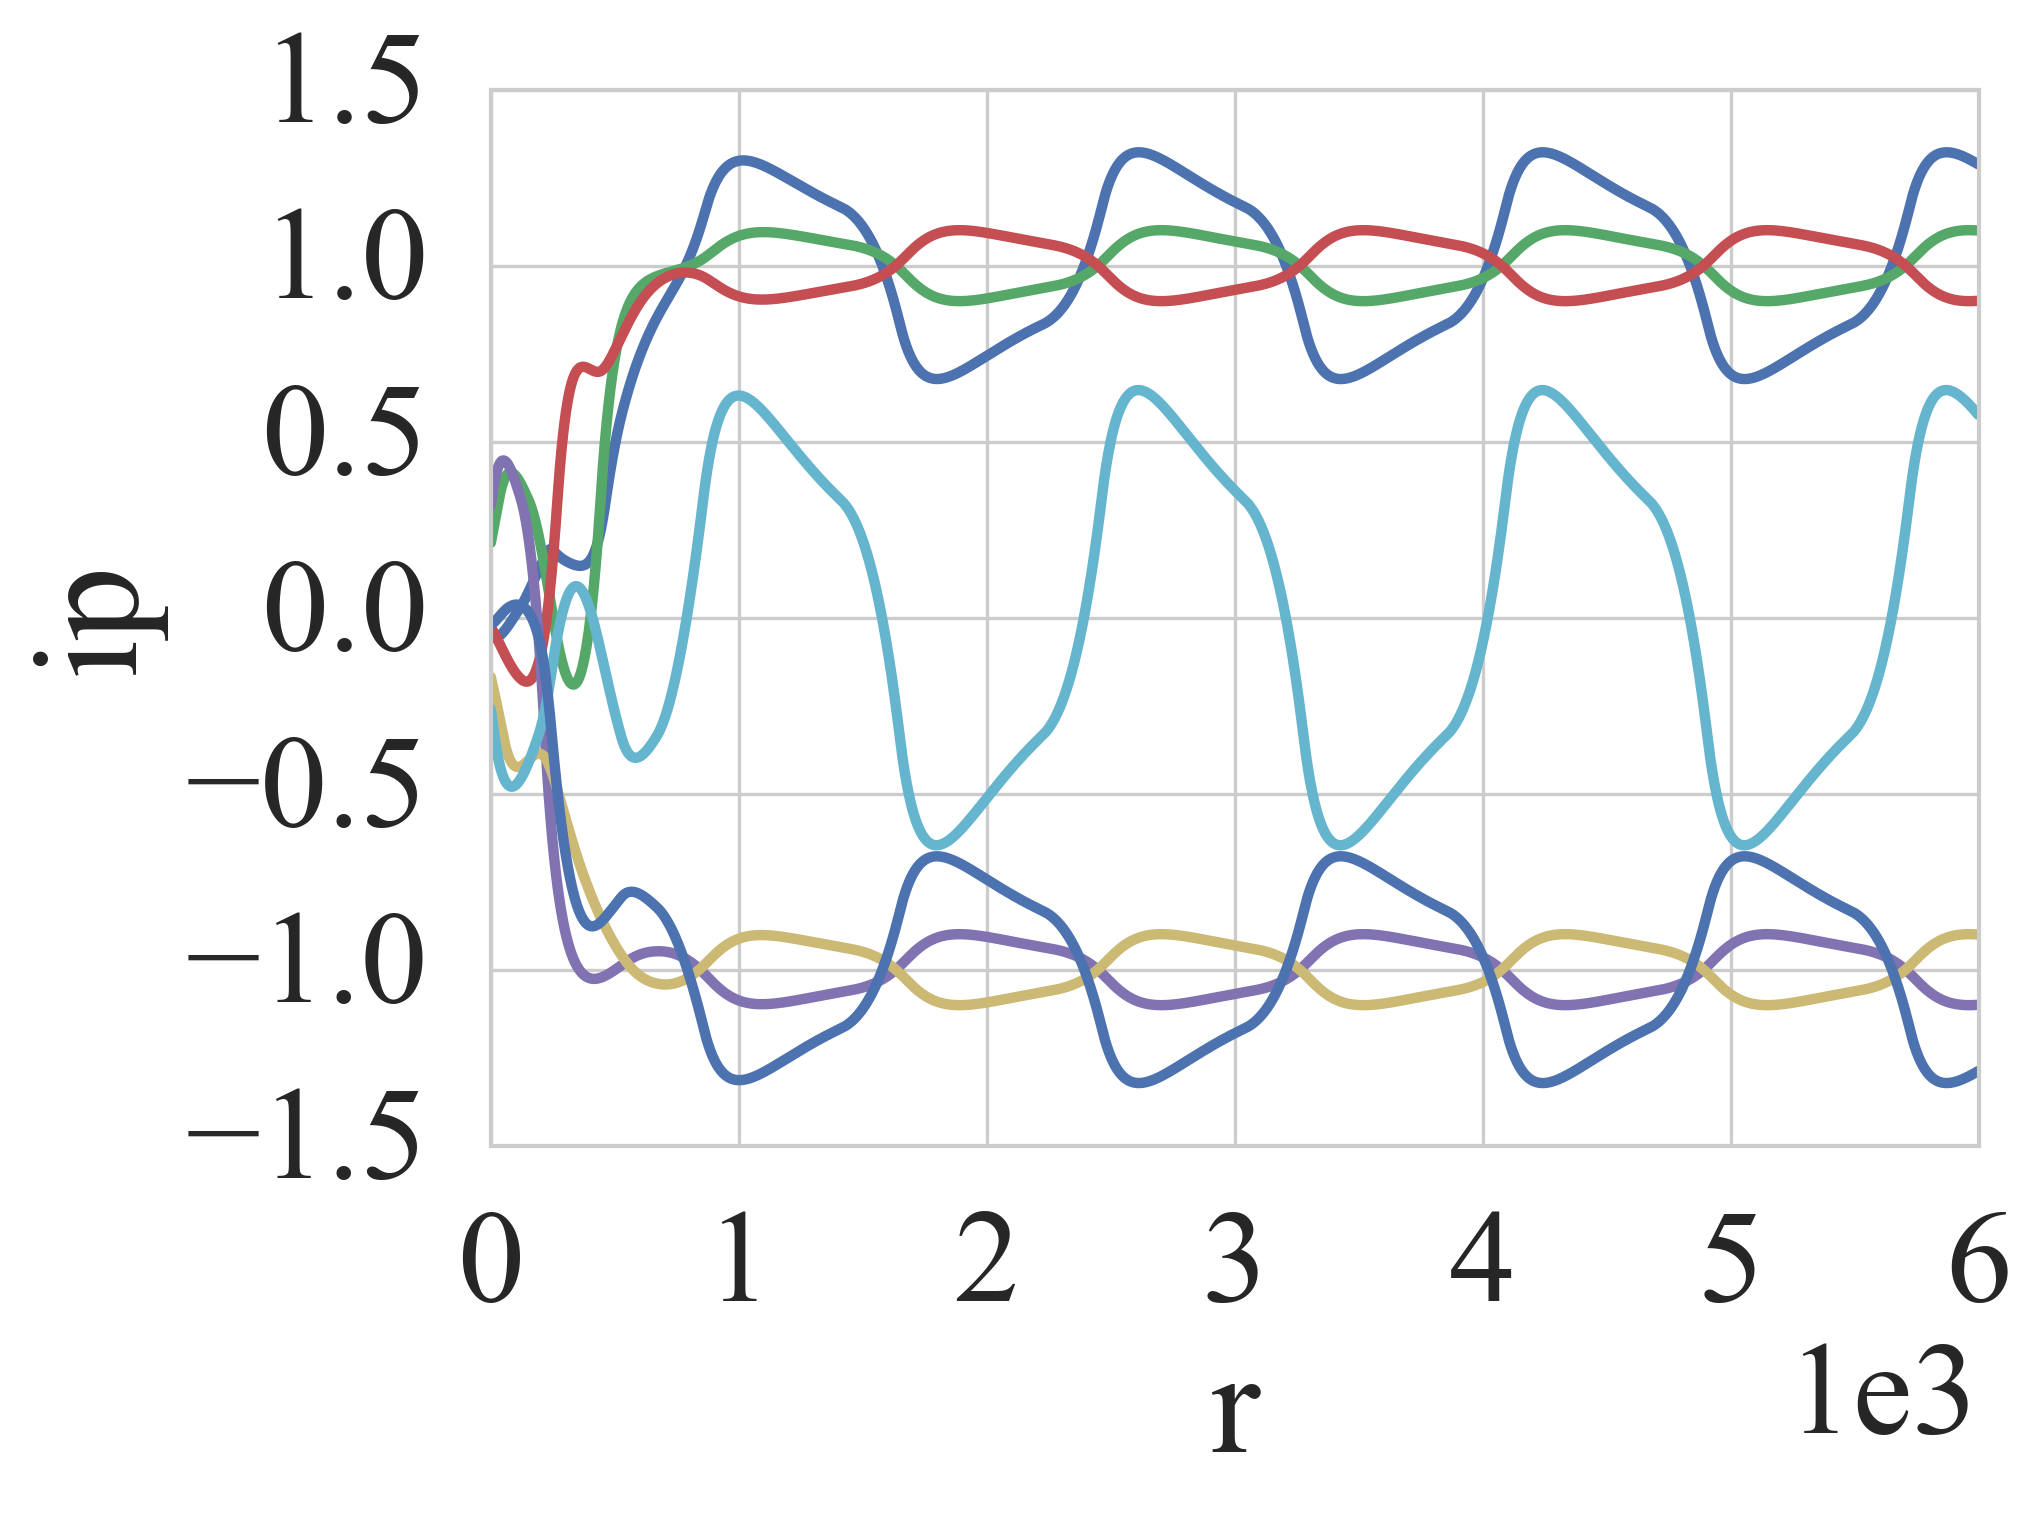
\includegraphics[width=0.4\linewidth,keepaspectratio]{./simulation/dumbbell/dumbbell_3_1_ip_asymmetric.png}\label{fig:dumbbell_ip_asymmetric}}\qquad
			\subfloat[][]{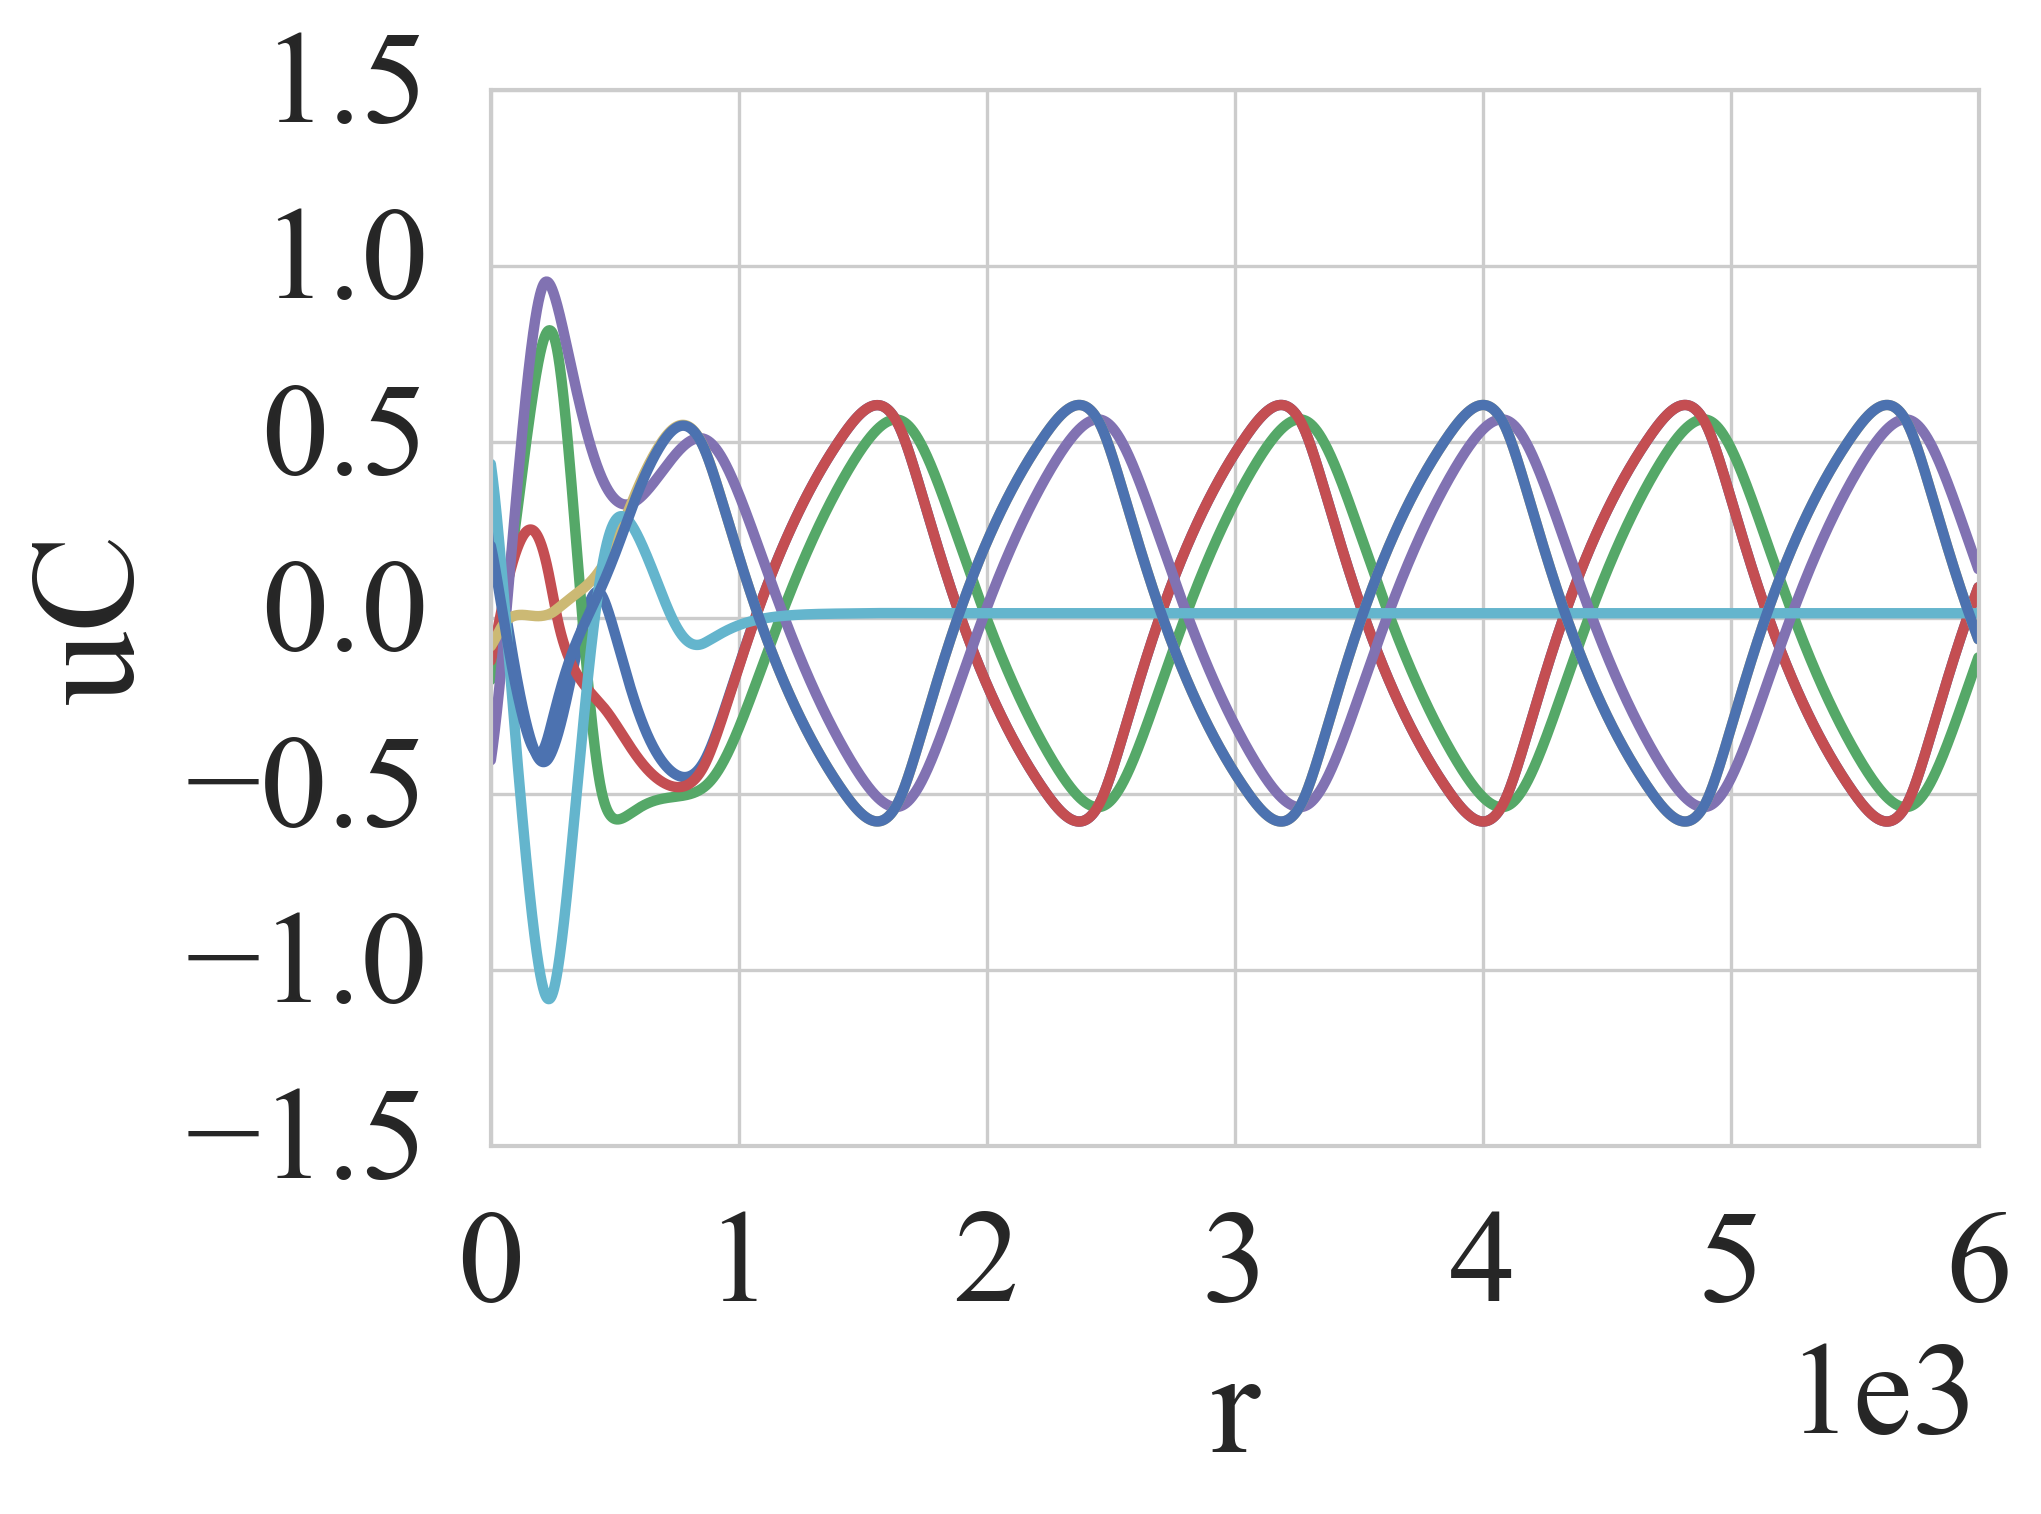
\includegraphics[width=0.4\linewidth,keepaspectratio]{./simulation/dumbbell/dumbbell_3_1_uC_asymmetric.png}\label{fig:dumbbell_uC_asymmetric}}
			
			\caption[Path simulations]{A \Pn designed to mimic aspects of the delay-coupled oscillator model of \P.}
			\label{fig:dumbbell}
		\end{figure}

	\subsection{\emph{Physarum} Elements and Changing Topology}

		Finally, we show that the model is capable of adapting to changes in the topology of the underlying \Pn. This is not surprising given that at the heart of our model are electronic circuits. It is possible that a formal proof of this property can be obtained.

		Here we present numerical evidence based on modifying the graph presented in the previous section, see \Fref{fig:dumbbell_graph}. Needless to say, \Fref{fig:dumbbell_graph_legend} defines a color coding which serves as a legend for the plots of \Fref{fig:robustness}.

		In \Fref{fig:dumbbell_ip_changing} and \Fref{fig:ddumbbell_uC_changing} the channel edge $(5,0)$ was removed from the \Pn at point $r=4000$ and reinserted at $r=8000$. The plots illustrate how oscillations cease immediately at $r = 4000$ in favor of steady flow of opposite sign through the two cycles. The same speedy adaptation is seen in reverse when the channel edge returns at $r= 8000$.

		The procedure of changes is more complicated in  \Fref{fig:dumbbell_ip_changing_2} and \Fref{fig:dumbbell_uC_changing_2}. Here we start the simulation with the channel edge $(5,0)$ as well as one edge from the right cycle $(2,0)$ removed. As expected the plots show both the behavior of a path of length $2$ as well as constant flow in the remaining cycle. At $r = 4000$ we bring back the channel edge. At this point the \Pn consists of a $3$-cycle with a path of length $3$ attached to it. Note the complex signal shown by the circuit. The influence of the path is clearly visible, inducing oscillations in the cycle. At $r=8000$ we bring back the remaining edge and observe how the system jumps back to the expected initial behavior.


		\begin{figure}
			\centering
			
			\subfloat[][]{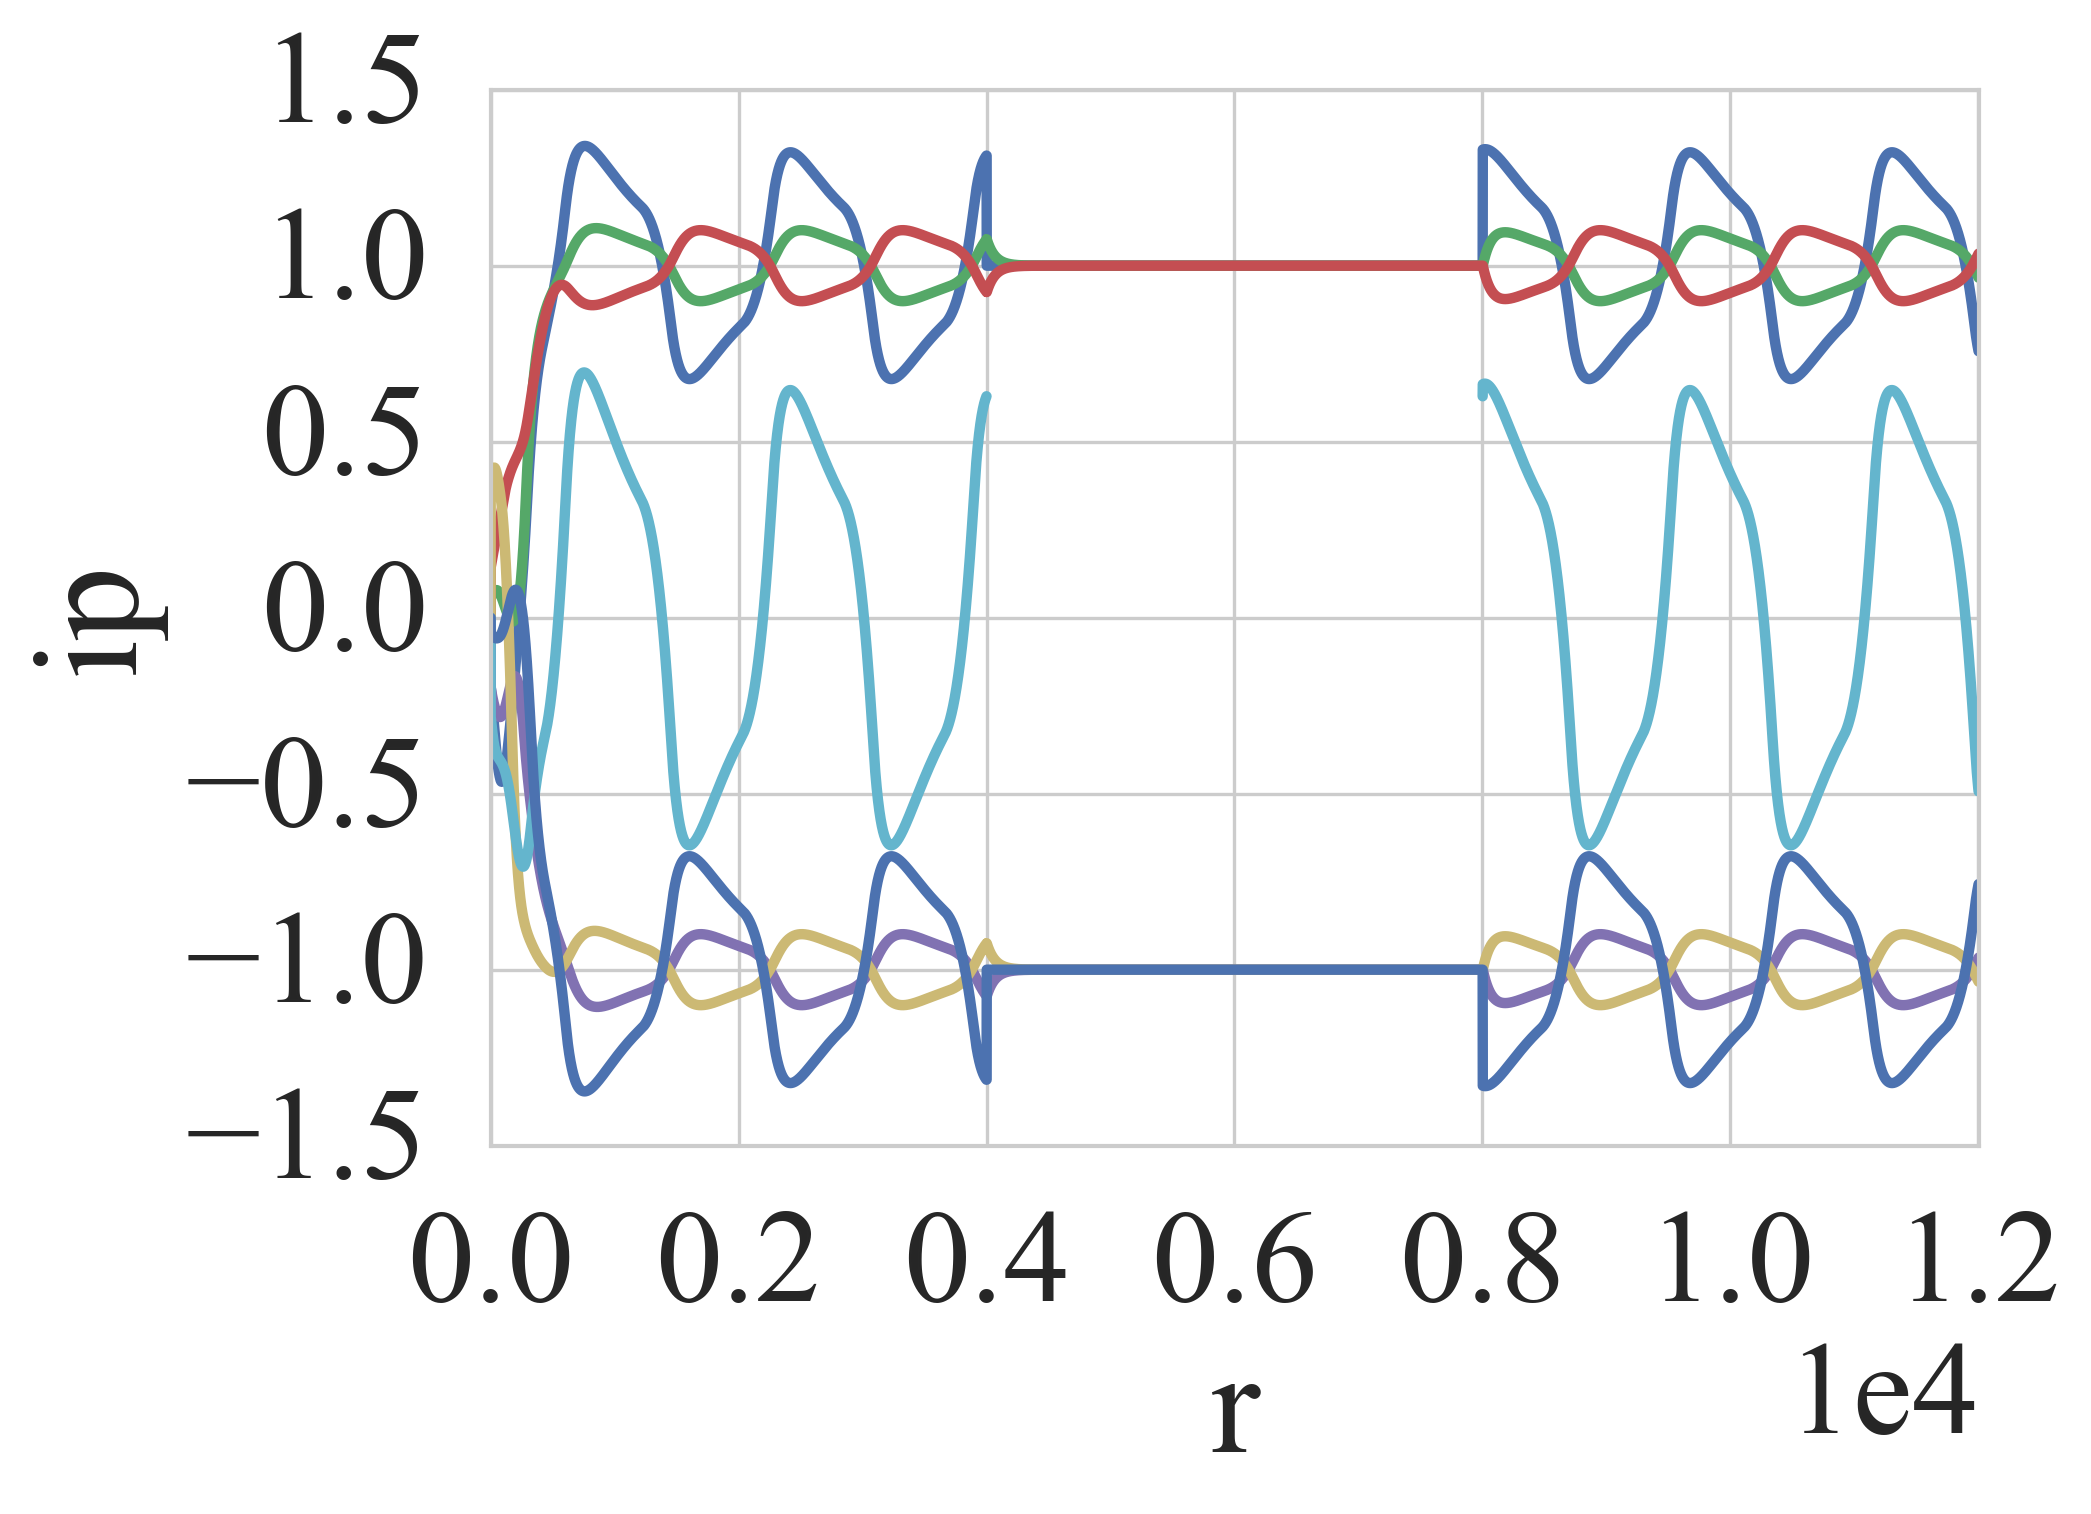
\includegraphics[width=0.4\linewidth,keepaspectratio]{./simulation/dumbbell/dumbbell_ip_changing.png}\label{fig:dumbbell_ip_changing}}\qquad
			\subfloat[][]{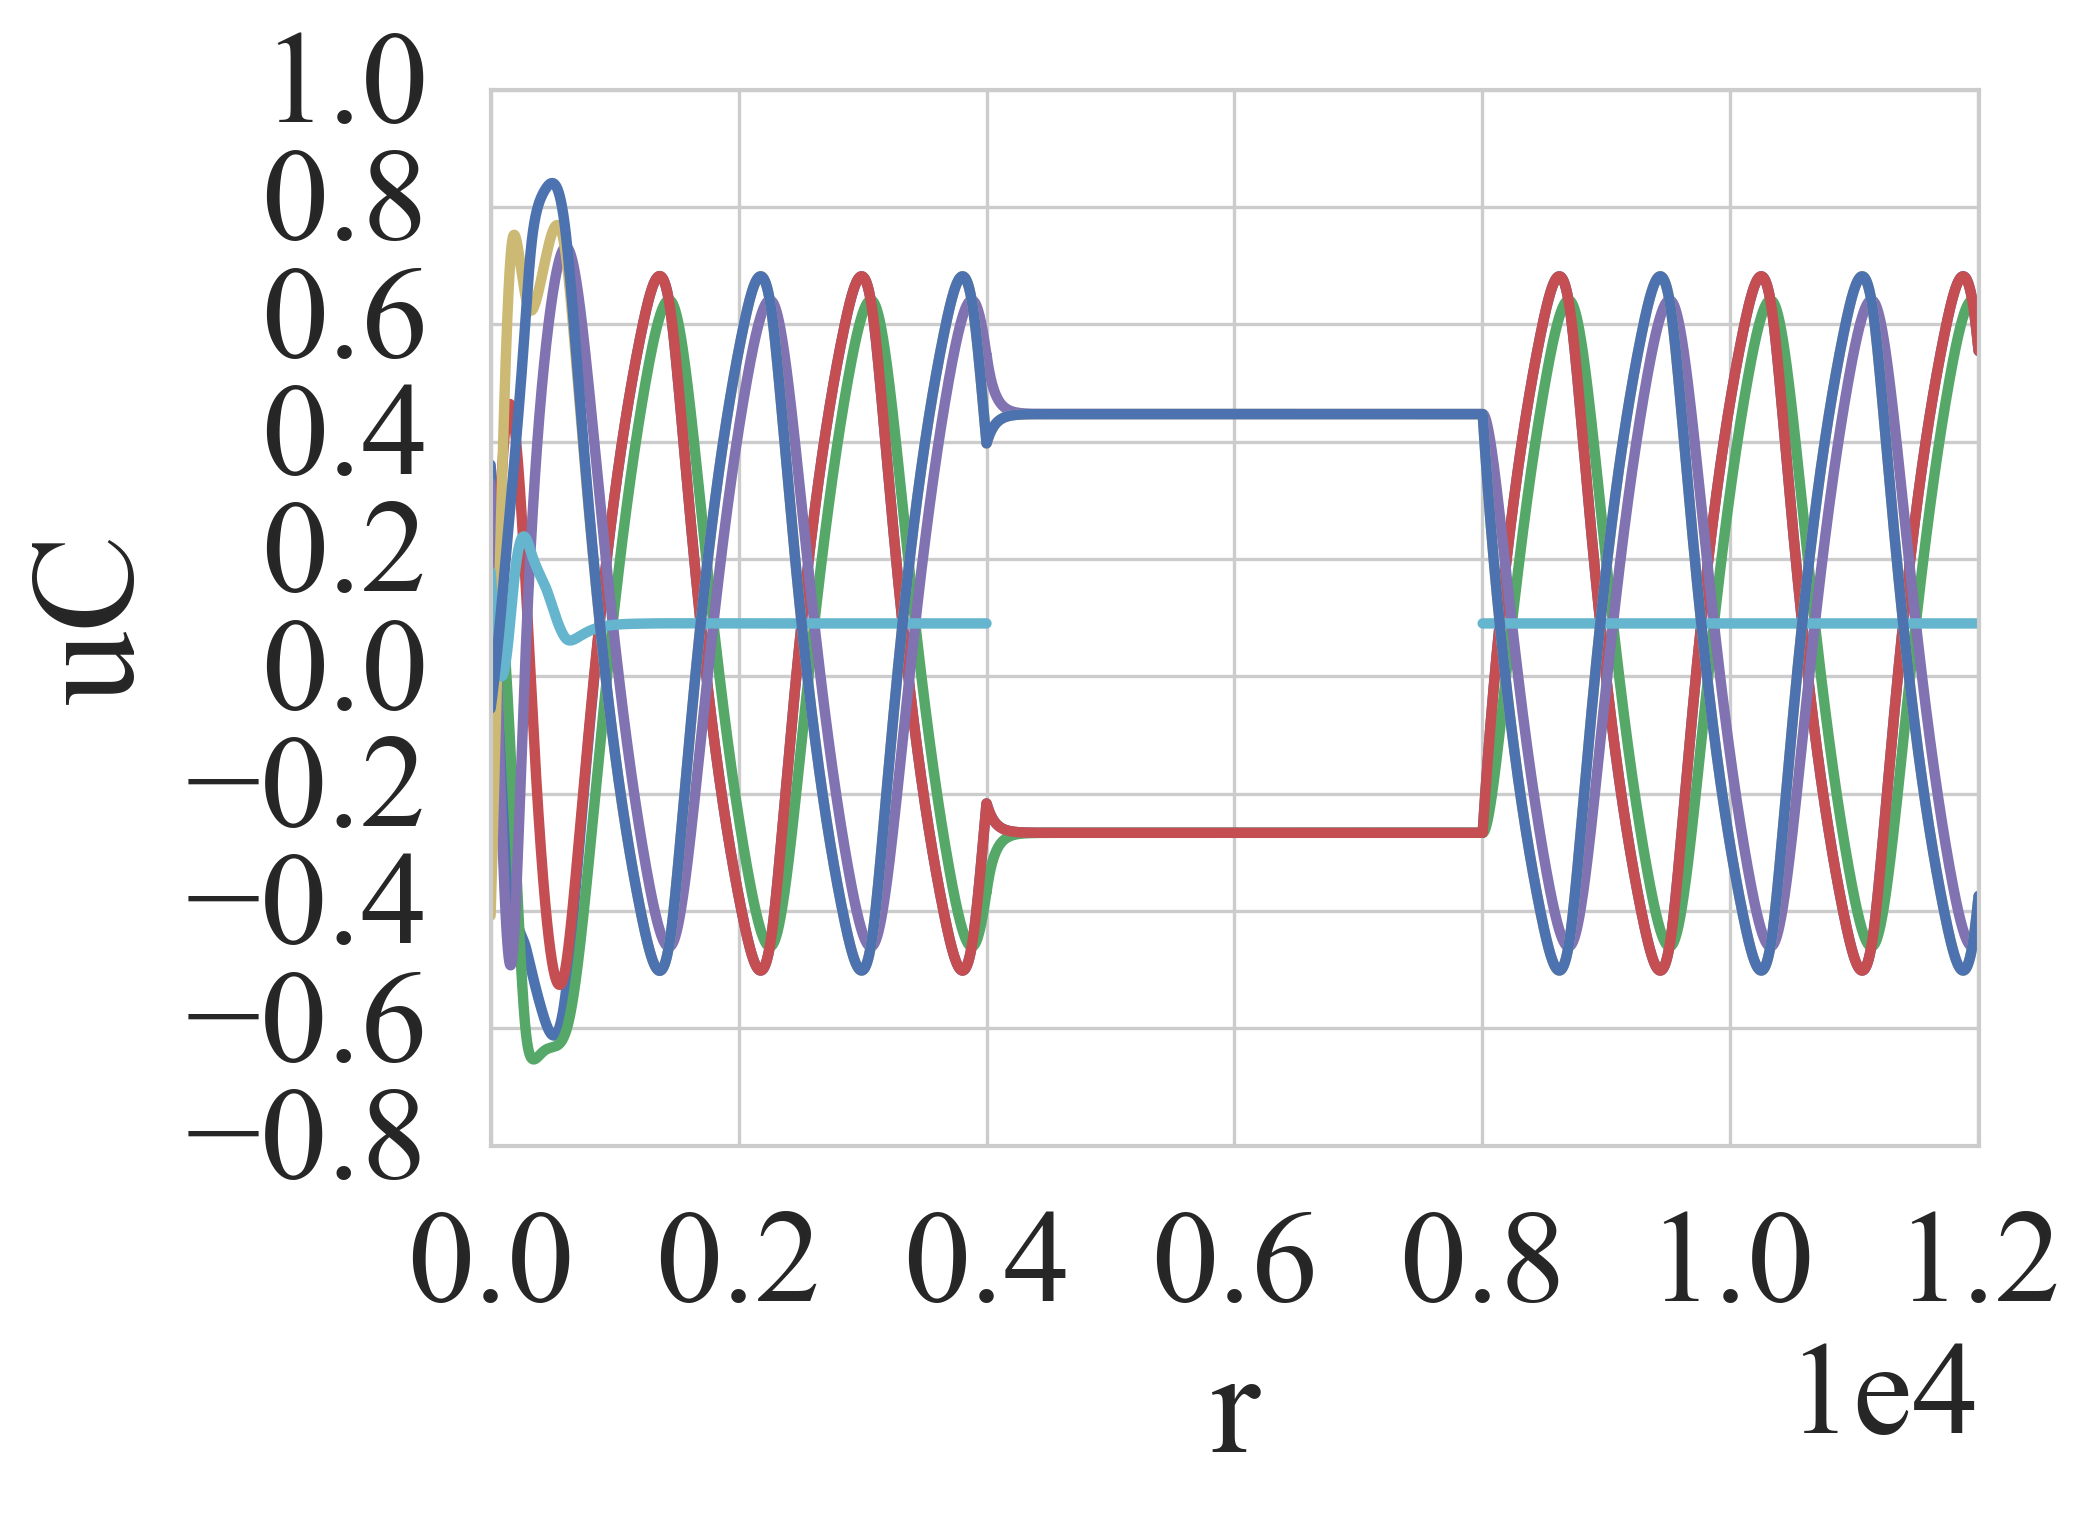
\includegraphics[width=0.4\linewidth,keepaspectratio]{./simulation/dumbbell/dumbbell_uC_changing.png}\label{fig:ddumbbell_uC_changing}}
			\newline
			\subfloat[][]{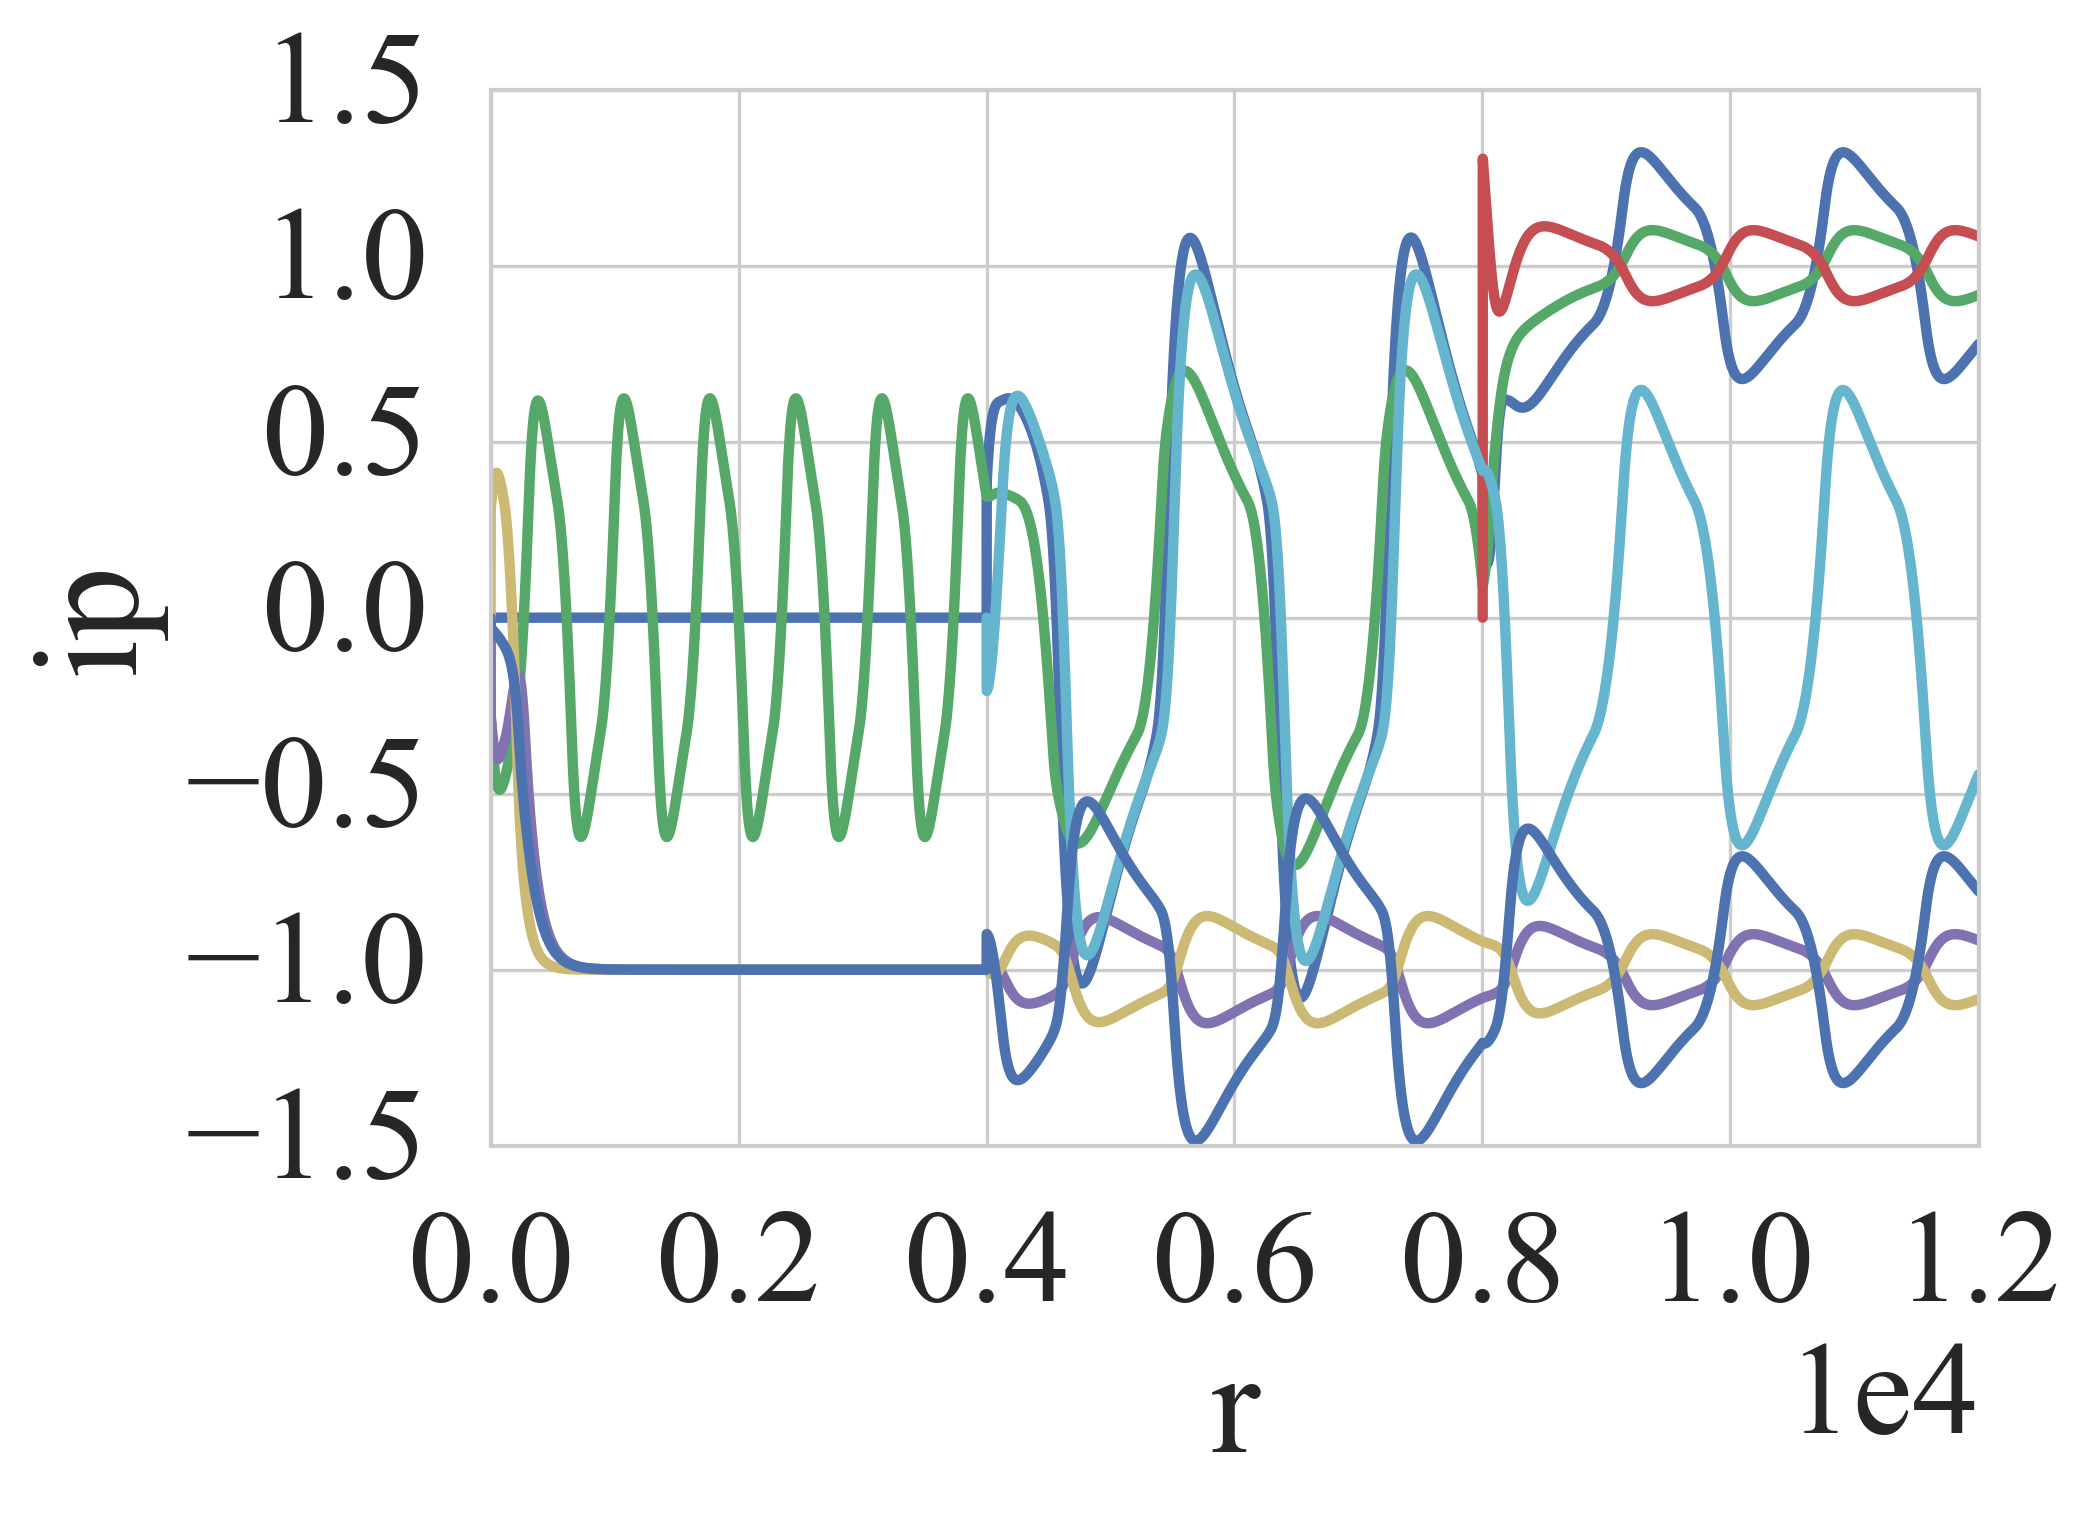
\includegraphics[width=0.4\linewidth,keepaspectratio]{./simulation/dumbbell/dumbbell_ip_changing_2.png}\label{fig:dumbbell_ip_changing_2}}\qquad
			\subfloat[][]{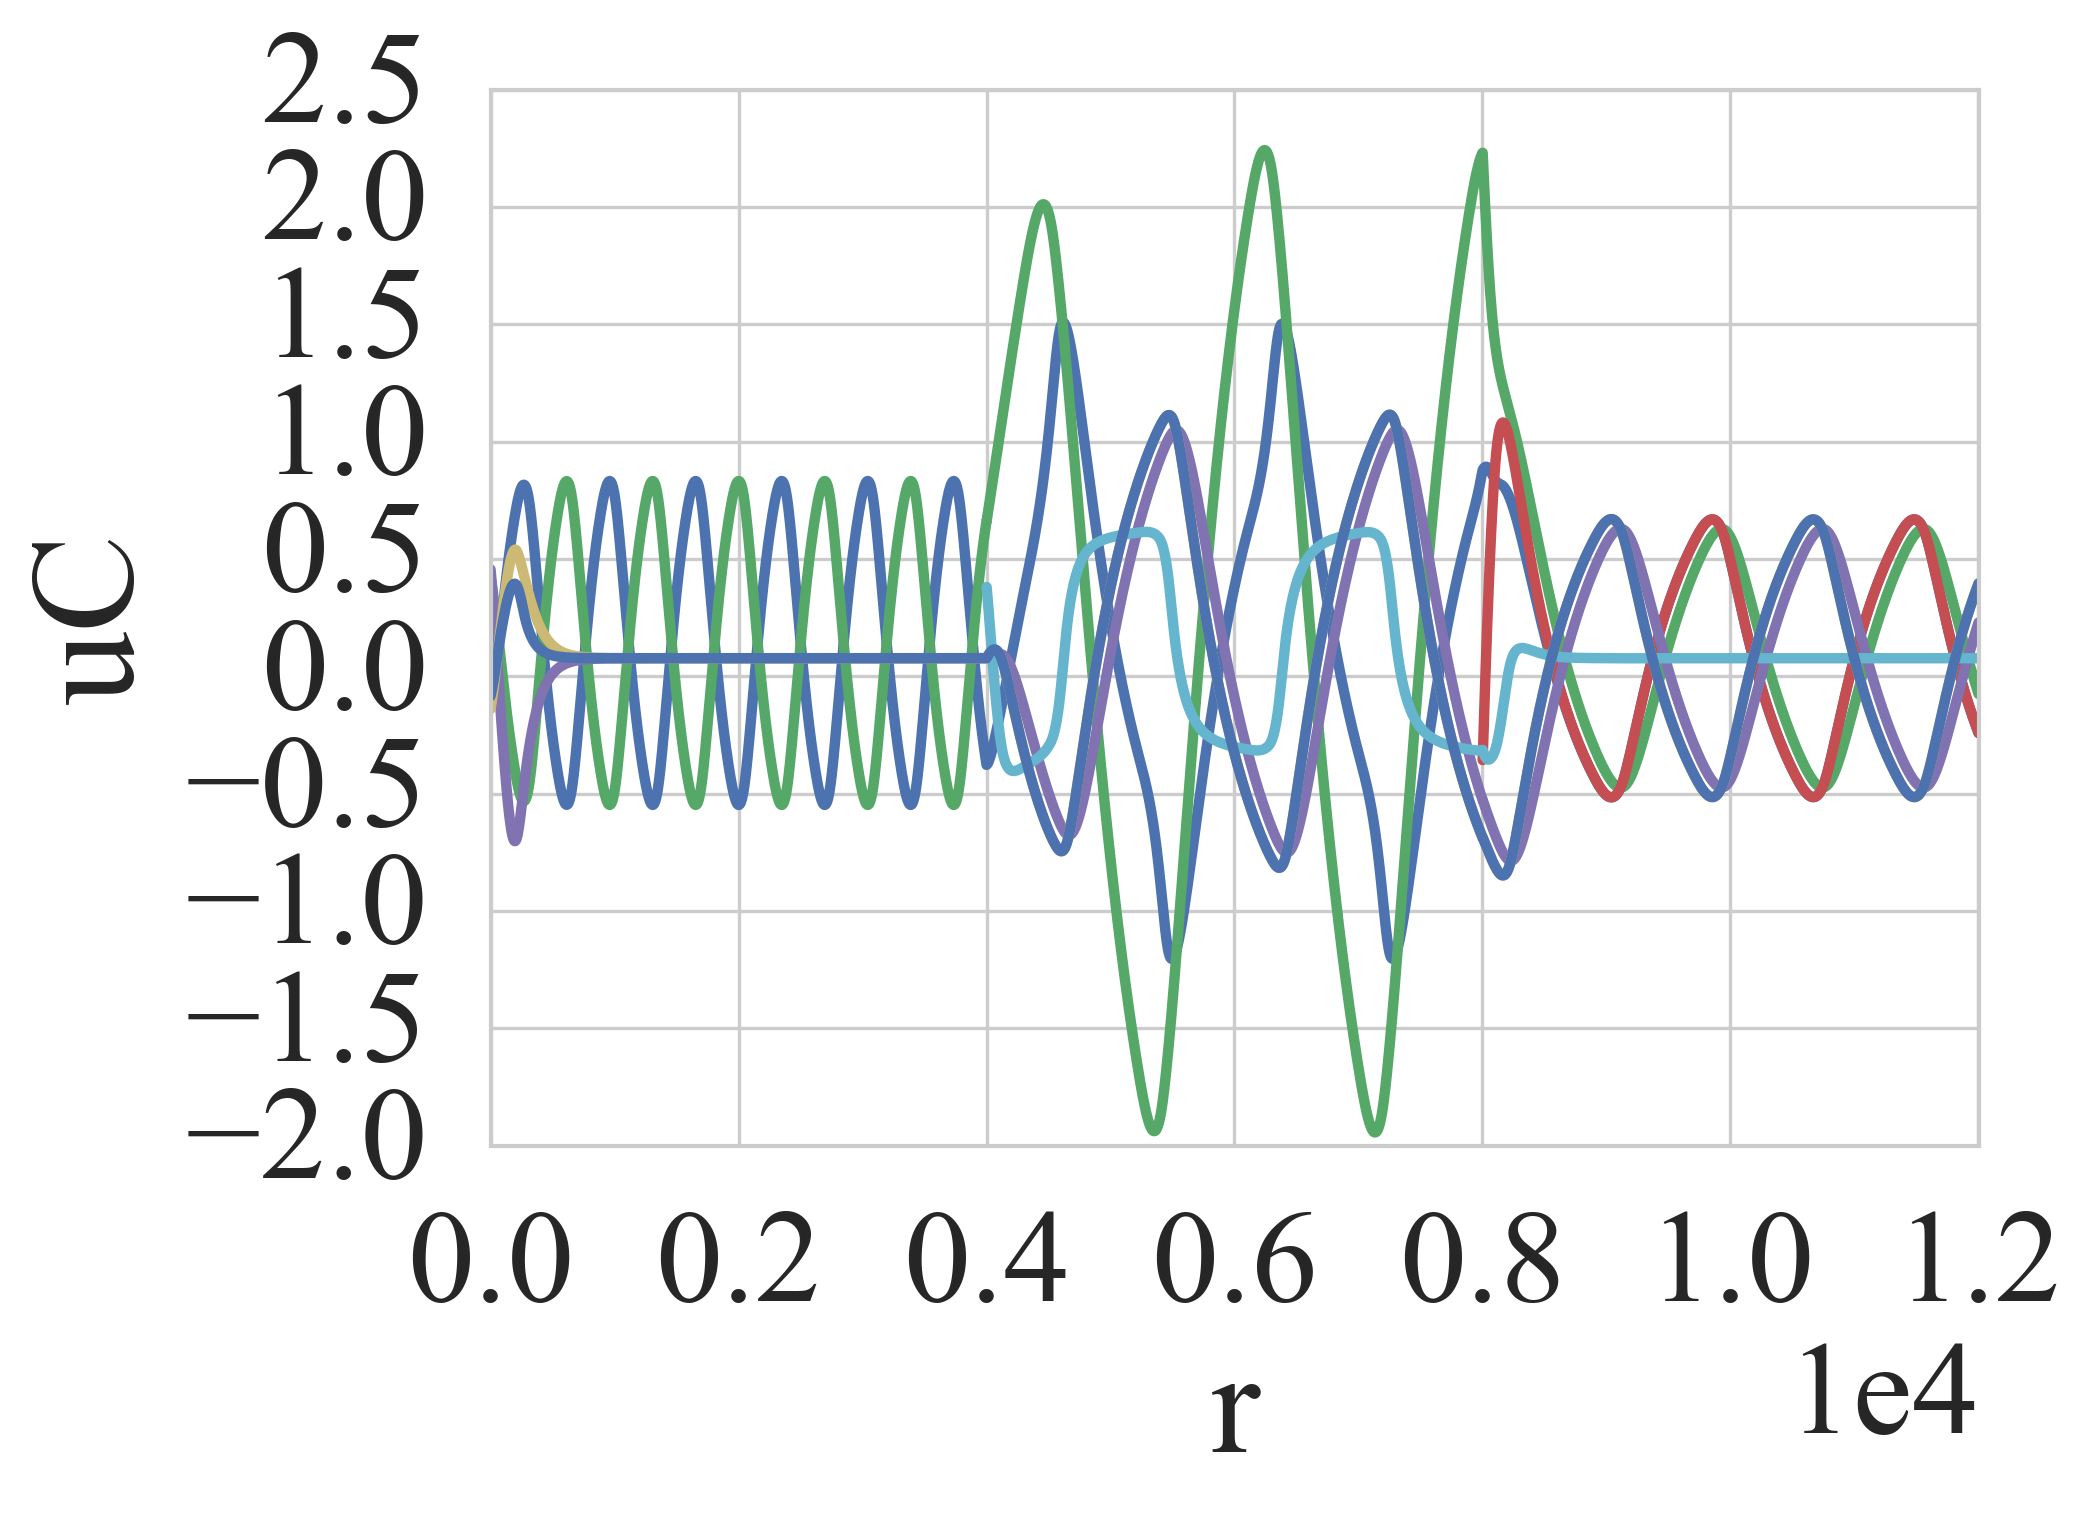
\includegraphics[width=0.4\linewidth,keepaspectratio]{./simulation/dumbbell/dumbbell_uC_changing_2.png}\label{fig:dumbbell_uC_changing_2}}
			
			\caption[Robustness of \Pns]{\Pns changing every $4000$ rounds.}
			\label{fig:robustness}
		\end{figure}

		These preliminary examples illustrate that changes in topology are naturally accommodated by the model. A more systematic investigation is a possible task for the future. Note, that when obtaining formal robustness properties for \Pns one may start by scanning related literature for classical electronic circuits.

	%!TEX root = ../../../../thesis.tex
\section{Discussion}

	We have proposed a preliminary model representing the oscillatory flows observed in networks formed by \P as currents in electrical networks. Our approach is based on the three-element Windkessel model. This approach has successfully been used in the past to model human cardiovascular networks which strongly resemble the vein networks of \P. The major difference between the two is the fact the slime mold does not have one strong central pump, \ie a heart, capable of producing flows. Rather each and every vein of the slime mold network may act as an independent peristaltic pump. Since a vein may be connected to several neighboring veins, non-trivial local interactions arise. To model emergent global oscillations we propose an extension to the Windkessel model, namely current controlled voltage sources. The resulting electronic \Pes are then connected according to a given topology to form a \Pn. The currents induced by such networks exhibit complex emergent flow patterns reminiscent of the flows observed in live \P.

	In a symbiotic fashion we combine analytic and numerical methods to explore the characteristics of the resulting model. We find first and foremost, that our model can be discretized and solved to yield current flows for \Pn of arbitrary topology. In practice we restrict our simulations to simple graph classes of limited size. They illustrate that the model is fully distributed as it requires no central control. It exhibits self-organization leading to coordinated flows and global anti-phase entrainment. In addition to that, we observe that the model is robust to changes of the underlying topology of \Pns. These are qualities attributed to live \P. Furthermore, we hope that our model also inherits some of the natural efficiency attributed to the behavior of \P. We are reduced to hope in this instance, because there is no way of asserting the statement in a systematic way.

	When we began thinking about meaningful extensions to the Windkessel model, we noticed that we were frequently faced with decisions about what assumptions to accept during the initial stages of modeling. First and foremost we decided to keep the model simple enough to be able to proof facts about it. This is in line with our desire to obtain a prospective candidate model that would serve as a basis for future attempts of natural computing. Thus we placed significant emphasis on implementing simplifying assumptions. Needless to say, these come at the cost of a reduced degree to which our model yields an accurate description of live \P. While this is unfortunate, in the context of computing inspired by nature it is of minor concern. In summary we decided to differentiate the original general model such, that modeling accuracy is sacrificed for ease of analytical treatment.

	Naturally, a different approach is necessary if your goal is synthesis of nature by means of computing. Here one seeks to obtain a model providing modeling accuracy and ultimately, predictive power. To do so, trading manageable complexity for a higher degree of modeling accuracy is acceptable. This entails replacing some of the following simplifying assumptions with more meaningful alternatives in order to obtain a model that is more interesting from a biophysical point of view. Perhaps most influential is the assumption that the electric resistance is constant and the same for all edges in the network. Note that the electrical resistance of \Pes translates to hydraulic resistance of veins in live \P, a quantity which strongly depends on the width of the veins. In fact, it is known that the distribution of widths in real \P is not constant but rather follows a gamma distribution. Clearly, the model could be made more meaningful by incorporating widths distributions of real \P graphs. Furthermore, the topologies of real \P graphs which are conveniently available could directly be used to run the model on. Yet another potential improvement is plainly apparent. In real \P there is evidence that changes in the vein diameter are directly coupled to the amount of flow passing through a vein. A simple rule suggested by Nakagaki et al. could easily be incorporated to make the model more physical.

	Incorporating these improvements including the move from simple small graphs to more complex \P graphs with more degrees of freedom for the edges likely shuts down all hopes of obtaining analytical statements about what is going on. Note that such a model may still be solvable given the right numerical tools. It could still form a valid basis for natural computing, however the analysis of obtained algorithms is expected to range somewhere between challenging and seemingly impossible. Naturally, analytic treatment and provable facts are of minor concern in this approach.

	Note that augmenting the Windkessel model such that modeling accuracy is maximized does not automatically yield a model with predictive power. What remains is to determine a way to set meaningful parameters of the \Pes. Unfortunately, the authors have no suggestion as to how to resolve this problem at present. A closer collaboration with biologist and biophysicists seems necessary to tackle this question.

	The authors are convinced that both described approaches supported by an augmented Windkessel model are valid and should be explored further. Indeed a manuscript is being prepared documenting our own attempts of deriving a distributed natural computing algorithm based on this model. While it is not necessary for a natural computing algorithm to closely resemble its source of inspiration, it would be nice if a connection between the way such an algorithm works and the way \P operates could be established. This task will likely require insights obtained in the pursuit of models of higher physical relevance and strengthen the interdisciplinary appeal of natural computing even further.


